\documentclass[12pt,a4paper,twoside]{report}
% Jeg forslår at man lige knytter en kommentar til de pakker man tilføjer så andre også kan benytte dem.

\usepackage[english]{babel} % Forklarer at dokumentet er engelsk
\usepackage{import}
\usepackage{verbatim} 
\usepackage[utf8]{inputenc} % Forklarer hvilket charset er dokumentet skrevet i
\usepackage[pdfborder={0 0 0 0}]{hyperref} % Indsætter url-adresser og ref-links korrekt. Disse kan vises som url adressen eller bare tekst og er klik-bare i pdf dokumentet. \href{URL}{text}
\usepackage{graphicx} % Bruges til at inkludere billede filer...
\usepackage{float} % Bruges blandt andet til H i figures
\bibliographystyle{plain} % Beskriver hvilken bibliografi stil der benyttes.
\usepackage[none]{hyphenat}
\usepackage{amsmath}
\usepackage{longtable}
\usepackage{listings}
\usepackage{rotating} %Bruges til at vende teksten vertikalt
\usepackage{framed} % Benyttes til at lave bokse om diverse ting.
\usepackage{multirow} % Benyttes til avancerede tabeller
\usepackage{pdfpages} % Bruges til indsættelse af pdf sider i LaTeX dokumentet.
\usepackage{fixme}
\usepackage{sidecap}


\newtheorem{def:recommend}{Definition} % Benyttes til definitioner i studierapporten

\title{The \textit{WAR} Programming Language}
\begin{document}
\pagestyle{empty}
\thispagestyle{empty}

\includepdf{forsidepdf.pdf}
\newpage\mbox{}\newpage
\thispagestyle{empty}
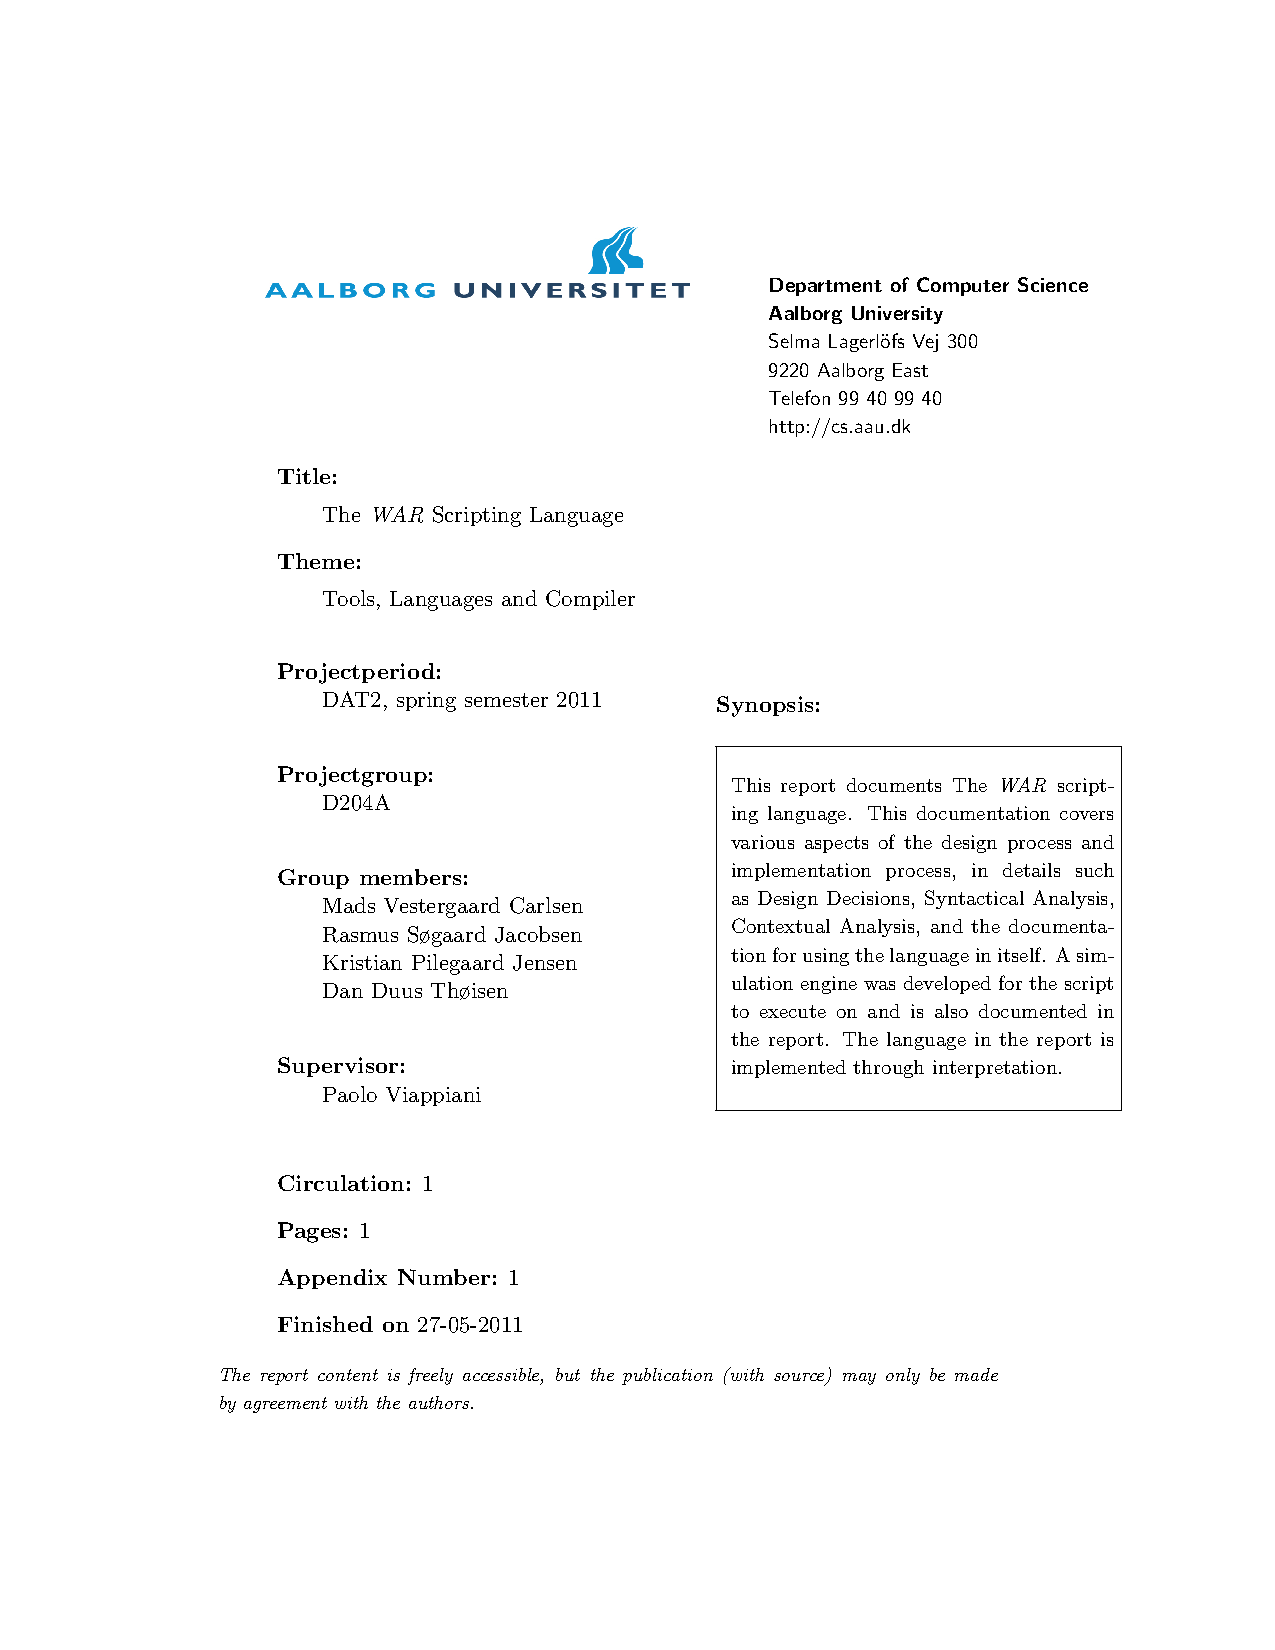
\includepdf{titelblad.pdf}
%1. Introduction - Why we chose the project, problem statement, overview of report structure


%This file only contains inputs!!!
\chapter{Game Description}
	\section{Syntax}
	The first step in writing our interpreter is to make a BNF of our language. BNF stands for {\it Backus Naur form} and is a way of
	structuring the language in a formal way, which will make it easy to implement. A BNF consists of a set of {\it production rules} and each
	production rule consists of: \\
	\begin{itemize}
		 \item Terminals: A {\it terminal } is a literal string that appears in the language in hand.
		 \item Non-terminal: A {\it non-terminal } consists of Non-terminals and Terminals, used for structuring the language.
	\end{itemize}
	
	\subsection*{Production Rule}
		A production rule has the form: \\
		$N ::= X$, \\
		where $X$ is a Non-terminal or a Terminal. \\
		
		The elements in a production rule can be identified by: \\
		Terminals are written in {\bf bold } and 
		Non-terminals are just written in plain text.
	\subsection*{Grouping of production rules}
		If we have two production rules on the form:\\
		$N ::= X$ \\
		$N ::= Y$ \\
		we are allowed to make a transformation: \\
		$N ::= X | Y$ \\
		Meaning $N$ is $X$ or $Y$ \\
	\subsection*{Example of a small BNF}
		\label{ex-bnf}
		\begin{center}
			\begin{tabular}{l l l}
				A		&	::=		&	 AB$ \mid $ B \\
				B		&	::=		&	{\bf b} $\mid$ {\bf n } $\mid$ {\bf f } \\
			\end{tabular}
		\end{center}
		This BNF would allow us to write programs like \\(We use $\rightarrow$ to show applying of a production rule): \\
		{\bf bnf}: A $\rightarrow$ AB $\rightarrow$ A{\bf f} $\rightarrow$ 
		AB{\bf f} $\rightarrow$A{\bf nf} $\rightarrow$ B{\bf nf}$\rightarrow${\bf bnf } \\
	
	\begin{comment}
	
	
	\subsubsection{Terminals}
	
	
		\begin{longtable}[l]{l}
			$\{$\\
			$\}$\\
			$>$\\
			$<$\\
			$($\\
			$)$\\
			$=$\\
			$+$\\
			$-$\\
			$*$\\
			$/$\\
			$\&$\\
			$|$\\
			$"$\\
			$,$\\
			$.$\\
			$;$\\
			$Attack$\\
			$AttackSpeed$\\
			$Behaviour$\\
			$Config$\\
			$Damage$\\
			$Distance$\\
			$else$\\
			$Grid$\\
			$Health$\
			$Height$\\
			$if$\\
			$Maxima$\\
			$Melee$\\
			$MoveAway$\\
			$Movement$\\
			$MoveTowards$\\
			$Position$\\
			$Range$\\
			$Ranged$\\
			$Regiment$\\
			$RegimentPosition$\\
			$Regiments$\\
			$Rules$\\
			$SearchForEnemies$\\
			$SearchForFriends$\\
			$Size$\\
			$Standards$\\
			$Team$\\
			$Teams$\\
			$Type$\\
			$While$\\
			$Width$\\
		\end{longtable}
%	\subsubsection{Nonterminals}
%		\begin{tabular}{l c}
%			Behaviour-Block   & Control-Structure   \\
%			Single-Command    & UnitStat 			\\
%			UnitStat-Name	  & Integer-Literal		\\
%			Comment			  & Team-File 			\\
%			Regiment-Block	  & Expression			\\
%			Operator		  & Config-File			\\
%			Grid-Block	      & Rules-Block 		\\
%			Maximums-Block	  & MaximumsStat		\\
%			MaximumsStat-Name & Standards-Block	 	\\
%			StandardsStat	  & StandardsStat-Name 	\\
%			Identifier		  & 					\\
%		\end{tabular}
\end{comment}
	\subsection{The BNF of the WAR Language}
		{\bf Notes}
		\begin{itemize}
			\item Digit represents one of the digits 0 through 9.
			\item Graphic represents a space or visible character.
			\item Letter represents one of the lower- or upper-case letters 'a','b',.....,or 'z'.
			\item eol represents an end-of-line 'character'.
		\end{itemize}
		\begin{center}
			\begin{longtable}{l l l}
				\endfirsthead
				\endhead
		Team-File					&	::=	&{\bf Team} Identifier Regiment-Block\\
		Identifier					&	::=	&Letter\\
									&$\mid$	&Identifier Digit\\
									&$\mid$	&Identifier Letter\\
		Block-Name					&	::=	&Identifier\\
		Regiment-Block				&	::=	&{\bf Regiment} Block-Name {\bf \{ } UnitStat Behaviour-Block \bf{\} }\\
									&$\mid$	&Regiment-Block {\bf Regiment} Block-Name\\
									&		&{\bf \{ } UnitStat Behaviour-Block \bf{\} }\\
		Behaviour-Block				&	::=	&{\bf Behaviour} Block-Name {\bf \{} Single-Command {\bf \}}  \\
									&$\mid$	& {\bf Behaviour} {\bf = } Block-Name{\bf ;} \\
		Regiment-Declaration			&	::=	&{\bf Regiment} Identifier {\bf =} Regiment-Search{\bf ;}\\
									&$\mid$	&{\bf Regiment} Identifier {\bf =} Block-Name{\bf ;}\\
		Regiment-Search				&	::=	&{\bf SearchForEnemies (}Parameters{\bf)}\\
									&$\mid$	&{\bf SearchForFriends(}Parameters{\bf)}\\
		RegimentStat				&	::=	&Identifier {\bf.} UnitStat-Type \\
		Parameters					&	::=	&UnitStat-Type Operator Integer-Literal\\
		 							&$\mid$	&Parameters{\bf ,} UnitStat-Type Operator Integer-Literal\\
		Single-Command				&	::=	&Control-Structure Single-Command \\
									&$\mid$	&Regiment-Declaration Single-Command\\
									&$\mid$	&UnitFunction Single-command\\
									&$\mid$	&Control-Structure\\
									&$\mid$	&UnitFunction\\
									&$\mid$	&Regiment-Declaration\\
		ElseIf-Structure			&	::=	&{\bf else if( } Expression{\bf )} {\bf \{ } Single-Command {\bf \} } ElseIf-Structure\\
									&$\mid$	&{\bf else if( } Expression{\bf )} {\bf \{ } Single-Command {\bf \} } \\
		Control-Structure			&	::=	&{\bf if( } Expression{\bf )} {\bf \{ } Single-Command {\bf \} }  \\
									&$\mid$	&{\bf if(} Expression {\bf )} {\bf \{ }Single-Command {\bf \}} \\
									&		&{\bf else } {\bf \{ }Single-Command {\bf \} } \\			
									&$\mid$	&{\bf if(} Expression {\bf )} {\bf \{ }Single-Command {\bf \}} \\
									&		&ElseIf-Structure {\bf else } {\bf \{ }Single-Command {\bf \} } \\
									&$\mid$	&{\bf if(} Expression {\bf )} {\bf \{ }Single-Command {\bf \}} ElseIf-Structure \\	
									&$\mid$	&{\bf while (} Expression {\bf )}{\bf \{ } Single-Command {\bf \}} \\
		Expression					&	::=	&Primary-Expression \\
									&$\mid$	&Expression Operator Primary-Expression \\
		Primary-Expression			&	::=	&(Expression)\\
									&$\mid$	&Integer-Literal \\
									&$\mid$	&UnitStat-Type \\
									&$\mid$	&RegimentStat \\
		Operator					&	::=	&$\boldsymbol {+}$\\
									&$\mid$	&$\boldsymbol {-}$\\
									&$\mid$	&$\boldsymbol {*}$\\
									&$\mid$	&$\boldsymbol {/}$\\
									&$\mid$	&$\boldsymbol {<}$\\
									&$\mid$	&$\boldsymbol {>}$\\
									&$\mid$	&$\boldsymbol {<=}$\\
									&$\mid$	&$\boldsymbol {>=}$\\
									&$\mid$	&$\boldsymbol {==}$\\
									&$\mid$	&$\boldsymbol {\&\&}$\\
									&$\mid$	&$\boldsymbol {\|}$\\
		UnitFunction				&	::=	&{\bf Attack(} Identifier {\bf );} \\
									&$\mid$	&{\bf MoveTowards(}Identifier {\bf );} \\
									&$\mid$	&{\bf MoveAway(} Identifier {\bf );} \\
		UnitStat					&	::=	&UnitStat-Declaration UnitStat \\
									&$\mid$	&UnitStat-Declaration \\
		UnitStat-Declaration		&	::=	&{\bf Size =} Integer-Literal{\bf ;} \\
									&$\mid$	&{\bf Type} = AttackType{\bf ;}\\
									&$\mid$	&{\bf  Range =} Integer-Literal{\bf;}\\
									&$\mid$	&{\bf Damage =} Integer-Literal{\bf ;}\\
									&$\mid$	&{\bf Movement = }Integer-Literal{\bf ;} \\				  
									&$\mid$	& {\bf RegimentPosition = Position(} Integer-Literal {\bf ,}\\
									&		& Integer-Literal {\bf );}\\
		UnitStat-Type				&	::=	&{\bf Size}\\
									&$\mid$	&{\bf Type}\\
									&$\mid$	&{\bf Range}\\
									&$\mid$	&{\bf Damage}\\
									&$\mid$	&{\bf Movement}\\
									&$\mid$	&{\bf AttackSpeed}\\
									&$\mid$	&{\bf Health}\\
									&$\mid$	&{\bf Distance}\\
		AttackType					&	::=	&{\bf Melee}\\
									&$\mid$	&{\bf Ranged}\\
		Integer-Literal				&	::=	&Digit\\
									&$\mid$	&Integer-Literal Digit\\
		Comment						&	::=	&{\bf //} Graphic-Literal eol\\
		Graphic-Literal				&	::=	&Graphic Graphic-Literal\\
									&$\mid$	&Graphic\\
		Config-File					&	::=	&{\bf Config} Grid-Block Rules-Block\\
		Grid-Block					&	::=	&{\bf Grid} Block-Name	 {\bf \{} GridStat \bf{\}}\\
		GridStat					&	::=	&GridStat-Declaration GridStat\\
									&$\mid$	&GridStat-Declaration \\
		GridStat-Declaration		&	::=	&{\bf Width = } Integer-Literal;\\
									&$\mid$	&{\bf Height = } Integer-Literal;\\
		Rules-Block					&	::=	&Standards-Block MaximumsBlock\\
		Maximums-Block				&	::=	&{\bf Maximums} {\bf \{} MaximumsStat {\bf \}} \\
		MaximumsStat				&	::=	&MaximumsStat-Declaration MaximumsStat\\
									&$\mid$	&MaximumsStat-Declaration\\
		MaximumsStat-Declaration	&	::=	&{\bf Regiments = } Integer-Literal{\bf ;}\\
									&$\mid$	&{\bf Teams = } Integer-Literal{\bf ;}\\
									&$\mid$	&{\bf Size = } Integer-Literal{\bf ;}\\
									&$\mid$	&{\bf Range = } Integer-Literal{\bf ;}\\
									&$\mid$	&{\bf Damage = } Integer-Literal{\bf ;}\\
									&$\mid$	&{\bf Movement = } Integer-Literal{\bf ;}\\
									&$\mid$	&{\bf AttackSpeed = } Integer-Literal{\bf ;}\\
									&$\mid$	&{\bf Health = } Integer-Literal{\bf ;}\\
		Standards-Block				&	::=	&{\bf Standards} {\bf \{ } UnitStat-Declaration Behaviour-Block\bf{\} }\\
			\end{longtable}
		\end{center}
		
		
	\subsection{EBNF}
		{\it EBNF} stands for {\it Extendend Backus Naur Form} and is, as the name refers to an extension of BNF.
		The EBNF allows us to use regular expressions to express production rules, which makes our rule set more compact and 
		easier to implement.
	
	\subsubsection*{Regular expressions}
		A regular expression is a convenient way of expressing strings. We use the following regular expressions: \\
		\begin{itemize}
			\item *(star): States that the terminal or non-terminal must be used 0 or more times.
			\item Parentheses: Used for grouping of non-terminals and terminals.
			\item $\epsilon$: Represents the empty string.
		\end{itemize}
		Please note that these regular expressions can only be used on the right side of the production rules. \\
		
		By using these regular expression we can \\
		transform the BNF example given in \ref{ex-bnf} to an EBNF: \\
		
		\begin{tabular}{l l l}
			B		&	::=		&	({\bf b} $\mid$ {\bf n } $\mid$ {\bf f })* \\
		\end{tabular}
		
		It's easy to see that the transformation made the rules more compact (we removed one the the production rules), but
		how do we transform a BNF to a EBNF in a systematic way? 
		This can be done by applying {\it left factorization }, {\it elimination of left recursion} and {\it substitution of non-terminals }.
		
		\subsubsection*{Left factorization}
			If we have a production rule on the form: \\
			\begin{tabular}{l l l}
				T		&	::=		&	AB$\mid$AC \\
			\end{tabular}
			
			We can do a left factorization: \\
			\begin{tabular}{l l l}
				T		&	::=		&	A(B$\mid$C) \\
			\end{tabular}
			
			This can be done because T will always start with an A and end with either a B or C.
			
		\subsubsection*{Elimination of left recursion}
			If we have a production rule on the form: \\
			\begin{tabular}{l l l}
				T		&	::=		&	A$\mid$TB \\
			\end{tabular}
			
			We can do an elimination of left recursion: \\
			\begin{tabular}{l l l}
				T		&	::=		&	A(B)* \\
			\end{tabular}
			
			To understand how we can do this look at the first production rule. To terminate the production rule we need 
			to put an A, so T will always consist of an A. When we are not selecting an A(, and terminating) we are only making B's, which is
			the same as B*.
		\subsubsection*{Substitution of non-terminals}
			If we have two production rules on the form: \\
			
			\begin{tabular}{l l l}
				T		&	::=		&	U $\mid$ AUC \\
				U		&	::=		&	{\bf ab} $\mid$ {\bf ba} \\
			\end{tabular} \\
			
			We can do a substitution of the non-terminal U for every production rule. This means that we 
			substitute any occurrence of U in a production rule with what is on the right hand side of U like this: \\
			
			\begin{tabular}{l l l}
				T		&	::=		&	({\bf ab} $\mid$ {\bf ba}) $\mid$ A ({\bf ab} $\mid$ {\bf ba})B \\
			\end{tabular}
	\subsection{The EBNF of the WAR Language}
		Left factorization, substituion of non-terminals 
		and elimination of left recursion was applied to transform the BNF to an EBNF. \\
		
		Substituion of non-terminals have removed the following non-terminals from the BNF: \\
		\begin{itemize}
			\item Else-If
			\item UnitStat
			\item Graphical-Literal
			\item GridStat
			\item MaximumsStat
		\end{itemize}
		
		\begin{center}
			\begin{longtable}{ l l l }
				\endfirsthead
				\endhead
		Team-File					&	::=	&{\bf Team} Identifier Regiment-Block*\\
		Identifier					&	::=	&Letter (Letter $\mid$ Digit)*\\
		Block-Name					&	::=	&Identifier\\
		Regiment-Block				&	::=	&{\bf Regiment} Block-Name {\bf \{ } \\
									&		&UnitStat-Declaration Behaviour-Block \bf{\} }\\
		Behaviour-Block				&	::=	&{\bf Behaviour}(Identifier{\bf \{ }Single-Command \bf{\} } $\mid$ {\bf $=$} Identifier)\\
		Regiment-Declaration		&	::=	&{\bf Regiment} Identifier {\bf =} Regiment-Search{\bf ;}\\
									&$\mid$	&{\bf Regiment} Identifier {\bf =} Block-Name{\bf ;}\\
		Regiment-Search				&	::=	&{\bf SearchForEnemies (} Parameters {\bf )}\\
									&$\mid$	&{\bf SearchForFriends(} Parameters {\bf )}\\
		RegimentStat				&	::=	&Identifier{\bf.}UnitStat-Type \\
		Parameters					&	::=	&UnitStat-Type Operator Integer-Literal\\
									&		&({\bf ,}UnitStat-Type Operator Integer-Literal)*\\
		Single-Command				&	::=	&(Control-Structure $\mid$ UnitFunction $\mid$ Regiment-Declaration)*\\
									&		&(Control-Structure $\mid$ UnitFunction $\mid$ Regiment-Declaration)\\		
		Control-Structure			&	::=	&if(Expression) \bf{\{}Single-Command \bf{\}}\\
									&		&(\bf{else if(}Expression\bf{)\{ }Single-Command\bf{ \}})* \\
									&		&($\epsilon$ $\mid$ else \bf{\{ }Single-Command \bf{\} }\\					   
									&$\mid$	&while(Expression)\bf{\{ } Single-Command \bf{\}}\\
		Expression					&	::=	&Primary-Expression (Operator Primary-Expression)*\\
		Primary-Expression			&	::=	&(Expression)\\
									&$\mid$	&Integer-Literal \\
									&$\mid$	&UnitStat-Type\\
									&$\mid$	&RegimentStat \\	
		Operator					&	::=	&$\boldsymbol {+}$\\
									&$\mid$	&$\boldsymbol {-}$\\
									&$\mid$	&$\boldsymbol {*}$\\
									&$\mid$	&$\boldsymbol {/}$\\
									&$\mid$	&$\boldsymbol {<}$\\
									&$\mid$	&$\boldsymbol {>}$\\
									&$\mid$	&$\boldsymbol {<=}$\\
									&$\mid$	&$\boldsymbol {>=}$\\
									&$\mid$	&$\boldsymbol {==}$\\
									&$\mid$	&$\boldsymbol {\&\&}$\\
									&$\mid$	&$\boldsymbol {\|}$\\
		UnitFunction				&	::=	&({\bf Attack} $\mid$ {\bf MoveTowards} $\mid${\bf MoveAway}){\bf (} Identifier {\bf );}\\
		UnitStat-Declaration		&	::=	&({\bf Size}$\mid${\bf Range}$\mid${\bf Damage} $\mid${\bf Movement}\\ 
									&		&$\mid$ {\bf AttackSpeed}$\mid${\bf Health}) ${\bf = }$ Integer-Literal{\bf ;} \\
									&$\mid$	&{\bf RegimentPosition =} \\
									&		&{\bf Position(}Integer-Literal{\bf ,}Integer-Literal{\bf );}\\
									&$\mid$	&{\bf Type} = AttackType{\bf ;}\\
		UnitStat-Type				&	::=	&({\bf Size}$\mid${\bf Range}$\mid${\bf Damage} $\mid$\\
									&		&{\bf Movement}$\mid$ {\bf AttackSpeed}$\mid${\bf Health}$\mid${\bf Distance})\\ 
		AttackType					&	::=	&{\bf Melee} $\mid$ {\bf Ranged} \\
		Integer-Literal				&	::=	&Digit Digit*\\
		Comment						&	::=	&{\bf //} Graphic* eol\\
		Config-File					&	::=	&{\bf Config} Grid-Block Rules-Block  		\\
		Grid-Block					&	::=	&{\bf Grid} Block-Name	 {\bf \{} GridStat-Declaration* \bf{\}} \\
		GridStat-Declaration		&	::=	&({\bf Width} $\mid$ {\bf Height})=  Integer-Literal{\bf ;} \\	
		Rules-Block					&	::=	&Standards-Block MaximumsBlock 				\\
		Maximums-Block				&	::=	&{\bf Maximums} {\bf \{} (MaximumsStat-Declaration)* {\bf \}}\\
		MaximumsStat-Declaration	&	::=	&({\bf Regiments }$\mid${\bf Teams}$\mid${\bf Size}$\mid$\\
									&		&{\bf Range}$\mid${\bf Damage}$\mid${\bf Movement}$\mid$\\
									&		&{\bf AttackSpeed}$\mid${\bf Health}) =  Integer-Literal{\bf ;}\\
		Standards-Block				&	::=	&{\bf Standards} {\bf \{ } UnitStat-Declaration* Behaviour-Block\bf{\} }		\\
			\end{longtable}
		\end{center}					     

	\section{Construction of the parser}
	In this section we will describe how one can construct a parser from a EBNF, but first we will describe how a parser is and how it works.
	
	\subsection{Parsing}
		The job of a parser is to check if a program is correct and 
		to determine the structure of the program, usually done by constructing tree structure.
		There are two ways of checking this {\it Bottom-up Parsing} and {\it Top-Down Parsing}.
		
		\subsubsection*{Bottom-up Parsing}
			This way of parsing takes simple structures and combining them to more complex structures.
			We show how this type of parsing works by applying Bottom-up parsing on this code written in : \\
			{\bf Maximums \{ Regiments = 5;\} }
			
			\begin{enumerate}
				\item Looks at 5 - Identifies it as an Integer-literal
				\item Looks at 5* -
			\end{enumerate}
			
	\section{Semantics}
\label{sec:conanal}
This section will define the scope and type rules of WAR.
	\subsection{Scope rules}
		A scope is a block of code, in WAR one is able to denote a new scope by using $\{$ to start the scope and $\}$.
		A scope placed inside another scope is called a {\it nested scope}. A {\it scope level} denotes how nested a given scope is,
		e.g. identifiers at scope level 0 is outside any scope, identifiers at scope level 1 is inside one scope etc.
		\begin{lstlisting}
		Scope
		{
			//Scope level 1
			identifier = 2
			Scope
			{
				//Scope level 2
				identifier = 2
			}
		}
		\end{lstlisting}
		
		Scope rules dictate the accessibility of identifiers from one scope to another.
	
	%These are the rules that defines how the identifiers must be read, and where to declare them - also known as identification.
	The WAR language has a nested block-structure which means we may have constants or variables can be defined in multiple scope levels. 
	Scope rules may be defined in levels, such that a declaration in the outermost block is at scope level 1, however, since the language has no declaration of variables, only constants, it works the same way. If you declare the $Size$ of a regiment at scope level 1, you can use $Size$ in all the higher scope levels. Declarations inside a block are referred to as being local in that block.

	The use of a nested block structure we follow some basic scope rules:
	\begin{wrapfigure}{r}{0.5\textwidth}
		\begin{center}
			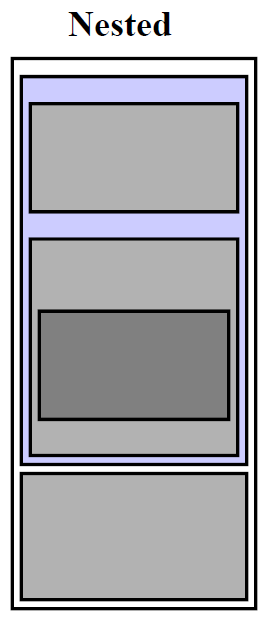
\includegraphics[scale=0.5]{rapport/5/figures/nested_block_structure}
		\end{center}	
		\caption{Illustration of the nested block structure}
		\label{nested_block_structure}
	\end{wrapfigure}


	%INCLUDE BIBLIOGRAPHY!!!	
	\begin{itemize}
	\item No identifier may be declared more than once within the same block (at the same level) %SPO
	\item For any applied occurrence there must be a corresponding occurrence, either within the same block or block which is higher up in the nesting. %SPO
	%INCLUDE BIBL...
	\end{itemize}
	
	
	Referring to figure \ref{nested_block_structure} which demonstrates the functioning of a nested block structure visually. Initially we consider how the nested block structure works in general and later an example of how the nested block structure works in the WAR programming language.
	
	One can have as many and as few blocks as needed, and every sub-block of an existing block, can use all the variables that have been declared in blocks over itself. 
	
	
	%Her kommer noget kode af vores egen for at beskrive hvordan nested block structure virker hos os.
		
\newpage
	
	
%Page 142 i Brown!! :D
		
\subsection{Type rules}
	These are the rules that checks the expressions form, and the type validity.
	
	\subsubsection*{Type rule of $<$}
		$E1 < E2$ is type correct and of type Boolean
		if $E1$ and $E2$ are type correct and of type Integer
	\subsubsection*{Type rule of $>$}
		$E1 > E2$ is type correct and of type Boolean
		if $E1$ and $E2$ are type correct and of type Integer
	\subsubsection*{Type rule of $==$}
		$E1 == E2$ is type correct and of type Boolean
		if $E1$ and $E2$ are type correct and of type Integer
	\subsubsection*{Type rule of $>=$}
		$E1 >= E2$ is type correct and of type Boolean
		if $E1$ and $E2$ are type correct and of type Integer
	\subsubsection*{Type rule of $<=$}
		$E1 <= E2$ is type correct and of type Boolean
		if $E1$ and $E2$ are type correct and of type Integer
	\subsubsection*{Type rule of $while$}
		$while(E){C}$ is type correct
		if $E$ is of type Boolean and $C$ is type correct
	\subsubsection*{Type rule of $if$}
		$if(E){C}$ is type correct
		if $E$ is of type Boolean and $C$ is type correct
	\subsubsection*{Type rule of $else if$}
		$else if(E){C}$ is type correct
		if $E$ is of type Boolean and $C$ is type correct
	\subsubsection*{Type rule of $else$}
		$else{C}$ is type correct
		if $C$ is type correct
	
	\subsubsection*{Type rule of $Position$}
		$Position(I1,I2)$ is type correct and of type Position
		if $I1$ and $I2$ are type correct and of type Integer	
	


%2. Game Description

%This file only contains inputs!!!
\chapter{Game Description}
	\section{Syntax}
	The first step in writing our interpreter is to make a BNF of our language. BNF stands for {\it Backus Naur form} and is a way of
	structuring the language in a formal way, which will make it easy to implement. A BNF consists of a set of {\it production rules} and each
	production rule consists of: \\
	\begin{itemize}
		 \item Terminals: A {\it terminal } is a literal string that appears in the language in hand.
		 \item Non-terminal: A {\it non-terminal } consists of Non-terminals and Terminals, used for structuring the language.
	\end{itemize}
	
	\subsection*{Production Rule}
		A production rule has the form: \\
		$N ::= X$, \\
		where $X$ is a Non-terminal or a Terminal. \\
		
		The elements in a production rule can be identified by: \\
		Terminals are written in {\bf bold } and 
		Non-terminals are just written in plain text.
	\subsection*{Grouping of production rules}
		If we have two production rules on the form:\\
		$N ::= X$ \\
		$N ::= Y$ \\
		we are allowed to make a transformation: \\
		$N ::= X | Y$ \\
		Meaning $N$ is $X$ or $Y$ \\
	\subsection*{Example of a small BNF}
		\label{ex-bnf}
		\begin{center}
			\begin{tabular}{l l l}
				A		&	::=		&	 AB$ \mid $ B \\
				B		&	::=		&	{\bf b} $\mid$ {\bf n } $\mid$ {\bf f } \\
			\end{tabular}
		\end{center}
		This BNF would allow us to write programs like \\(We use $\rightarrow$ to show applying of a production rule): \\
		{\bf bnf}: A $\rightarrow$ AB $\rightarrow$ A{\bf f} $\rightarrow$ 
		AB{\bf f} $\rightarrow$A{\bf nf} $\rightarrow$ B{\bf nf}$\rightarrow${\bf bnf } \\
	
	\begin{comment}
	
	
	\subsubsection{Terminals}
	
	
		\begin{longtable}[l]{l}
			$\{$\\
			$\}$\\
			$>$\\
			$<$\\
			$($\\
			$)$\\
			$=$\\
			$+$\\
			$-$\\
			$*$\\
			$/$\\
			$\&$\\
			$|$\\
			$"$\\
			$,$\\
			$.$\\
			$;$\\
			$Attack$\\
			$AttackSpeed$\\
			$Behaviour$\\
			$Config$\\
			$Damage$\\
			$Distance$\\
			$else$\\
			$Grid$\\
			$Health$\
			$Height$\\
			$if$\\
			$Maxima$\\
			$Melee$\\
			$MoveAway$\\
			$Movement$\\
			$MoveTowards$\\
			$Position$\\
			$Range$\\
			$Ranged$\\
			$Regiment$\\
			$RegimentPosition$\\
			$Regiments$\\
			$Rules$\\
			$SearchForEnemies$\\
			$SearchForFriends$\\
			$Size$\\
			$Standards$\\
			$Team$\\
			$Teams$\\
			$Type$\\
			$While$\\
			$Width$\\
		\end{longtable}
%	\subsubsection{Nonterminals}
%		\begin{tabular}{l c}
%			Behaviour-Block   & Control-Structure   \\
%			Single-Command    & UnitStat 			\\
%			UnitStat-Name	  & Integer-Literal		\\
%			Comment			  & Team-File 			\\
%			Regiment-Block	  & Expression			\\
%			Operator		  & Config-File			\\
%			Grid-Block	      & Rules-Block 		\\
%			Maximums-Block	  & MaximumsStat		\\
%			MaximumsStat-Name & Standards-Block	 	\\
%			StandardsStat	  & StandardsStat-Name 	\\
%			Identifier		  & 					\\
%		\end{tabular}
\end{comment}
	\subsection{The BNF of the WAR Language}
		{\bf Notes}
		\begin{itemize}
			\item Digit represents one of the digits 0 through 9.
			\item Graphic represents a space or visible character.
			\item Letter represents one of the lower- or upper-case letters 'a','b',.....,or 'z'.
			\item eol represents an end-of-line 'character'.
		\end{itemize}
		\begin{center}
			\begin{longtable}{l l l}
				\endfirsthead
				\endhead
		Team-File					&	::=	&{\bf Team} Identifier Regiment-Block\\
		Identifier					&	::=	&Letter\\
									&$\mid$	&Identifier Digit\\
									&$\mid$	&Identifier Letter\\
		Block-Name					&	::=	&Identifier\\
		Regiment-Block				&	::=	&{\bf Regiment} Block-Name {\bf \{ } UnitStat Behaviour-Block \bf{\} }\\
									&$\mid$	&Regiment-Block {\bf Regiment} Block-Name\\
									&		&{\bf \{ } UnitStat Behaviour-Block \bf{\} }\\
		Behaviour-Block				&	::=	&{\bf Behaviour} Block-Name {\bf \{} Single-Command {\bf \}}  \\
									&$\mid$	& {\bf Behaviour} {\bf = } Block-Name{\bf ;} \\
		Regiment-Declaration			&	::=	&{\bf Regiment} Identifier {\bf =} Regiment-Search{\bf ;}\\
									&$\mid$	&{\bf Regiment} Identifier {\bf =} Block-Name{\bf ;}\\
		Regiment-Search				&	::=	&{\bf SearchForEnemies (}Parameters{\bf)}\\
									&$\mid$	&{\bf SearchForFriends(}Parameters{\bf)}\\
		RegimentStat				&	::=	&Identifier {\bf.} UnitStat-Type \\
		Parameters					&	::=	&UnitStat-Type Operator Integer-Literal\\
		 							&$\mid$	&Parameters{\bf ,} UnitStat-Type Operator Integer-Literal\\
		Single-Command				&	::=	&Control-Structure Single-Command \\
									&$\mid$	&Regiment-Declaration Single-Command\\
									&$\mid$	&UnitFunction Single-command\\
									&$\mid$	&Control-Structure\\
									&$\mid$	&UnitFunction\\
									&$\mid$	&Regiment-Declaration\\
		ElseIf-Structure			&	::=	&{\bf else if( } Expression{\bf )} {\bf \{ } Single-Command {\bf \} } ElseIf-Structure\\
									&$\mid$	&{\bf else if( } Expression{\bf )} {\bf \{ } Single-Command {\bf \} } \\
		Control-Structure			&	::=	&{\bf if( } Expression{\bf )} {\bf \{ } Single-Command {\bf \} }  \\
									&$\mid$	&{\bf if(} Expression {\bf )} {\bf \{ }Single-Command {\bf \}} \\
									&		&{\bf else } {\bf \{ }Single-Command {\bf \} } \\			
									&$\mid$	&{\bf if(} Expression {\bf )} {\bf \{ }Single-Command {\bf \}} \\
									&		&ElseIf-Structure {\bf else } {\bf \{ }Single-Command {\bf \} } \\
									&$\mid$	&{\bf if(} Expression {\bf )} {\bf \{ }Single-Command {\bf \}} ElseIf-Structure \\	
									&$\mid$	&{\bf while (} Expression {\bf )}{\bf \{ } Single-Command {\bf \}} \\
		Expression					&	::=	&Primary-Expression \\
									&$\mid$	&Expression Operator Primary-Expression \\
		Primary-Expression			&	::=	&(Expression)\\
									&$\mid$	&Integer-Literal \\
									&$\mid$	&UnitStat-Type \\
									&$\mid$	&RegimentStat \\
		Operator					&	::=	&$\boldsymbol {+}$\\
									&$\mid$	&$\boldsymbol {-}$\\
									&$\mid$	&$\boldsymbol {*}$\\
									&$\mid$	&$\boldsymbol {/}$\\
									&$\mid$	&$\boldsymbol {<}$\\
									&$\mid$	&$\boldsymbol {>}$\\
									&$\mid$	&$\boldsymbol {<=}$\\
									&$\mid$	&$\boldsymbol {>=}$\\
									&$\mid$	&$\boldsymbol {==}$\\
									&$\mid$	&$\boldsymbol {\&\&}$\\
									&$\mid$	&$\boldsymbol {\|}$\\
		UnitFunction				&	::=	&{\bf Attack(} Identifier {\bf );} \\
									&$\mid$	&{\bf MoveTowards(}Identifier {\bf );} \\
									&$\mid$	&{\bf MoveAway(} Identifier {\bf );} \\
		UnitStat					&	::=	&UnitStat-Declaration UnitStat \\
									&$\mid$	&UnitStat-Declaration \\
		UnitStat-Declaration		&	::=	&{\bf Size =} Integer-Literal{\bf ;} \\
									&$\mid$	&{\bf Type} = AttackType{\bf ;}\\
									&$\mid$	&{\bf  Range =} Integer-Literal{\bf;}\\
									&$\mid$	&{\bf Damage =} Integer-Literal{\bf ;}\\
									&$\mid$	&{\bf Movement = }Integer-Literal{\bf ;} \\				  
									&$\mid$	& {\bf RegimentPosition = Position(} Integer-Literal {\bf ,}\\
									&		& Integer-Literal {\bf );}\\
		UnitStat-Type				&	::=	&{\bf Size}\\
									&$\mid$	&{\bf Type}\\
									&$\mid$	&{\bf Range}\\
									&$\mid$	&{\bf Damage}\\
									&$\mid$	&{\bf Movement}\\
									&$\mid$	&{\bf AttackSpeed}\\
									&$\mid$	&{\bf Health}\\
									&$\mid$	&{\bf Distance}\\
		AttackType					&	::=	&{\bf Melee}\\
									&$\mid$	&{\bf Ranged}\\
		Integer-Literal				&	::=	&Digit\\
									&$\mid$	&Integer-Literal Digit\\
		Comment						&	::=	&{\bf //} Graphic-Literal eol\\
		Graphic-Literal				&	::=	&Graphic Graphic-Literal\\
									&$\mid$	&Graphic\\
		Config-File					&	::=	&{\bf Config} Grid-Block Rules-Block\\
		Grid-Block					&	::=	&{\bf Grid} Block-Name	 {\bf \{} GridStat \bf{\}}\\
		GridStat					&	::=	&GridStat-Declaration GridStat\\
									&$\mid$	&GridStat-Declaration \\
		GridStat-Declaration		&	::=	&{\bf Width = } Integer-Literal;\\
									&$\mid$	&{\bf Height = } Integer-Literal;\\
		Rules-Block					&	::=	&Standards-Block MaximumsBlock\\
		Maximums-Block				&	::=	&{\bf Maximums} {\bf \{} MaximumsStat {\bf \}} \\
		MaximumsStat				&	::=	&MaximumsStat-Declaration MaximumsStat\\
									&$\mid$	&MaximumsStat-Declaration\\
		MaximumsStat-Declaration	&	::=	&{\bf Regiments = } Integer-Literal{\bf ;}\\
									&$\mid$	&{\bf Teams = } Integer-Literal{\bf ;}\\
									&$\mid$	&{\bf Size = } Integer-Literal{\bf ;}\\
									&$\mid$	&{\bf Range = } Integer-Literal{\bf ;}\\
									&$\mid$	&{\bf Damage = } Integer-Literal{\bf ;}\\
									&$\mid$	&{\bf Movement = } Integer-Literal{\bf ;}\\
									&$\mid$	&{\bf AttackSpeed = } Integer-Literal{\bf ;}\\
									&$\mid$	&{\bf Health = } Integer-Literal{\bf ;}\\
		Standards-Block				&	::=	&{\bf Standards} {\bf \{ } UnitStat-Declaration Behaviour-Block\bf{\} }\\
			\end{longtable}
		\end{center}
		
		
	\subsection{EBNF}
		{\it EBNF} stands for {\it Extendend Backus Naur Form} and is, as the name refers to an extension of BNF.
		The EBNF allows us to use regular expressions to express production rules, which makes our rule set more compact and 
		easier to implement.
	
	\subsubsection*{Regular expressions}
		A regular expression is a convenient way of expressing strings. We use the following regular expressions: \\
		\begin{itemize}
			\item *(star): States that the terminal or non-terminal must be used 0 or more times.
			\item Parentheses: Used for grouping of non-terminals and terminals.
			\item $\epsilon$: Represents the empty string.
		\end{itemize}
		Please note that these regular expressions can only be used on the right side of the production rules. \\
		
		By using these regular expression we can \\
		transform the BNF example given in \ref{ex-bnf} to an EBNF: \\
		
		\begin{tabular}{l l l}
			B		&	::=		&	({\bf b} $\mid$ {\bf n } $\mid$ {\bf f })* \\
		\end{tabular}
		
		It's easy to see that the transformation made the rules more compact (we removed one the the production rules), but
		how do we transform a BNF to a EBNF in a systematic way? 
		This can be done by applying {\it left factorization }, {\it elimination of left recursion} and {\it substitution of non-terminals }.
		
		\subsubsection*{Left factorization}
			If we have a production rule on the form: \\
			\begin{tabular}{l l l}
				T		&	::=		&	AB$\mid$AC \\
			\end{tabular}
			
			We can do a left factorization: \\
			\begin{tabular}{l l l}
				T		&	::=		&	A(B$\mid$C) \\
			\end{tabular}
			
			This can be done because T will always start with an A and end with either a B or C.
			
		\subsubsection*{Elimination of left recursion}
			If we have a production rule on the form: \\
			\begin{tabular}{l l l}
				T		&	::=		&	A$\mid$TB \\
			\end{tabular}
			
			We can do an elimination of left recursion: \\
			\begin{tabular}{l l l}
				T		&	::=		&	A(B)* \\
			\end{tabular}
			
			To understand how we can do this look at the first production rule. To terminate the production rule we need 
			to put an A, so T will always consist of an A. When we are not selecting an A(, and terminating) we are only making B's, which is
			the same as B*.
		\subsubsection*{Substitution of non-terminals}
			If we have two production rules on the form: \\
			
			\begin{tabular}{l l l}
				T		&	::=		&	U $\mid$ AUC \\
				U		&	::=		&	{\bf ab} $\mid$ {\bf ba} \\
			\end{tabular} \\
			
			We can do a substitution of the non-terminal U for every production rule. This means that we 
			substitute any occurrence of U in a production rule with what is on the right hand side of U like this: \\
			
			\begin{tabular}{l l l}
				T		&	::=		&	({\bf ab} $\mid$ {\bf ba}) $\mid$ A ({\bf ab} $\mid$ {\bf ba})B \\
			\end{tabular}
	\subsection{The EBNF of the WAR Language}
		Left factorization, substituion of non-terminals 
		and elimination of left recursion was applied to transform the BNF to an EBNF. \\
		
		Substituion of non-terminals have removed the following non-terminals from the BNF: \\
		\begin{itemize}
			\item Else-If
			\item UnitStat
			\item Graphical-Literal
			\item GridStat
			\item MaximumsStat
		\end{itemize}
		
		\begin{center}
			\begin{longtable}{ l l l }
				\endfirsthead
				\endhead
		Team-File					&	::=	&{\bf Team} Identifier Regiment-Block*\\
		Identifier					&	::=	&Letter (Letter $\mid$ Digit)*\\
		Block-Name					&	::=	&Identifier\\
		Regiment-Block				&	::=	&{\bf Regiment} Block-Name {\bf \{ } \\
									&		&UnitStat-Declaration Behaviour-Block \bf{\} }\\
		Behaviour-Block				&	::=	&{\bf Behaviour}(Identifier{\bf \{ }Single-Command \bf{\} } $\mid$ {\bf $=$} Identifier)\\
		Regiment-Declaration		&	::=	&{\bf Regiment} Identifier {\bf =} Regiment-Search{\bf ;}\\
									&$\mid$	&{\bf Regiment} Identifier {\bf =} Block-Name{\bf ;}\\
		Regiment-Search				&	::=	&{\bf SearchForEnemies (} Parameters {\bf )}\\
									&$\mid$	&{\bf SearchForFriends(} Parameters {\bf )}\\
		RegimentStat				&	::=	&Identifier{\bf.}UnitStat-Type \\
		Parameters					&	::=	&UnitStat-Type Operator Integer-Literal\\
									&		&({\bf ,}UnitStat-Type Operator Integer-Literal)*\\
		Single-Command				&	::=	&(Control-Structure $\mid$ UnitFunction $\mid$ Regiment-Declaration)*\\
									&		&(Control-Structure $\mid$ UnitFunction $\mid$ Regiment-Declaration)\\		
		Control-Structure			&	::=	&if(Expression) \bf{\{}Single-Command \bf{\}}\\
									&		&(\bf{else if(}Expression\bf{)\{ }Single-Command\bf{ \}})* \\
									&		&($\epsilon$ $\mid$ else \bf{\{ }Single-Command \bf{\} }\\					   
									&$\mid$	&while(Expression)\bf{\{ } Single-Command \bf{\}}\\
		Expression					&	::=	&Primary-Expression (Operator Primary-Expression)*\\
		Primary-Expression			&	::=	&(Expression)\\
									&$\mid$	&Integer-Literal \\
									&$\mid$	&UnitStat-Type\\
									&$\mid$	&RegimentStat \\	
		Operator					&	::=	&$\boldsymbol {+}$\\
									&$\mid$	&$\boldsymbol {-}$\\
									&$\mid$	&$\boldsymbol {*}$\\
									&$\mid$	&$\boldsymbol {/}$\\
									&$\mid$	&$\boldsymbol {<}$\\
									&$\mid$	&$\boldsymbol {>}$\\
									&$\mid$	&$\boldsymbol {<=}$\\
									&$\mid$	&$\boldsymbol {>=}$\\
									&$\mid$	&$\boldsymbol {==}$\\
									&$\mid$	&$\boldsymbol {\&\&}$\\
									&$\mid$	&$\boldsymbol {\|}$\\
		UnitFunction				&	::=	&({\bf Attack} $\mid$ {\bf MoveTowards} $\mid${\bf MoveAway}){\bf (} Identifier {\bf );}\\
		UnitStat-Declaration		&	::=	&({\bf Size}$\mid${\bf Range}$\mid${\bf Damage} $\mid${\bf Movement}\\ 
									&		&$\mid$ {\bf AttackSpeed}$\mid${\bf Health}) ${\bf = }$ Integer-Literal{\bf ;} \\
									&$\mid$	&{\bf RegimentPosition =} \\
									&		&{\bf Position(}Integer-Literal{\bf ,}Integer-Literal{\bf );}\\
									&$\mid$	&{\bf Type} = AttackType{\bf ;}\\
		UnitStat-Type				&	::=	&({\bf Size}$\mid${\bf Range}$\mid${\bf Damage} $\mid$\\
									&		&{\bf Movement}$\mid$ {\bf AttackSpeed}$\mid${\bf Health}$\mid${\bf Distance})\\ 
		AttackType					&	::=	&{\bf Melee} $\mid$ {\bf Ranged} \\
		Integer-Literal				&	::=	&Digit Digit*\\
		Comment						&	::=	&{\bf //} Graphic* eol\\
		Config-File					&	::=	&{\bf Config} Grid-Block Rules-Block  		\\
		Grid-Block					&	::=	&{\bf Grid} Block-Name	 {\bf \{} GridStat-Declaration* \bf{\}} \\
		GridStat-Declaration		&	::=	&({\bf Width} $\mid$ {\bf Height})=  Integer-Literal{\bf ;} \\	
		Rules-Block					&	::=	&Standards-Block MaximumsBlock 				\\
		Maximums-Block				&	::=	&{\bf Maximums} {\bf \{} (MaximumsStat-Declaration)* {\bf \}}\\
		MaximumsStat-Declaration	&	::=	&({\bf Regiments }$\mid${\bf Teams}$\mid${\bf Size}$\mid$\\
									&		&{\bf Range}$\mid${\bf Damage}$\mid${\bf Movement}$\mid$\\
									&		&{\bf AttackSpeed}$\mid${\bf Health}) =  Integer-Literal{\bf ;}\\
		Standards-Block				&	::=	&{\bf Standards} {\bf \{ } UnitStat-Declaration* Behaviour-Block\bf{\} }		\\
			\end{longtable}
		\end{center}					     

	\section{Construction of the parser}
	In this section we will describe how one can construct a parser from a EBNF, but first we will describe how a parser is and how it works.
	
	\subsection{Parsing}
		The job of a parser is to check if a program is correct and 
		to determine the structure of the program, usually done by constructing tree structure.
		There are two ways of checking this {\it Bottom-up Parsing} and {\it Top-Down Parsing}.
		
		\subsubsection*{Bottom-up Parsing}
			This way of parsing takes simple structures and combining them to more complex structures.
			We show how this type of parsing works by applying Bottom-up parsing on this code written in : \\
			{\bf Maximums \{ Regiments = 5;\} }
			
			\begin{enumerate}
				\item Looks at 5 - Identifies it as an Integer-literal
				\item Looks at 5* -
			\end{enumerate}
			
	\section{Semantics}
\label{sec:conanal}
This section will define the scope and type rules of WAR.
	\subsection{Scope rules}
		A scope is a block of code, in WAR one is able to denote a new scope by using $\{$ to start the scope and $\}$.
		A scope placed inside another scope is called a {\it nested scope}. A {\it scope level} denotes how nested a given scope is,
		e.g. identifiers at scope level 0 is outside any scope, identifiers at scope level 1 is inside one scope etc.
		\begin{lstlisting}
		Scope
		{
			//Scope level 1
			identifier = 2
			Scope
			{
				//Scope level 2
				identifier = 2
			}
		}
		\end{lstlisting}
		
		Scope rules dictate the accessibility of identifiers from one scope to another.
	
	%These are the rules that defines how the identifiers must be read, and where to declare them - also known as identification.
	The WAR language has a nested block-structure which means we may have constants or variables can be defined in multiple scope levels. 
	Scope rules may be defined in levels, such that a declaration in the outermost block is at scope level 1, however, since the language has no declaration of variables, only constants, it works the same way. If you declare the $Size$ of a regiment at scope level 1, you can use $Size$ in all the higher scope levels. Declarations inside a block are referred to as being local in that block.

	The use of a nested block structure we follow some basic scope rules:
	\begin{wrapfigure}{r}{0.5\textwidth}
		\begin{center}
			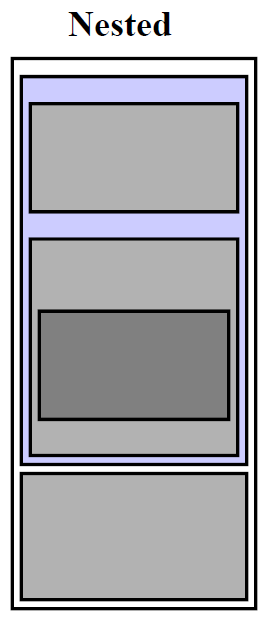
\includegraphics[scale=0.5]{rapport/5/figures/nested_block_structure}
		\end{center}	
		\caption{Illustration of the nested block structure}
		\label{nested_block_structure}
	\end{wrapfigure}


	%INCLUDE BIBLIOGRAPHY!!!	
	\begin{itemize}
	\item No identifier may be declared more than once within the same block (at the same level) %SPO
	\item For any applied occurrence there must be a corresponding occurrence, either within the same block or block which is higher up in the nesting. %SPO
	%INCLUDE BIBL...
	\end{itemize}
	
	
	Referring to figure \ref{nested_block_structure} which demonstrates the functioning of a nested block structure visually. Initially we consider how the nested block structure works in general and later an example of how the nested block structure works in the WAR programming language.
	
	One can have as many and as few blocks as needed, and every sub-block of an existing block, can use all the variables that have been declared in blocks over itself. 
	
	
	%Her kommer noget kode af vores egen for at beskrive hvordan nested block structure virker hos os.
		
\newpage
	
	
%Page 142 i Brown!! :D
		
\subsection{Type rules}
	These are the rules that checks the expressions form, and the type validity.
	
	\subsubsection*{Type rule of $<$}
		$E1 < E2$ is type correct and of type Boolean
		if $E1$ and $E2$ are type correct and of type Integer
	\subsubsection*{Type rule of $>$}
		$E1 > E2$ is type correct and of type Boolean
		if $E1$ and $E2$ are type correct and of type Integer
	\subsubsection*{Type rule of $==$}
		$E1 == E2$ is type correct and of type Boolean
		if $E1$ and $E2$ are type correct and of type Integer
	\subsubsection*{Type rule of $>=$}
		$E1 >= E2$ is type correct and of type Boolean
		if $E1$ and $E2$ are type correct and of type Integer
	\subsubsection*{Type rule of $<=$}
		$E1 <= E2$ is type correct and of type Boolean
		if $E1$ and $E2$ are type correct and of type Integer
	\subsubsection*{Type rule of $while$}
		$while(E){C}$ is type correct
		if $E$ is of type Boolean and $C$ is type correct
	\subsubsection*{Type rule of $if$}
		$if(E){C}$ is type correct
		if $E$ is of type Boolean and $C$ is type correct
	\subsubsection*{Type rule of $else if$}
		$else if(E){C}$ is type correct
		if $E$ is of type Boolean and $C$ is type correct
	\subsubsection*{Type rule of $else$}
		$else{C}$ is type correct
		if $C$ is type correct
	
	\subsubsection*{Type rule of $Position$}
		$Position(I1,I2)$ is type correct and of type Position
		if $I1$ and $I2$ are type correct and of type Integer	
	


%3. Overview of the design choices (Readability, Maintainability, Writeability etc.)(Maybe Tombstone)

%This file only contains inputs!!!
\chapter{Game Description}
	\section{Syntax}
	The first step in writing our interpreter is to make a BNF of our language. BNF stands for {\it Backus Naur form} and is a way of
	structuring the language in a formal way, which will make it easy to implement. A BNF consists of a set of {\it production rules} and each
	production rule consists of: \\
	\begin{itemize}
		 \item Terminals: A {\it terminal } is a literal string that appears in the language in hand.
		 \item Non-terminal: A {\it non-terminal } consists of Non-terminals and Terminals, used for structuring the language.
	\end{itemize}
	
	\subsection*{Production Rule}
		A production rule has the form: \\
		$N ::= X$, \\
		where $X$ is a Non-terminal or a Terminal. \\
		
		The elements in a production rule can be identified by: \\
		Terminals are written in {\bf bold } and 
		Non-terminals are just written in plain text.
	\subsection*{Grouping of production rules}
		If we have two production rules on the form:\\
		$N ::= X$ \\
		$N ::= Y$ \\
		we are allowed to make a transformation: \\
		$N ::= X | Y$ \\
		Meaning $N$ is $X$ or $Y$ \\
	\subsection*{Example of a small BNF}
		\label{ex-bnf}
		\begin{center}
			\begin{tabular}{l l l}
				A		&	::=		&	 AB$ \mid $ B \\
				B		&	::=		&	{\bf b} $\mid$ {\bf n } $\mid$ {\bf f } \\
			\end{tabular}
		\end{center}
		This BNF would allow us to write programs like \\(We use $\rightarrow$ to show applying of a production rule): \\
		{\bf bnf}: A $\rightarrow$ AB $\rightarrow$ A{\bf f} $\rightarrow$ 
		AB{\bf f} $\rightarrow$A{\bf nf} $\rightarrow$ B{\bf nf}$\rightarrow${\bf bnf } \\
	
	\begin{comment}
	
	
	\subsubsection{Terminals}
	
	
		\begin{longtable}[l]{l}
			$\{$\\
			$\}$\\
			$>$\\
			$<$\\
			$($\\
			$)$\\
			$=$\\
			$+$\\
			$-$\\
			$*$\\
			$/$\\
			$\&$\\
			$|$\\
			$"$\\
			$,$\\
			$.$\\
			$;$\\
			$Attack$\\
			$AttackSpeed$\\
			$Behaviour$\\
			$Config$\\
			$Damage$\\
			$Distance$\\
			$else$\\
			$Grid$\\
			$Health$\
			$Height$\\
			$if$\\
			$Maxima$\\
			$Melee$\\
			$MoveAway$\\
			$Movement$\\
			$MoveTowards$\\
			$Position$\\
			$Range$\\
			$Ranged$\\
			$Regiment$\\
			$RegimentPosition$\\
			$Regiments$\\
			$Rules$\\
			$SearchForEnemies$\\
			$SearchForFriends$\\
			$Size$\\
			$Standards$\\
			$Team$\\
			$Teams$\\
			$Type$\\
			$While$\\
			$Width$\\
		\end{longtable}
%	\subsubsection{Nonterminals}
%		\begin{tabular}{l c}
%			Behaviour-Block   & Control-Structure   \\
%			Single-Command    & UnitStat 			\\
%			UnitStat-Name	  & Integer-Literal		\\
%			Comment			  & Team-File 			\\
%			Regiment-Block	  & Expression			\\
%			Operator		  & Config-File			\\
%			Grid-Block	      & Rules-Block 		\\
%			Maximums-Block	  & MaximumsStat		\\
%			MaximumsStat-Name & Standards-Block	 	\\
%			StandardsStat	  & StandardsStat-Name 	\\
%			Identifier		  & 					\\
%		\end{tabular}
\end{comment}
	\subsection{The BNF of the WAR Language}
		{\bf Notes}
		\begin{itemize}
			\item Digit represents one of the digits 0 through 9.
			\item Graphic represents a space or visible character.
			\item Letter represents one of the lower- or upper-case letters 'a','b',.....,or 'z'.
			\item eol represents an end-of-line 'character'.
		\end{itemize}
		\begin{center}
			\begin{longtable}{l l l}
				\endfirsthead
				\endhead
		Team-File					&	::=	&{\bf Team} Identifier Regiment-Block\\
		Identifier					&	::=	&Letter\\
									&$\mid$	&Identifier Digit\\
									&$\mid$	&Identifier Letter\\
		Block-Name					&	::=	&Identifier\\
		Regiment-Block				&	::=	&{\bf Regiment} Block-Name {\bf \{ } UnitStat Behaviour-Block \bf{\} }\\
									&$\mid$	&Regiment-Block {\bf Regiment} Block-Name\\
									&		&{\bf \{ } UnitStat Behaviour-Block \bf{\} }\\
		Behaviour-Block				&	::=	&{\bf Behaviour} Block-Name {\bf \{} Single-Command {\bf \}}  \\
									&$\mid$	& {\bf Behaviour} {\bf = } Block-Name{\bf ;} \\
		Regiment-Declaration			&	::=	&{\bf Regiment} Identifier {\bf =} Regiment-Search{\bf ;}\\
									&$\mid$	&{\bf Regiment} Identifier {\bf =} Block-Name{\bf ;}\\
		Regiment-Search				&	::=	&{\bf SearchForEnemies (}Parameters{\bf)}\\
									&$\mid$	&{\bf SearchForFriends(}Parameters{\bf)}\\
		RegimentStat				&	::=	&Identifier {\bf.} UnitStat-Type \\
		Parameters					&	::=	&UnitStat-Type Operator Integer-Literal\\
		 							&$\mid$	&Parameters{\bf ,} UnitStat-Type Operator Integer-Literal\\
		Single-Command				&	::=	&Control-Structure Single-Command \\
									&$\mid$	&Regiment-Declaration Single-Command\\
									&$\mid$	&UnitFunction Single-command\\
									&$\mid$	&Control-Structure\\
									&$\mid$	&UnitFunction\\
									&$\mid$	&Regiment-Declaration\\
		ElseIf-Structure			&	::=	&{\bf else if( } Expression{\bf )} {\bf \{ } Single-Command {\bf \} } ElseIf-Structure\\
									&$\mid$	&{\bf else if( } Expression{\bf )} {\bf \{ } Single-Command {\bf \} } \\
		Control-Structure			&	::=	&{\bf if( } Expression{\bf )} {\bf \{ } Single-Command {\bf \} }  \\
									&$\mid$	&{\bf if(} Expression {\bf )} {\bf \{ }Single-Command {\bf \}} \\
									&		&{\bf else } {\bf \{ }Single-Command {\bf \} } \\			
									&$\mid$	&{\bf if(} Expression {\bf )} {\bf \{ }Single-Command {\bf \}} \\
									&		&ElseIf-Structure {\bf else } {\bf \{ }Single-Command {\bf \} } \\
									&$\mid$	&{\bf if(} Expression {\bf )} {\bf \{ }Single-Command {\bf \}} ElseIf-Structure \\	
									&$\mid$	&{\bf while (} Expression {\bf )}{\bf \{ } Single-Command {\bf \}} \\
		Expression					&	::=	&Primary-Expression \\
									&$\mid$	&Expression Operator Primary-Expression \\
		Primary-Expression			&	::=	&(Expression)\\
									&$\mid$	&Integer-Literal \\
									&$\mid$	&UnitStat-Type \\
									&$\mid$	&RegimentStat \\
		Operator					&	::=	&$\boldsymbol {+}$\\
									&$\mid$	&$\boldsymbol {-}$\\
									&$\mid$	&$\boldsymbol {*}$\\
									&$\mid$	&$\boldsymbol {/}$\\
									&$\mid$	&$\boldsymbol {<}$\\
									&$\mid$	&$\boldsymbol {>}$\\
									&$\mid$	&$\boldsymbol {<=}$\\
									&$\mid$	&$\boldsymbol {>=}$\\
									&$\mid$	&$\boldsymbol {==}$\\
									&$\mid$	&$\boldsymbol {\&\&}$\\
									&$\mid$	&$\boldsymbol {\|}$\\
		UnitFunction				&	::=	&{\bf Attack(} Identifier {\bf );} \\
									&$\mid$	&{\bf MoveTowards(}Identifier {\bf );} \\
									&$\mid$	&{\bf MoveAway(} Identifier {\bf );} \\
		UnitStat					&	::=	&UnitStat-Declaration UnitStat \\
									&$\mid$	&UnitStat-Declaration \\
		UnitStat-Declaration		&	::=	&{\bf Size =} Integer-Literal{\bf ;} \\
									&$\mid$	&{\bf Type} = AttackType{\bf ;}\\
									&$\mid$	&{\bf  Range =} Integer-Literal{\bf;}\\
									&$\mid$	&{\bf Damage =} Integer-Literal{\bf ;}\\
									&$\mid$	&{\bf Movement = }Integer-Literal{\bf ;} \\				  
									&$\mid$	& {\bf RegimentPosition = Position(} Integer-Literal {\bf ,}\\
									&		& Integer-Literal {\bf );}\\
		UnitStat-Type				&	::=	&{\bf Size}\\
									&$\mid$	&{\bf Type}\\
									&$\mid$	&{\bf Range}\\
									&$\mid$	&{\bf Damage}\\
									&$\mid$	&{\bf Movement}\\
									&$\mid$	&{\bf AttackSpeed}\\
									&$\mid$	&{\bf Health}\\
									&$\mid$	&{\bf Distance}\\
		AttackType					&	::=	&{\bf Melee}\\
									&$\mid$	&{\bf Ranged}\\
		Integer-Literal				&	::=	&Digit\\
									&$\mid$	&Integer-Literal Digit\\
		Comment						&	::=	&{\bf //} Graphic-Literal eol\\
		Graphic-Literal				&	::=	&Graphic Graphic-Literal\\
									&$\mid$	&Graphic\\
		Config-File					&	::=	&{\bf Config} Grid-Block Rules-Block\\
		Grid-Block					&	::=	&{\bf Grid} Block-Name	 {\bf \{} GridStat \bf{\}}\\
		GridStat					&	::=	&GridStat-Declaration GridStat\\
									&$\mid$	&GridStat-Declaration \\
		GridStat-Declaration		&	::=	&{\bf Width = } Integer-Literal;\\
									&$\mid$	&{\bf Height = } Integer-Literal;\\
		Rules-Block					&	::=	&Standards-Block MaximumsBlock\\
		Maximums-Block				&	::=	&{\bf Maximums} {\bf \{} MaximumsStat {\bf \}} \\
		MaximumsStat				&	::=	&MaximumsStat-Declaration MaximumsStat\\
									&$\mid$	&MaximumsStat-Declaration\\
		MaximumsStat-Declaration	&	::=	&{\bf Regiments = } Integer-Literal{\bf ;}\\
									&$\mid$	&{\bf Teams = } Integer-Literal{\bf ;}\\
									&$\mid$	&{\bf Size = } Integer-Literal{\bf ;}\\
									&$\mid$	&{\bf Range = } Integer-Literal{\bf ;}\\
									&$\mid$	&{\bf Damage = } Integer-Literal{\bf ;}\\
									&$\mid$	&{\bf Movement = } Integer-Literal{\bf ;}\\
									&$\mid$	&{\bf AttackSpeed = } Integer-Literal{\bf ;}\\
									&$\mid$	&{\bf Health = } Integer-Literal{\bf ;}\\
		Standards-Block				&	::=	&{\bf Standards} {\bf \{ } UnitStat-Declaration Behaviour-Block\bf{\} }\\
			\end{longtable}
		\end{center}
		
		
	\subsection{EBNF}
		{\it EBNF} stands for {\it Extendend Backus Naur Form} and is, as the name refers to an extension of BNF.
		The EBNF allows us to use regular expressions to express production rules, which makes our rule set more compact and 
		easier to implement.
	
	\subsubsection*{Regular expressions}
		A regular expression is a convenient way of expressing strings. We use the following regular expressions: \\
		\begin{itemize}
			\item *(star): States that the terminal or non-terminal must be used 0 or more times.
			\item Parentheses: Used for grouping of non-terminals and terminals.
			\item $\epsilon$: Represents the empty string.
		\end{itemize}
		Please note that these regular expressions can only be used on the right side of the production rules. \\
		
		By using these regular expression we can \\
		transform the BNF example given in \ref{ex-bnf} to an EBNF: \\
		
		\begin{tabular}{l l l}
			B		&	::=		&	({\bf b} $\mid$ {\bf n } $\mid$ {\bf f })* \\
		\end{tabular}
		
		It's easy to see that the transformation made the rules more compact (we removed one the the production rules), but
		how do we transform a BNF to a EBNF in a systematic way? 
		This can be done by applying {\it left factorization }, {\it elimination of left recursion} and {\it substitution of non-terminals }.
		
		\subsubsection*{Left factorization}
			If we have a production rule on the form: \\
			\begin{tabular}{l l l}
				T		&	::=		&	AB$\mid$AC \\
			\end{tabular}
			
			We can do a left factorization: \\
			\begin{tabular}{l l l}
				T		&	::=		&	A(B$\mid$C) \\
			\end{tabular}
			
			This can be done because T will always start with an A and end with either a B or C.
			
		\subsubsection*{Elimination of left recursion}
			If we have a production rule on the form: \\
			\begin{tabular}{l l l}
				T		&	::=		&	A$\mid$TB \\
			\end{tabular}
			
			We can do an elimination of left recursion: \\
			\begin{tabular}{l l l}
				T		&	::=		&	A(B)* \\
			\end{tabular}
			
			To understand how we can do this look at the first production rule. To terminate the production rule we need 
			to put an A, so T will always consist of an A. When we are not selecting an A(, and terminating) we are only making B's, which is
			the same as B*.
		\subsubsection*{Substitution of non-terminals}
			If we have two production rules on the form: \\
			
			\begin{tabular}{l l l}
				T		&	::=		&	U $\mid$ AUC \\
				U		&	::=		&	{\bf ab} $\mid$ {\bf ba} \\
			\end{tabular} \\
			
			We can do a substitution of the non-terminal U for every production rule. This means that we 
			substitute any occurrence of U in a production rule with what is on the right hand side of U like this: \\
			
			\begin{tabular}{l l l}
				T		&	::=		&	({\bf ab} $\mid$ {\bf ba}) $\mid$ A ({\bf ab} $\mid$ {\bf ba})B \\
			\end{tabular}
	\subsection{The EBNF of the WAR Language}
		Left factorization, substituion of non-terminals 
		and elimination of left recursion was applied to transform the BNF to an EBNF. \\
		
		Substituion of non-terminals have removed the following non-terminals from the BNF: \\
		\begin{itemize}
			\item Else-If
			\item UnitStat
			\item Graphical-Literal
			\item GridStat
			\item MaximumsStat
		\end{itemize}
		
		\begin{center}
			\begin{longtable}{ l l l }
				\endfirsthead
				\endhead
		Team-File					&	::=	&{\bf Team} Identifier Regiment-Block*\\
		Identifier					&	::=	&Letter (Letter $\mid$ Digit)*\\
		Block-Name					&	::=	&Identifier\\
		Regiment-Block				&	::=	&{\bf Regiment} Block-Name {\bf \{ } \\
									&		&UnitStat-Declaration Behaviour-Block \bf{\} }\\
		Behaviour-Block				&	::=	&{\bf Behaviour}(Identifier{\bf \{ }Single-Command \bf{\} } $\mid$ {\bf $=$} Identifier)\\
		Regiment-Declaration		&	::=	&{\bf Regiment} Identifier {\bf =} Regiment-Search{\bf ;}\\
									&$\mid$	&{\bf Regiment} Identifier {\bf =} Block-Name{\bf ;}\\
		Regiment-Search				&	::=	&{\bf SearchForEnemies (} Parameters {\bf )}\\
									&$\mid$	&{\bf SearchForFriends(} Parameters {\bf )}\\
		RegimentStat				&	::=	&Identifier{\bf.}UnitStat-Type \\
		Parameters					&	::=	&UnitStat-Type Operator Integer-Literal\\
									&		&({\bf ,}UnitStat-Type Operator Integer-Literal)*\\
		Single-Command				&	::=	&(Control-Structure $\mid$ UnitFunction $\mid$ Regiment-Declaration)*\\
									&		&(Control-Structure $\mid$ UnitFunction $\mid$ Regiment-Declaration)\\		
		Control-Structure			&	::=	&if(Expression) \bf{\{}Single-Command \bf{\}}\\
									&		&(\bf{else if(}Expression\bf{)\{ }Single-Command\bf{ \}})* \\
									&		&($\epsilon$ $\mid$ else \bf{\{ }Single-Command \bf{\} }\\					   
									&$\mid$	&while(Expression)\bf{\{ } Single-Command \bf{\}}\\
		Expression					&	::=	&Primary-Expression (Operator Primary-Expression)*\\
		Primary-Expression			&	::=	&(Expression)\\
									&$\mid$	&Integer-Literal \\
									&$\mid$	&UnitStat-Type\\
									&$\mid$	&RegimentStat \\	
		Operator					&	::=	&$\boldsymbol {+}$\\
									&$\mid$	&$\boldsymbol {-}$\\
									&$\mid$	&$\boldsymbol {*}$\\
									&$\mid$	&$\boldsymbol {/}$\\
									&$\mid$	&$\boldsymbol {<}$\\
									&$\mid$	&$\boldsymbol {>}$\\
									&$\mid$	&$\boldsymbol {<=}$\\
									&$\mid$	&$\boldsymbol {>=}$\\
									&$\mid$	&$\boldsymbol {==}$\\
									&$\mid$	&$\boldsymbol {\&\&}$\\
									&$\mid$	&$\boldsymbol {\|}$\\
		UnitFunction				&	::=	&({\bf Attack} $\mid$ {\bf MoveTowards} $\mid${\bf MoveAway}){\bf (} Identifier {\bf );}\\
		UnitStat-Declaration		&	::=	&({\bf Size}$\mid${\bf Range}$\mid${\bf Damage} $\mid${\bf Movement}\\ 
									&		&$\mid$ {\bf AttackSpeed}$\mid${\bf Health}) ${\bf = }$ Integer-Literal{\bf ;} \\
									&$\mid$	&{\bf RegimentPosition =} \\
									&		&{\bf Position(}Integer-Literal{\bf ,}Integer-Literal{\bf );}\\
									&$\mid$	&{\bf Type} = AttackType{\bf ;}\\
		UnitStat-Type				&	::=	&({\bf Size}$\mid${\bf Range}$\mid${\bf Damage} $\mid$\\
									&		&{\bf Movement}$\mid$ {\bf AttackSpeed}$\mid${\bf Health}$\mid${\bf Distance})\\ 
		AttackType					&	::=	&{\bf Melee} $\mid$ {\bf Ranged} \\
		Integer-Literal				&	::=	&Digit Digit*\\
		Comment						&	::=	&{\bf //} Graphic* eol\\
		Config-File					&	::=	&{\bf Config} Grid-Block Rules-Block  		\\
		Grid-Block					&	::=	&{\bf Grid} Block-Name	 {\bf \{} GridStat-Declaration* \bf{\}} \\
		GridStat-Declaration		&	::=	&({\bf Width} $\mid$ {\bf Height})=  Integer-Literal{\bf ;} \\	
		Rules-Block					&	::=	&Standards-Block MaximumsBlock 				\\
		Maximums-Block				&	::=	&{\bf Maximums} {\bf \{} (MaximumsStat-Declaration)* {\bf \}}\\
		MaximumsStat-Declaration	&	::=	&({\bf Regiments }$\mid${\bf Teams}$\mid${\bf Size}$\mid$\\
									&		&{\bf Range}$\mid${\bf Damage}$\mid${\bf Movement}$\mid$\\
									&		&{\bf AttackSpeed}$\mid${\bf Health}) =  Integer-Literal{\bf ;}\\
		Standards-Block				&	::=	&{\bf Standards} {\bf \{ } UnitStat-Declaration* Behaviour-Block\bf{\} }		\\
			\end{longtable}
		\end{center}					     

	\section{Construction of the parser}
	In this section we will describe how one can construct a parser from a EBNF, but first we will describe how a parser is and how it works.
	
	\subsection{Parsing}
		The job of a parser is to check if a program is correct and 
		to determine the structure of the program, usually done by constructing tree structure.
		There are two ways of checking this {\it Bottom-up Parsing} and {\it Top-Down Parsing}.
		
		\subsubsection*{Bottom-up Parsing}
			This way of parsing takes simple structures and combining them to more complex structures.
			We show how this type of parsing works by applying Bottom-up parsing on this code written in : \\
			{\bf Maximums \{ Regiments = 5;\} }
			
			\begin{enumerate}
				\item Looks at 5 - Identifies it as an Integer-literal
				\item Looks at 5* -
			\end{enumerate}
			
	\section{Semantics}
\label{sec:conanal}
This section will define the scope and type rules of WAR.
	\subsection{Scope rules}
		A scope is a block of code, in WAR one is able to denote a new scope by using $\{$ to start the scope and $\}$.
		A scope placed inside another scope is called a {\it nested scope}. A {\it scope level} denotes how nested a given scope is,
		e.g. identifiers at scope level 0 is outside any scope, identifiers at scope level 1 is inside one scope etc.
		\begin{lstlisting}
		Scope
		{
			//Scope level 1
			identifier = 2
			Scope
			{
				//Scope level 2
				identifier = 2
			}
		}
		\end{lstlisting}
		
		Scope rules dictate the accessibility of identifiers from one scope to another.
	
	%These are the rules that defines how the identifiers must be read, and where to declare them - also known as identification.
	The WAR language has a nested block-structure which means we may have constants or variables can be defined in multiple scope levels. 
	Scope rules may be defined in levels, such that a declaration in the outermost block is at scope level 1, however, since the language has no declaration of variables, only constants, it works the same way. If you declare the $Size$ of a regiment at scope level 1, you can use $Size$ in all the higher scope levels. Declarations inside a block are referred to as being local in that block.

	The use of a nested block structure we follow some basic scope rules:
	\begin{wrapfigure}{r}{0.5\textwidth}
		\begin{center}
			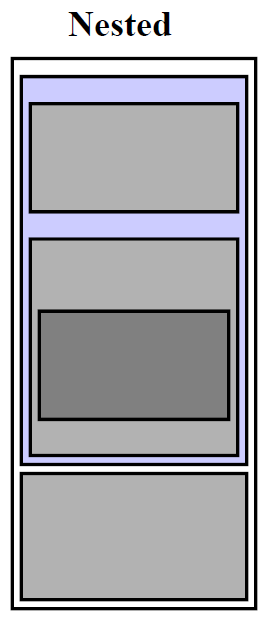
\includegraphics[scale=0.5]{rapport/5/figures/nested_block_structure}
		\end{center}	
		\caption{Illustration of the nested block structure}
		\label{nested_block_structure}
	\end{wrapfigure}


	%INCLUDE BIBLIOGRAPHY!!!	
	\begin{itemize}
	\item No identifier may be declared more than once within the same block (at the same level) %SPO
	\item For any applied occurrence there must be a corresponding occurrence, either within the same block or block which is higher up in the nesting. %SPO
	%INCLUDE BIBL...
	\end{itemize}
	
	
	Referring to figure \ref{nested_block_structure} which demonstrates the functioning of a nested block structure visually. Initially we consider how the nested block structure works in general and later an example of how the nested block structure works in the WAR programming language.
	
	One can have as many and as few blocks as needed, and every sub-block of an existing block, can use all the variables that have been declared in blocks over itself. 
	
	
	%Her kommer noget kode af vores egen for at beskrive hvordan nested block structure virker hos os.
		
\newpage
	
	
%Page 142 i Brown!! :D
		
\subsection{Type rules}
	These are the rules that checks the expressions form, and the type validity.
	
	\subsubsection*{Type rule of $<$}
		$E1 < E2$ is type correct and of type Boolean
		if $E1$ and $E2$ are type correct and of type Integer
	\subsubsection*{Type rule of $>$}
		$E1 > E2$ is type correct and of type Boolean
		if $E1$ and $E2$ are type correct and of type Integer
	\subsubsection*{Type rule of $==$}
		$E1 == E2$ is type correct and of type Boolean
		if $E1$ and $E2$ are type correct and of type Integer
	\subsubsection*{Type rule of $>=$}
		$E1 >= E2$ is type correct and of type Boolean
		if $E1$ and $E2$ are type correct and of type Integer
	\subsubsection*{Type rule of $<=$}
		$E1 <= E2$ is type correct and of type Boolean
		if $E1$ and $E2$ are type correct and of type Integer
	\subsubsection*{Type rule of $while$}
		$while(E){C}$ is type correct
		if $E$ is of type Boolean and $C$ is type correct
	\subsubsection*{Type rule of $if$}
		$if(E){C}$ is type correct
		if $E$ is of type Boolean and $C$ is type correct
	\subsubsection*{Type rule of $else if$}
		$else if(E){C}$ is type correct
		if $E$ is of type Boolean and $C$ is type correct
	\subsubsection*{Type rule of $else$}
		$else{C}$ is type correct
		if $C$ is type correct
	
	\subsubsection*{Type rule of $Position$}
		$Position(I1,I2)$ is type correct and of type Position
		if $I1$ and $I2$ are type correct and of type Integer	
	


%4. Language documentation (simple, what you can do, and what you can?t do - how to use the language) - Like Java Documentation.

%This file only contains inputs!!!
\chapter{Game Description}
	\section{Syntax}
	The first step in writing our interpreter is to make a BNF of our language. BNF stands for {\it Backus Naur form} and is a way of
	structuring the language in a formal way, which will make it easy to implement. A BNF consists of a set of {\it production rules} and each
	production rule consists of: \\
	\begin{itemize}
		 \item Terminals: A {\it terminal } is a literal string that appears in the language in hand.
		 \item Non-terminal: A {\it non-terminal } consists of Non-terminals and Terminals, used for structuring the language.
	\end{itemize}
	
	\subsection*{Production Rule}
		A production rule has the form: \\
		$N ::= X$, \\
		where $X$ is a Non-terminal or a Terminal. \\
		
		The elements in a production rule can be identified by: \\
		Terminals are written in {\bf bold } and 
		Non-terminals are just written in plain text.
	\subsection*{Grouping of production rules}
		If we have two production rules on the form:\\
		$N ::= X$ \\
		$N ::= Y$ \\
		we are allowed to make a transformation: \\
		$N ::= X | Y$ \\
		Meaning $N$ is $X$ or $Y$ \\
	\subsection*{Example of a small BNF}
		\label{ex-bnf}
		\begin{center}
			\begin{tabular}{l l l}
				A		&	::=		&	 AB$ \mid $ B \\
				B		&	::=		&	{\bf b} $\mid$ {\bf n } $\mid$ {\bf f } \\
			\end{tabular}
		\end{center}
		This BNF would allow us to write programs like \\(We use $\rightarrow$ to show applying of a production rule): \\
		{\bf bnf}: A $\rightarrow$ AB $\rightarrow$ A{\bf f} $\rightarrow$ 
		AB{\bf f} $\rightarrow$A{\bf nf} $\rightarrow$ B{\bf nf}$\rightarrow${\bf bnf } \\
	
	\begin{comment}
	
	
	\subsubsection{Terminals}
	
	
		\begin{longtable}[l]{l}
			$\{$\\
			$\}$\\
			$>$\\
			$<$\\
			$($\\
			$)$\\
			$=$\\
			$+$\\
			$-$\\
			$*$\\
			$/$\\
			$\&$\\
			$|$\\
			$"$\\
			$,$\\
			$.$\\
			$;$\\
			$Attack$\\
			$AttackSpeed$\\
			$Behaviour$\\
			$Config$\\
			$Damage$\\
			$Distance$\\
			$else$\\
			$Grid$\\
			$Health$\
			$Height$\\
			$if$\\
			$Maxima$\\
			$Melee$\\
			$MoveAway$\\
			$Movement$\\
			$MoveTowards$\\
			$Position$\\
			$Range$\\
			$Ranged$\\
			$Regiment$\\
			$RegimentPosition$\\
			$Regiments$\\
			$Rules$\\
			$SearchForEnemies$\\
			$SearchForFriends$\\
			$Size$\\
			$Standards$\\
			$Team$\\
			$Teams$\\
			$Type$\\
			$While$\\
			$Width$\\
		\end{longtable}
%	\subsubsection{Nonterminals}
%		\begin{tabular}{l c}
%			Behaviour-Block   & Control-Structure   \\
%			Single-Command    & UnitStat 			\\
%			UnitStat-Name	  & Integer-Literal		\\
%			Comment			  & Team-File 			\\
%			Regiment-Block	  & Expression			\\
%			Operator		  & Config-File			\\
%			Grid-Block	      & Rules-Block 		\\
%			Maximums-Block	  & MaximumsStat		\\
%			MaximumsStat-Name & Standards-Block	 	\\
%			StandardsStat	  & StandardsStat-Name 	\\
%			Identifier		  & 					\\
%		\end{tabular}
\end{comment}
	\subsection{The BNF of the WAR Language}
		{\bf Notes}
		\begin{itemize}
			\item Digit represents one of the digits 0 through 9.
			\item Graphic represents a space or visible character.
			\item Letter represents one of the lower- or upper-case letters 'a','b',.....,or 'z'.
			\item eol represents an end-of-line 'character'.
		\end{itemize}
		\begin{center}
			\begin{longtable}{l l l}
				\endfirsthead
				\endhead
		Team-File					&	::=	&{\bf Team} Identifier Regiment-Block\\
		Identifier					&	::=	&Letter\\
									&$\mid$	&Identifier Digit\\
									&$\mid$	&Identifier Letter\\
		Block-Name					&	::=	&Identifier\\
		Regiment-Block				&	::=	&{\bf Regiment} Block-Name {\bf \{ } UnitStat Behaviour-Block \bf{\} }\\
									&$\mid$	&Regiment-Block {\bf Regiment} Block-Name\\
									&		&{\bf \{ } UnitStat Behaviour-Block \bf{\} }\\
		Behaviour-Block				&	::=	&{\bf Behaviour} Block-Name {\bf \{} Single-Command {\bf \}}  \\
									&$\mid$	& {\bf Behaviour} {\bf = } Block-Name{\bf ;} \\
		Regiment-Declaration			&	::=	&{\bf Regiment} Identifier {\bf =} Regiment-Search{\bf ;}\\
									&$\mid$	&{\bf Regiment} Identifier {\bf =} Block-Name{\bf ;}\\
		Regiment-Search				&	::=	&{\bf SearchForEnemies (}Parameters{\bf)}\\
									&$\mid$	&{\bf SearchForFriends(}Parameters{\bf)}\\
		RegimentStat				&	::=	&Identifier {\bf.} UnitStat-Type \\
		Parameters					&	::=	&UnitStat-Type Operator Integer-Literal\\
		 							&$\mid$	&Parameters{\bf ,} UnitStat-Type Operator Integer-Literal\\
		Single-Command				&	::=	&Control-Structure Single-Command \\
									&$\mid$	&Regiment-Declaration Single-Command\\
									&$\mid$	&UnitFunction Single-command\\
									&$\mid$	&Control-Structure\\
									&$\mid$	&UnitFunction\\
									&$\mid$	&Regiment-Declaration\\
		ElseIf-Structure			&	::=	&{\bf else if( } Expression{\bf )} {\bf \{ } Single-Command {\bf \} } ElseIf-Structure\\
									&$\mid$	&{\bf else if( } Expression{\bf )} {\bf \{ } Single-Command {\bf \} } \\
		Control-Structure			&	::=	&{\bf if( } Expression{\bf )} {\bf \{ } Single-Command {\bf \} }  \\
									&$\mid$	&{\bf if(} Expression {\bf )} {\bf \{ }Single-Command {\bf \}} \\
									&		&{\bf else } {\bf \{ }Single-Command {\bf \} } \\			
									&$\mid$	&{\bf if(} Expression {\bf )} {\bf \{ }Single-Command {\bf \}} \\
									&		&ElseIf-Structure {\bf else } {\bf \{ }Single-Command {\bf \} } \\
									&$\mid$	&{\bf if(} Expression {\bf )} {\bf \{ }Single-Command {\bf \}} ElseIf-Structure \\	
									&$\mid$	&{\bf while (} Expression {\bf )}{\bf \{ } Single-Command {\bf \}} \\
		Expression					&	::=	&Primary-Expression \\
									&$\mid$	&Expression Operator Primary-Expression \\
		Primary-Expression			&	::=	&(Expression)\\
									&$\mid$	&Integer-Literal \\
									&$\mid$	&UnitStat-Type \\
									&$\mid$	&RegimentStat \\
		Operator					&	::=	&$\boldsymbol {+}$\\
									&$\mid$	&$\boldsymbol {-}$\\
									&$\mid$	&$\boldsymbol {*}$\\
									&$\mid$	&$\boldsymbol {/}$\\
									&$\mid$	&$\boldsymbol {<}$\\
									&$\mid$	&$\boldsymbol {>}$\\
									&$\mid$	&$\boldsymbol {<=}$\\
									&$\mid$	&$\boldsymbol {>=}$\\
									&$\mid$	&$\boldsymbol {==}$\\
									&$\mid$	&$\boldsymbol {\&\&}$\\
									&$\mid$	&$\boldsymbol {\|}$\\
		UnitFunction				&	::=	&{\bf Attack(} Identifier {\bf );} \\
									&$\mid$	&{\bf MoveTowards(}Identifier {\bf );} \\
									&$\mid$	&{\bf MoveAway(} Identifier {\bf );} \\
		UnitStat					&	::=	&UnitStat-Declaration UnitStat \\
									&$\mid$	&UnitStat-Declaration \\
		UnitStat-Declaration		&	::=	&{\bf Size =} Integer-Literal{\bf ;} \\
									&$\mid$	&{\bf Type} = AttackType{\bf ;}\\
									&$\mid$	&{\bf  Range =} Integer-Literal{\bf;}\\
									&$\mid$	&{\bf Damage =} Integer-Literal{\bf ;}\\
									&$\mid$	&{\bf Movement = }Integer-Literal{\bf ;} \\				  
									&$\mid$	& {\bf RegimentPosition = Position(} Integer-Literal {\bf ,}\\
									&		& Integer-Literal {\bf );}\\
		UnitStat-Type				&	::=	&{\bf Size}\\
									&$\mid$	&{\bf Type}\\
									&$\mid$	&{\bf Range}\\
									&$\mid$	&{\bf Damage}\\
									&$\mid$	&{\bf Movement}\\
									&$\mid$	&{\bf AttackSpeed}\\
									&$\mid$	&{\bf Health}\\
									&$\mid$	&{\bf Distance}\\
		AttackType					&	::=	&{\bf Melee}\\
									&$\mid$	&{\bf Ranged}\\
		Integer-Literal				&	::=	&Digit\\
									&$\mid$	&Integer-Literal Digit\\
		Comment						&	::=	&{\bf //} Graphic-Literal eol\\
		Graphic-Literal				&	::=	&Graphic Graphic-Literal\\
									&$\mid$	&Graphic\\
		Config-File					&	::=	&{\bf Config} Grid-Block Rules-Block\\
		Grid-Block					&	::=	&{\bf Grid} Block-Name	 {\bf \{} GridStat \bf{\}}\\
		GridStat					&	::=	&GridStat-Declaration GridStat\\
									&$\mid$	&GridStat-Declaration \\
		GridStat-Declaration		&	::=	&{\bf Width = } Integer-Literal;\\
									&$\mid$	&{\bf Height = } Integer-Literal;\\
		Rules-Block					&	::=	&Standards-Block MaximumsBlock\\
		Maximums-Block				&	::=	&{\bf Maximums} {\bf \{} MaximumsStat {\bf \}} \\
		MaximumsStat				&	::=	&MaximumsStat-Declaration MaximumsStat\\
									&$\mid$	&MaximumsStat-Declaration\\
		MaximumsStat-Declaration	&	::=	&{\bf Regiments = } Integer-Literal{\bf ;}\\
									&$\mid$	&{\bf Teams = } Integer-Literal{\bf ;}\\
									&$\mid$	&{\bf Size = } Integer-Literal{\bf ;}\\
									&$\mid$	&{\bf Range = } Integer-Literal{\bf ;}\\
									&$\mid$	&{\bf Damage = } Integer-Literal{\bf ;}\\
									&$\mid$	&{\bf Movement = } Integer-Literal{\bf ;}\\
									&$\mid$	&{\bf AttackSpeed = } Integer-Literal{\bf ;}\\
									&$\mid$	&{\bf Health = } Integer-Literal{\bf ;}\\
		Standards-Block				&	::=	&{\bf Standards} {\bf \{ } UnitStat-Declaration Behaviour-Block\bf{\} }\\
			\end{longtable}
		\end{center}
		
		
	\subsection{EBNF}
		{\it EBNF} stands for {\it Extendend Backus Naur Form} and is, as the name refers to an extension of BNF.
		The EBNF allows us to use regular expressions to express production rules, which makes our rule set more compact and 
		easier to implement.
	
	\subsubsection*{Regular expressions}
		A regular expression is a convenient way of expressing strings. We use the following regular expressions: \\
		\begin{itemize}
			\item *(star): States that the terminal or non-terminal must be used 0 or more times.
			\item Parentheses: Used for grouping of non-terminals and terminals.
			\item $\epsilon$: Represents the empty string.
		\end{itemize}
		Please note that these regular expressions can only be used on the right side of the production rules. \\
		
		By using these regular expression we can \\
		transform the BNF example given in \ref{ex-bnf} to an EBNF: \\
		
		\begin{tabular}{l l l}
			B		&	::=		&	({\bf b} $\mid$ {\bf n } $\mid$ {\bf f })* \\
		\end{tabular}
		
		It's easy to see that the transformation made the rules more compact (we removed one the the production rules), but
		how do we transform a BNF to a EBNF in a systematic way? 
		This can be done by applying {\it left factorization }, {\it elimination of left recursion} and {\it substitution of non-terminals }.
		
		\subsubsection*{Left factorization}
			If we have a production rule on the form: \\
			\begin{tabular}{l l l}
				T		&	::=		&	AB$\mid$AC \\
			\end{tabular}
			
			We can do a left factorization: \\
			\begin{tabular}{l l l}
				T		&	::=		&	A(B$\mid$C) \\
			\end{tabular}
			
			This can be done because T will always start with an A and end with either a B or C.
			
		\subsubsection*{Elimination of left recursion}
			If we have a production rule on the form: \\
			\begin{tabular}{l l l}
				T		&	::=		&	A$\mid$TB \\
			\end{tabular}
			
			We can do an elimination of left recursion: \\
			\begin{tabular}{l l l}
				T		&	::=		&	A(B)* \\
			\end{tabular}
			
			To understand how we can do this look at the first production rule. To terminate the production rule we need 
			to put an A, so T will always consist of an A. When we are not selecting an A(, and terminating) we are only making B's, which is
			the same as B*.
		\subsubsection*{Substitution of non-terminals}
			If we have two production rules on the form: \\
			
			\begin{tabular}{l l l}
				T		&	::=		&	U $\mid$ AUC \\
				U		&	::=		&	{\bf ab} $\mid$ {\bf ba} \\
			\end{tabular} \\
			
			We can do a substitution of the non-terminal U for every production rule. This means that we 
			substitute any occurrence of U in a production rule with what is on the right hand side of U like this: \\
			
			\begin{tabular}{l l l}
				T		&	::=		&	({\bf ab} $\mid$ {\bf ba}) $\mid$ A ({\bf ab} $\mid$ {\bf ba})B \\
			\end{tabular}
	\subsection{The EBNF of the WAR Language}
		Left factorization, substituion of non-terminals 
		and elimination of left recursion was applied to transform the BNF to an EBNF. \\
		
		Substituion of non-terminals have removed the following non-terminals from the BNF: \\
		\begin{itemize}
			\item Else-If
			\item UnitStat
			\item Graphical-Literal
			\item GridStat
			\item MaximumsStat
		\end{itemize}
		
		\begin{center}
			\begin{longtable}{ l l l }
				\endfirsthead
				\endhead
		Team-File					&	::=	&{\bf Team} Identifier Regiment-Block*\\
		Identifier					&	::=	&Letter (Letter $\mid$ Digit)*\\
		Block-Name					&	::=	&Identifier\\
		Regiment-Block				&	::=	&{\bf Regiment} Block-Name {\bf \{ } \\
									&		&UnitStat-Declaration Behaviour-Block \bf{\} }\\
		Behaviour-Block				&	::=	&{\bf Behaviour}(Identifier{\bf \{ }Single-Command \bf{\} } $\mid$ {\bf $=$} Identifier)\\
		Regiment-Declaration		&	::=	&{\bf Regiment} Identifier {\bf =} Regiment-Search{\bf ;}\\
									&$\mid$	&{\bf Regiment} Identifier {\bf =} Block-Name{\bf ;}\\
		Regiment-Search				&	::=	&{\bf SearchForEnemies (} Parameters {\bf )}\\
									&$\mid$	&{\bf SearchForFriends(} Parameters {\bf )}\\
		RegimentStat				&	::=	&Identifier{\bf.}UnitStat-Type \\
		Parameters					&	::=	&UnitStat-Type Operator Integer-Literal\\
									&		&({\bf ,}UnitStat-Type Operator Integer-Literal)*\\
		Single-Command				&	::=	&(Control-Structure $\mid$ UnitFunction $\mid$ Regiment-Declaration)*\\
									&		&(Control-Structure $\mid$ UnitFunction $\mid$ Regiment-Declaration)\\		
		Control-Structure			&	::=	&if(Expression) \bf{\{}Single-Command \bf{\}}\\
									&		&(\bf{else if(}Expression\bf{)\{ }Single-Command\bf{ \}})* \\
									&		&($\epsilon$ $\mid$ else \bf{\{ }Single-Command \bf{\} }\\					   
									&$\mid$	&while(Expression)\bf{\{ } Single-Command \bf{\}}\\
		Expression					&	::=	&Primary-Expression (Operator Primary-Expression)*\\
		Primary-Expression			&	::=	&(Expression)\\
									&$\mid$	&Integer-Literal \\
									&$\mid$	&UnitStat-Type\\
									&$\mid$	&RegimentStat \\	
		Operator					&	::=	&$\boldsymbol {+}$\\
									&$\mid$	&$\boldsymbol {-}$\\
									&$\mid$	&$\boldsymbol {*}$\\
									&$\mid$	&$\boldsymbol {/}$\\
									&$\mid$	&$\boldsymbol {<}$\\
									&$\mid$	&$\boldsymbol {>}$\\
									&$\mid$	&$\boldsymbol {<=}$\\
									&$\mid$	&$\boldsymbol {>=}$\\
									&$\mid$	&$\boldsymbol {==}$\\
									&$\mid$	&$\boldsymbol {\&\&}$\\
									&$\mid$	&$\boldsymbol {\|}$\\
		UnitFunction				&	::=	&({\bf Attack} $\mid$ {\bf MoveTowards} $\mid${\bf MoveAway}){\bf (} Identifier {\bf );}\\
		UnitStat-Declaration		&	::=	&({\bf Size}$\mid${\bf Range}$\mid${\bf Damage} $\mid${\bf Movement}\\ 
									&		&$\mid$ {\bf AttackSpeed}$\mid${\bf Health}) ${\bf = }$ Integer-Literal{\bf ;} \\
									&$\mid$	&{\bf RegimentPosition =} \\
									&		&{\bf Position(}Integer-Literal{\bf ,}Integer-Literal{\bf );}\\
									&$\mid$	&{\bf Type} = AttackType{\bf ;}\\
		UnitStat-Type				&	::=	&({\bf Size}$\mid${\bf Range}$\mid${\bf Damage} $\mid$\\
									&		&{\bf Movement}$\mid$ {\bf AttackSpeed}$\mid${\bf Health}$\mid${\bf Distance})\\ 
		AttackType					&	::=	&{\bf Melee} $\mid$ {\bf Ranged} \\
		Integer-Literal				&	::=	&Digit Digit*\\
		Comment						&	::=	&{\bf //} Graphic* eol\\
		Config-File					&	::=	&{\bf Config} Grid-Block Rules-Block  		\\
		Grid-Block					&	::=	&{\bf Grid} Block-Name	 {\bf \{} GridStat-Declaration* \bf{\}} \\
		GridStat-Declaration		&	::=	&({\bf Width} $\mid$ {\bf Height})=  Integer-Literal{\bf ;} \\	
		Rules-Block					&	::=	&Standards-Block MaximumsBlock 				\\
		Maximums-Block				&	::=	&{\bf Maximums} {\bf \{} (MaximumsStat-Declaration)* {\bf \}}\\
		MaximumsStat-Declaration	&	::=	&({\bf Regiments }$\mid${\bf Teams}$\mid${\bf Size}$\mid$\\
									&		&{\bf Range}$\mid${\bf Damage}$\mid${\bf Movement}$\mid$\\
									&		&{\bf AttackSpeed}$\mid${\bf Health}) =  Integer-Literal{\bf ;}\\
		Standards-Block				&	::=	&{\bf Standards} {\bf \{ } UnitStat-Declaration* Behaviour-Block\bf{\} }		\\
			\end{longtable}
		\end{center}					     

	\section{Construction of the parser}
	In this section we will describe how one can construct a parser from a EBNF, but first we will describe how a parser is and how it works.
	
	\subsection{Parsing}
		The job of a parser is to check if a program is correct and 
		to determine the structure of the program, usually done by constructing tree structure.
		There are two ways of checking this {\it Bottom-up Parsing} and {\it Top-Down Parsing}.
		
		\subsubsection*{Bottom-up Parsing}
			This way of parsing takes simple structures and combining them to more complex structures.
			We show how this type of parsing works by applying Bottom-up parsing on this code written in : \\
			{\bf Maximums \{ Regiments = 5;\} }
			
			\begin{enumerate}
				\item Looks at 5 - Identifies it as an Integer-literal
				\item Looks at 5* -
			\end{enumerate}
			
	\section{Semantics}
\label{sec:conanal}
This section will define the scope and type rules of WAR.
	\subsection{Scope rules}
		A scope is a block of code, in WAR one is able to denote a new scope by using $\{$ to start the scope and $\}$.
		A scope placed inside another scope is called a {\it nested scope}. A {\it scope level} denotes how nested a given scope is,
		e.g. identifiers at scope level 0 is outside any scope, identifiers at scope level 1 is inside one scope etc.
		\begin{lstlisting}
		Scope
		{
			//Scope level 1
			identifier = 2
			Scope
			{
				//Scope level 2
				identifier = 2
			}
		}
		\end{lstlisting}
		
		Scope rules dictate the accessibility of identifiers from one scope to another.
	
	%These are the rules that defines how the identifiers must be read, and where to declare them - also known as identification.
	The WAR language has a nested block-structure which means we may have constants or variables can be defined in multiple scope levels. 
	Scope rules may be defined in levels, such that a declaration in the outermost block is at scope level 1, however, since the language has no declaration of variables, only constants, it works the same way. If you declare the $Size$ of a regiment at scope level 1, you can use $Size$ in all the higher scope levels. Declarations inside a block are referred to as being local in that block.

	The use of a nested block structure we follow some basic scope rules:
	\begin{wrapfigure}{r}{0.5\textwidth}
		\begin{center}
			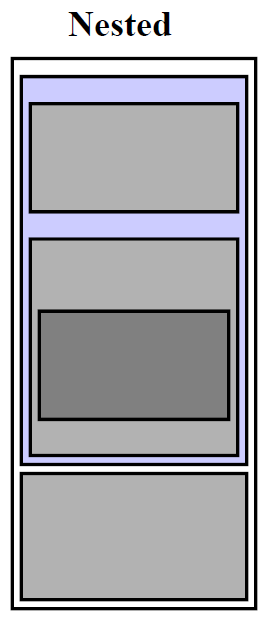
\includegraphics[scale=0.5]{rapport/5/figures/nested_block_structure}
		\end{center}	
		\caption{Illustration of the nested block structure}
		\label{nested_block_structure}
	\end{wrapfigure}


	%INCLUDE BIBLIOGRAPHY!!!	
	\begin{itemize}
	\item No identifier may be declared more than once within the same block (at the same level) %SPO
	\item For any applied occurrence there must be a corresponding occurrence, either within the same block or block which is higher up in the nesting. %SPO
	%INCLUDE BIBL...
	\end{itemize}
	
	
	Referring to figure \ref{nested_block_structure} which demonstrates the functioning of a nested block structure visually. Initially we consider how the nested block structure works in general and later an example of how the nested block structure works in the WAR programming language.
	
	One can have as many and as few blocks as needed, and every sub-block of an existing block, can use all the variables that have been declared in blocks over itself. 
	
	
	%Her kommer noget kode af vores egen for at beskrive hvordan nested block structure virker hos os.
		
\newpage
	
	
%Page 142 i Brown!! :D
		
\subsection{Type rules}
	These are the rules that checks the expressions form, and the type validity.
	
	\subsubsection*{Type rule of $<$}
		$E1 < E2$ is type correct and of type Boolean
		if $E1$ and $E2$ are type correct and of type Integer
	\subsubsection*{Type rule of $>$}
		$E1 > E2$ is type correct and of type Boolean
		if $E1$ and $E2$ are type correct and of type Integer
	\subsubsection*{Type rule of $==$}
		$E1 == E2$ is type correct and of type Boolean
		if $E1$ and $E2$ are type correct and of type Integer
	\subsubsection*{Type rule of $>=$}
		$E1 >= E2$ is type correct and of type Boolean
		if $E1$ and $E2$ are type correct and of type Integer
	\subsubsection*{Type rule of $<=$}
		$E1 <= E2$ is type correct and of type Boolean
		if $E1$ and $E2$ are type correct and of type Integer
	\subsubsection*{Type rule of $while$}
		$while(E){C}$ is type correct
		if $E$ is of type Boolean and $C$ is type correct
	\subsubsection*{Type rule of $if$}
		$if(E){C}$ is type correct
		if $E$ is of type Boolean and $C$ is type correct
	\subsubsection*{Type rule of $else if$}
		$else if(E){C}$ is type correct
		if $E$ is of type Boolean and $C$ is type correct
	\subsubsection*{Type rule of $else$}
		$else{C}$ is type correct
		if $C$ is type correct
	
	\subsubsection*{Type rule of $Position$}
		$Position(I1,I2)$ is type correct and of type Position
		if $I1$ and $I2$ are type correct and of type Integer	
	


%5. The actual design of the language, BNF, EBNF, Contextual analysis.

%This file only contains inputs!!!
\chapter{Game Description}
	\section{Syntax}
	The first step in writing our interpreter is to make a BNF of our language. BNF stands for {\it Backus Naur form} and is a way of
	structuring the language in a formal way, which will make it easy to implement. A BNF consists of a set of {\it production rules} and each
	production rule consists of: \\
	\begin{itemize}
		 \item Terminals: A {\it terminal } is a literal string that appears in the language in hand.
		 \item Non-terminal: A {\it non-terminal } consists of Non-terminals and Terminals, used for structuring the language.
	\end{itemize}
	
	\subsection*{Production Rule}
		A production rule has the form: \\
		$N ::= X$, \\
		where $X$ is a Non-terminal or a Terminal. \\
		
		The elements in a production rule can be identified by: \\
		Terminals are written in {\bf bold } and 
		Non-terminals are just written in plain text.
	\subsection*{Grouping of production rules}
		If we have two production rules on the form:\\
		$N ::= X$ \\
		$N ::= Y$ \\
		we are allowed to make a transformation: \\
		$N ::= X | Y$ \\
		Meaning $N$ is $X$ or $Y$ \\
	\subsection*{Example of a small BNF}
		\label{ex-bnf}
		\begin{center}
			\begin{tabular}{l l l}
				A		&	::=		&	 AB$ \mid $ B \\
				B		&	::=		&	{\bf b} $\mid$ {\bf n } $\mid$ {\bf f } \\
			\end{tabular}
		\end{center}
		This BNF would allow us to write programs like \\(We use $\rightarrow$ to show applying of a production rule): \\
		{\bf bnf}: A $\rightarrow$ AB $\rightarrow$ A{\bf f} $\rightarrow$ 
		AB{\bf f} $\rightarrow$A{\bf nf} $\rightarrow$ B{\bf nf}$\rightarrow${\bf bnf } \\
	
	\begin{comment}
	
	
	\subsubsection{Terminals}
	
	
		\begin{longtable}[l]{l}
			$\{$\\
			$\}$\\
			$>$\\
			$<$\\
			$($\\
			$)$\\
			$=$\\
			$+$\\
			$-$\\
			$*$\\
			$/$\\
			$\&$\\
			$|$\\
			$"$\\
			$,$\\
			$.$\\
			$;$\\
			$Attack$\\
			$AttackSpeed$\\
			$Behaviour$\\
			$Config$\\
			$Damage$\\
			$Distance$\\
			$else$\\
			$Grid$\\
			$Health$\
			$Height$\\
			$if$\\
			$Maxima$\\
			$Melee$\\
			$MoveAway$\\
			$Movement$\\
			$MoveTowards$\\
			$Position$\\
			$Range$\\
			$Ranged$\\
			$Regiment$\\
			$RegimentPosition$\\
			$Regiments$\\
			$Rules$\\
			$SearchForEnemies$\\
			$SearchForFriends$\\
			$Size$\\
			$Standards$\\
			$Team$\\
			$Teams$\\
			$Type$\\
			$While$\\
			$Width$\\
		\end{longtable}
%	\subsubsection{Nonterminals}
%		\begin{tabular}{l c}
%			Behaviour-Block   & Control-Structure   \\
%			Single-Command    & UnitStat 			\\
%			UnitStat-Name	  & Integer-Literal		\\
%			Comment			  & Team-File 			\\
%			Regiment-Block	  & Expression			\\
%			Operator		  & Config-File			\\
%			Grid-Block	      & Rules-Block 		\\
%			Maximums-Block	  & MaximumsStat		\\
%			MaximumsStat-Name & Standards-Block	 	\\
%			StandardsStat	  & StandardsStat-Name 	\\
%			Identifier		  & 					\\
%		\end{tabular}
\end{comment}
	\subsection{The BNF of the WAR Language}
		{\bf Notes}
		\begin{itemize}
			\item Digit represents one of the digits 0 through 9.
			\item Graphic represents a space or visible character.
			\item Letter represents one of the lower- or upper-case letters 'a','b',.....,or 'z'.
			\item eol represents an end-of-line 'character'.
		\end{itemize}
		\begin{center}
			\begin{longtable}{l l l}
				\endfirsthead
				\endhead
		Team-File					&	::=	&{\bf Team} Identifier Regiment-Block\\
		Identifier					&	::=	&Letter\\
									&$\mid$	&Identifier Digit\\
									&$\mid$	&Identifier Letter\\
		Block-Name					&	::=	&Identifier\\
		Regiment-Block				&	::=	&{\bf Regiment} Block-Name {\bf \{ } UnitStat Behaviour-Block \bf{\} }\\
									&$\mid$	&Regiment-Block {\bf Regiment} Block-Name\\
									&		&{\bf \{ } UnitStat Behaviour-Block \bf{\} }\\
		Behaviour-Block				&	::=	&{\bf Behaviour} Block-Name {\bf \{} Single-Command {\bf \}}  \\
									&$\mid$	& {\bf Behaviour} {\bf = } Block-Name{\bf ;} \\
		Regiment-Declaration			&	::=	&{\bf Regiment} Identifier {\bf =} Regiment-Search{\bf ;}\\
									&$\mid$	&{\bf Regiment} Identifier {\bf =} Block-Name{\bf ;}\\
		Regiment-Search				&	::=	&{\bf SearchForEnemies (}Parameters{\bf)}\\
									&$\mid$	&{\bf SearchForFriends(}Parameters{\bf)}\\
		RegimentStat				&	::=	&Identifier {\bf.} UnitStat-Type \\
		Parameters					&	::=	&UnitStat-Type Operator Integer-Literal\\
		 							&$\mid$	&Parameters{\bf ,} UnitStat-Type Operator Integer-Literal\\
		Single-Command				&	::=	&Control-Structure Single-Command \\
									&$\mid$	&Regiment-Declaration Single-Command\\
									&$\mid$	&UnitFunction Single-command\\
									&$\mid$	&Control-Structure\\
									&$\mid$	&UnitFunction\\
									&$\mid$	&Regiment-Declaration\\
		ElseIf-Structure			&	::=	&{\bf else if( } Expression{\bf )} {\bf \{ } Single-Command {\bf \} } ElseIf-Structure\\
									&$\mid$	&{\bf else if( } Expression{\bf )} {\bf \{ } Single-Command {\bf \} } \\
		Control-Structure			&	::=	&{\bf if( } Expression{\bf )} {\bf \{ } Single-Command {\bf \} }  \\
									&$\mid$	&{\bf if(} Expression {\bf )} {\bf \{ }Single-Command {\bf \}} \\
									&		&{\bf else } {\bf \{ }Single-Command {\bf \} } \\			
									&$\mid$	&{\bf if(} Expression {\bf )} {\bf \{ }Single-Command {\bf \}} \\
									&		&ElseIf-Structure {\bf else } {\bf \{ }Single-Command {\bf \} } \\
									&$\mid$	&{\bf if(} Expression {\bf )} {\bf \{ }Single-Command {\bf \}} ElseIf-Structure \\	
									&$\mid$	&{\bf while (} Expression {\bf )}{\bf \{ } Single-Command {\bf \}} \\
		Expression					&	::=	&Primary-Expression \\
									&$\mid$	&Expression Operator Primary-Expression \\
		Primary-Expression			&	::=	&(Expression)\\
									&$\mid$	&Integer-Literal \\
									&$\mid$	&UnitStat-Type \\
									&$\mid$	&RegimentStat \\
		Operator					&	::=	&$\boldsymbol {+}$\\
									&$\mid$	&$\boldsymbol {-}$\\
									&$\mid$	&$\boldsymbol {*}$\\
									&$\mid$	&$\boldsymbol {/}$\\
									&$\mid$	&$\boldsymbol {<}$\\
									&$\mid$	&$\boldsymbol {>}$\\
									&$\mid$	&$\boldsymbol {<=}$\\
									&$\mid$	&$\boldsymbol {>=}$\\
									&$\mid$	&$\boldsymbol {==}$\\
									&$\mid$	&$\boldsymbol {\&\&}$\\
									&$\mid$	&$\boldsymbol {\|}$\\
		UnitFunction				&	::=	&{\bf Attack(} Identifier {\bf );} \\
									&$\mid$	&{\bf MoveTowards(}Identifier {\bf );} \\
									&$\mid$	&{\bf MoveAway(} Identifier {\bf );} \\
		UnitStat					&	::=	&UnitStat-Declaration UnitStat \\
									&$\mid$	&UnitStat-Declaration \\
		UnitStat-Declaration		&	::=	&{\bf Size =} Integer-Literal{\bf ;} \\
									&$\mid$	&{\bf Type} = AttackType{\bf ;}\\
									&$\mid$	&{\bf  Range =} Integer-Literal{\bf;}\\
									&$\mid$	&{\bf Damage =} Integer-Literal{\bf ;}\\
									&$\mid$	&{\bf Movement = }Integer-Literal{\bf ;} \\				  
									&$\mid$	& {\bf RegimentPosition = Position(} Integer-Literal {\bf ,}\\
									&		& Integer-Literal {\bf );}\\
		UnitStat-Type				&	::=	&{\bf Size}\\
									&$\mid$	&{\bf Type}\\
									&$\mid$	&{\bf Range}\\
									&$\mid$	&{\bf Damage}\\
									&$\mid$	&{\bf Movement}\\
									&$\mid$	&{\bf AttackSpeed}\\
									&$\mid$	&{\bf Health}\\
									&$\mid$	&{\bf Distance}\\
		AttackType					&	::=	&{\bf Melee}\\
									&$\mid$	&{\bf Ranged}\\
		Integer-Literal				&	::=	&Digit\\
									&$\mid$	&Integer-Literal Digit\\
		Comment						&	::=	&{\bf //} Graphic-Literal eol\\
		Graphic-Literal				&	::=	&Graphic Graphic-Literal\\
									&$\mid$	&Graphic\\
		Config-File					&	::=	&{\bf Config} Grid-Block Rules-Block\\
		Grid-Block					&	::=	&{\bf Grid} Block-Name	 {\bf \{} GridStat \bf{\}}\\
		GridStat					&	::=	&GridStat-Declaration GridStat\\
									&$\mid$	&GridStat-Declaration \\
		GridStat-Declaration		&	::=	&{\bf Width = } Integer-Literal;\\
									&$\mid$	&{\bf Height = } Integer-Literal;\\
		Rules-Block					&	::=	&Standards-Block MaximumsBlock\\
		Maximums-Block				&	::=	&{\bf Maximums} {\bf \{} MaximumsStat {\bf \}} \\
		MaximumsStat				&	::=	&MaximumsStat-Declaration MaximumsStat\\
									&$\mid$	&MaximumsStat-Declaration\\
		MaximumsStat-Declaration	&	::=	&{\bf Regiments = } Integer-Literal{\bf ;}\\
									&$\mid$	&{\bf Teams = } Integer-Literal{\bf ;}\\
									&$\mid$	&{\bf Size = } Integer-Literal{\bf ;}\\
									&$\mid$	&{\bf Range = } Integer-Literal{\bf ;}\\
									&$\mid$	&{\bf Damage = } Integer-Literal{\bf ;}\\
									&$\mid$	&{\bf Movement = } Integer-Literal{\bf ;}\\
									&$\mid$	&{\bf AttackSpeed = } Integer-Literal{\bf ;}\\
									&$\mid$	&{\bf Health = } Integer-Literal{\bf ;}\\
		Standards-Block				&	::=	&{\bf Standards} {\bf \{ } UnitStat-Declaration Behaviour-Block\bf{\} }\\
			\end{longtable}
		\end{center}
		
		
	\subsection{EBNF}
		{\it EBNF} stands for {\it Extendend Backus Naur Form} and is, as the name refers to an extension of BNF.
		The EBNF allows us to use regular expressions to express production rules, which makes our rule set more compact and 
		easier to implement.
	
	\subsubsection*{Regular expressions}
		A regular expression is a convenient way of expressing strings. We use the following regular expressions: \\
		\begin{itemize}
			\item *(star): States that the terminal or non-terminal must be used 0 or more times.
			\item Parentheses: Used for grouping of non-terminals and terminals.
			\item $\epsilon$: Represents the empty string.
		\end{itemize}
		Please note that these regular expressions can only be used on the right side of the production rules. \\
		
		By using these regular expression we can \\
		transform the BNF example given in \ref{ex-bnf} to an EBNF: \\
		
		\begin{tabular}{l l l}
			B		&	::=		&	({\bf b} $\mid$ {\bf n } $\mid$ {\bf f })* \\
		\end{tabular}
		
		It's easy to see that the transformation made the rules more compact (we removed one the the production rules), but
		how do we transform a BNF to a EBNF in a systematic way? 
		This can be done by applying {\it left factorization }, {\it elimination of left recursion} and {\it substitution of non-terminals }.
		
		\subsubsection*{Left factorization}
			If we have a production rule on the form: \\
			\begin{tabular}{l l l}
				T		&	::=		&	AB$\mid$AC \\
			\end{tabular}
			
			We can do a left factorization: \\
			\begin{tabular}{l l l}
				T		&	::=		&	A(B$\mid$C) \\
			\end{tabular}
			
			This can be done because T will always start with an A and end with either a B or C.
			
		\subsubsection*{Elimination of left recursion}
			If we have a production rule on the form: \\
			\begin{tabular}{l l l}
				T		&	::=		&	A$\mid$TB \\
			\end{tabular}
			
			We can do an elimination of left recursion: \\
			\begin{tabular}{l l l}
				T		&	::=		&	A(B)* \\
			\end{tabular}
			
			To understand how we can do this look at the first production rule. To terminate the production rule we need 
			to put an A, so T will always consist of an A. When we are not selecting an A(, and terminating) we are only making B's, which is
			the same as B*.
		\subsubsection*{Substitution of non-terminals}
			If we have two production rules on the form: \\
			
			\begin{tabular}{l l l}
				T		&	::=		&	U $\mid$ AUC \\
				U		&	::=		&	{\bf ab} $\mid$ {\bf ba} \\
			\end{tabular} \\
			
			We can do a substitution of the non-terminal U for every production rule. This means that we 
			substitute any occurrence of U in a production rule with what is on the right hand side of U like this: \\
			
			\begin{tabular}{l l l}
				T		&	::=		&	({\bf ab} $\mid$ {\bf ba}) $\mid$ A ({\bf ab} $\mid$ {\bf ba})B \\
			\end{tabular}
	\subsection{The EBNF of the WAR Language}
		Left factorization, substituion of non-terminals 
		and elimination of left recursion was applied to transform the BNF to an EBNF. \\
		
		Substituion of non-terminals have removed the following non-terminals from the BNF: \\
		\begin{itemize}
			\item Else-If
			\item UnitStat
			\item Graphical-Literal
			\item GridStat
			\item MaximumsStat
		\end{itemize}
		
		\begin{center}
			\begin{longtable}{ l l l }
				\endfirsthead
				\endhead
		Team-File					&	::=	&{\bf Team} Identifier Regiment-Block*\\
		Identifier					&	::=	&Letter (Letter $\mid$ Digit)*\\
		Block-Name					&	::=	&Identifier\\
		Regiment-Block				&	::=	&{\bf Regiment} Block-Name {\bf \{ } \\
									&		&UnitStat-Declaration Behaviour-Block \bf{\} }\\
		Behaviour-Block				&	::=	&{\bf Behaviour}(Identifier{\bf \{ }Single-Command \bf{\} } $\mid$ {\bf $=$} Identifier)\\
		Regiment-Declaration		&	::=	&{\bf Regiment} Identifier {\bf =} Regiment-Search{\bf ;}\\
									&$\mid$	&{\bf Regiment} Identifier {\bf =} Block-Name{\bf ;}\\
		Regiment-Search				&	::=	&{\bf SearchForEnemies (} Parameters {\bf )}\\
									&$\mid$	&{\bf SearchForFriends(} Parameters {\bf )}\\
		RegimentStat				&	::=	&Identifier{\bf.}UnitStat-Type \\
		Parameters					&	::=	&UnitStat-Type Operator Integer-Literal\\
									&		&({\bf ,}UnitStat-Type Operator Integer-Literal)*\\
		Single-Command				&	::=	&(Control-Structure $\mid$ UnitFunction $\mid$ Regiment-Declaration)*\\
									&		&(Control-Structure $\mid$ UnitFunction $\mid$ Regiment-Declaration)\\		
		Control-Structure			&	::=	&if(Expression) \bf{\{}Single-Command \bf{\}}\\
									&		&(\bf{else if(}Expression\bf{)\{ }Single-Command\bf{ \}})* \\
									&		&($\epsilon$ $\mid$ else \bf{\{ }Single-Command \bf{\} }\\					   
									&$\mid$	&while(Expression)\bf{\{ } Single-Command \bf{\}}\\
		Expression					&	::=	&Primary-Expression (Operator Primary-Expression)*\\
		Primary-Expression			&	::=	&(Expression)\\
									&$\mid$	&Integer-Literal \\
									&$\mid$	&UnitStat-Type\\
									&$\mid$	&RegimentStat \\	
		Operator					&	::=	&$\boldsymbol {+}$\\
									&$\mid$	&$\boldsymbol {-}$\\
									&$\mid$	&$\boldsymbol {*}$\\
									&$\mid$	&$\boldsymbol {/}$\\
									&$\mid$	&$\boldsymbol {<}$\\
									&$\mid$	&$\boldsymbol {>}$\\
									&$\mid$	&$\boldsymbol {<=}$\\
									&$\mid$	&$\boldsymbol {>=}$\\
									&$\mid$	&$\boldsymbol {==}$\\
									&$\mid$	&$\boldsymbol {\&\&}$\\
									&$\mid$	&$\boldsymbol {\|}$\\
		UnitFunction				&	::=	&({\bf Attack} $\mid$ {\bf MoveTowards} $\mid${\bf MoveAway}){\bf (} Identifier {\bf );}\\
		UnitStat-Declaration		&	::=	&({\bf Size}$\mid${\bf Range}$\mid${\bf Damage} $\mid${\bf Movement}\\ 
									&		&$\mid$ {\bf AttackSpeed}$\mid${\bf Health}) ${\bf = }$ Integer-Literal{\bf ;} \\
									&$\mid$	&{\bf RegimentPosition =} \\
									&		&{\bf Position(}Integer-Literal{\bf ,}Integer-Literal{\bf );}\\
									&$\mid$	&{\bf Type} = AttackType{\bf ;}\\
		UnitStat-Type				&	::=	&({\bf Size}$\mid${\bf Range}$\mid${\bf Damage} $\mid$\\
									&		&{\bf Movement}$\mid$ {\bf AttackSpeed}$\mid${\bf Health}$\mid${\bf Distance})\\ 
		AttackType					&	::=	&{\bf Melee} $\mid$ {\bf Ranged} \\
		Integer-Literal				&	::=	&Digit Digit*\\
		Comment						&	::=	&{\bf //} Graphic* eol\\
		Config-File					&	::=	&{\bf Config} Grid-Block Rules-Block  		\\
		Grid-Block					&	::=	&{\bf Grid} Block-Name	 {\bf \{} GridStat-Declaration* \bf{\}} \\
		GridStat-Declaration		&	::=	&({\bf Width} $\mid$ {\bf Height})=  Integer-Literal{\bf ;} \\	
		Rules-Block					&	::=	&Standards-Block MaximumsBlock 				\\
		Maximums-Block				&	::=	&{\bf Maximums} {\bf \{} (MaximumsStat-Declaration)* {\bf \}}\\
		MaximumsStat-Declaration	&	::=	&({\bf Regiments }$\mid${\bf Teams}$\mid${\bf Size}$\mid$\\
									&		&{\bf Range}$\mid${\bf Damage}$\mid${\bf Movement}$\mid$\\
									&		&{\bf AttackSpeed}$\mid${\bf Health}) =  Integer-Literal{\bf ;}\\
		Standards-Block				&	::=	&{\bf Standards} {\bf \{ } UnitStat-Declaration* Behaviour-Block\bf{\} }		\\
			\end{longtable}
		\end{center}					     

	\section{Construction of the parser}
	In this section we will describe how one can construct a parser from a EBNF, but first we will describe how a parser is and how it works.
	
	\subsection{Parsing}
		The job of a parser is to check if a program is correct and 
		to determine the structure of the program, usually done by constructing tree structure.
		There are two ways of checking this {\it Bottom-up Parsing} and {\it Top-Down Parsing}.
		
		\subsubsection*{Bottom-up Parsing}
			This way of parsing takes simple structures and combining them to more complex structures.
			We show how this type of parsing works by applying Bottom-up parsing on this code written in : \\
			{\bf Maximums \{ Regiments = 5;\} }
			
			\begin{enumerate}
				\item Looks at 5 - Identifies it as an Integer-literal
				\item Looks at 5* -
			\end{enumerate}
			
	\section{Semantics}
\label{sec:conanal}
This section will define the scope and type rules of WAR.
	\subsection{Scope rules}
		A scope is a block of code, in WAR one is able to denote a new scope by using $\{$ to start the scope and $\}$.
		A scope placed inside another scope is called a {\it nested scope}. A {\it scope level} denotes how nested a given scope is,
		e.g. identifiers at scope level 0 is outside any scope, identifiers at scope level 1 is inside one scope etc.
		\begin{lstlisting}
		Scope
		{
			//Scope level 1
			identifier = 2
			Scope
			{
				//Scope level 2
				identifier = 2
			}
		}
		\end{lstlisting}
		
		Scope rules dictate the accessibility of identifiers from one scope to another.
	
	%These are the rules that defines how the identifiers must be read, and where to declare them - also known as identification.
	The WAR language has a nested block-structure which means we may have constants or variables can be defined in multiple scope levels. 
	Scope rules may be defined in levels, such that a declaration in the outermost block is at scope level 1, however, since the language has no declaration of variables, only constants, it works the same way. If you declare the $Size$ of a regiment at scope level 1, you can use $Size$ in all the higher scope levels. Declarations inside a block are referred to as being local in that block.

	The use of a nested block structure we follow some basic scope rules:
	\begin{wrapfigure}{r}{0.5\textwidth}
		\begin{center}
			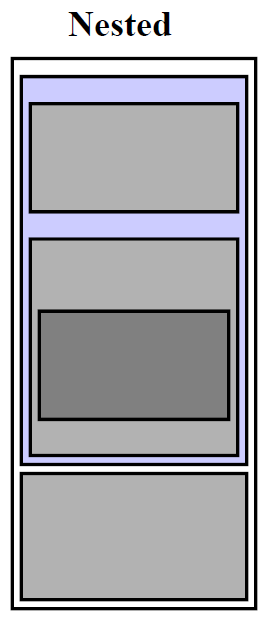
\includegraphics[scale=0.5]{rapport/5/figures/nested_block_structure}
		\end{center}	
		\caption{Illustration of the nested block structure}
		\label{nested_block_structure}
	\end{wrapfigure}


	%INCLUDE BIBLIOGRAPHY!!!	
	\begin{itemize}
	\item No identifier may be declared more than once within the same block (at the same level) %SPO
	\item For any applied occurrence there must be a corresponding occurrence, either within the same block or block which is higher up in the nesting. %SPO
	%INCLUDE BIBL...
	\end{itemize}
	
	
	Referring to figure \ref{nested_block_structure} which demonstrates the functioning of a nested block structure visually. Initially we consider how the nested block structure works in general and later an example of how the nested block structure works in the WAR programming language.
	
	One can have as many and as few blocks as needed, and every sub-block of an existing block, can use all the variables that have been declared in blocks over itself. 
	
	
	%Her kommer noget kode af vores egen for at beskrive hvordan nested block structure virker hos os.
		
\newpage
	
	
%Page 142 i Brown!! :D
		
\subsection{Type rules}
	These are the rules that checks the expressions form, and the type validity.
	
	\subsubsection*{Type rule of $<$}
		$E1 < E2$ is type correct and of type Boolean
		if $E1$ and $E2$ are type correct and of type Integer
	\subsubsection*{Type rule of $>$}
		$E1 > E2$ is type correct and of type Boolean
		if $E1$ and $E2$ are type correct and of type Integer
	\subsubsection*{Type rule of $==$}
		$E1 == E2$ is type correct and of type Boolean
		if $E1$ and $E2$ are type correct and of type Integer
	\subsubsection*{Type rule of $>=$}
		$E1 >= E2$ is type correct and of type Boolean
		if $E1$ and $E2$ are type correct and of type Integer
	\subsubsection*{Type rule of $<=$}
		$E1 <= E2$ is type correct and of type Boolean
		if $E1$ and $E2$ are type correct and of type Integer
	\subsubsection*{Type rule of $while$}
		$while(E){C}$ is type correct
		if $E$ is of type Boolean and $C$ is type correct
	\subsubsection*{Type rule of $if$}
		$if(E){C}$ is type correct
		if $E$ is of type Boolean and $C$ is type correct
	\subsubsection*{Type rule of $else if$}
		$else if(E){C}$ is type correct
		if $E$ is of type Boolean and $C$ is type correct
	\subsubsection*{Type rule of $else$}
		$else{C}$ is type correct
		if $C$ is type correct
	
	\subsubsection*{Type rule of $Position$}
		$Position(I1,I2)$ is type correct and of type Position
		if $I1$ and $I2$ are type correct and of type Integer	
	


%6. Implementation (Description of how we implemented it) - Visitor pattern (Page 320, Brown). - Why we chose C# (Maybe tombstone)

%This file only contains inputs!!!
\chapter{Game Description}
	\section{Syntax}
	The first step in writing our interpreter is to make a BNF of our language. BNF stands for {\it Backus Naur form} and is a way of
	structuring the language in a formal way, which will make it easy to implement. A BNF consists of a set of {\it production rules} and each
	production rule consists of: \\
	\begin{itemize}
		 \item Terminals: A {\it terminal } is a literal string that appears in the language in hand.
		 \item Non-terminal: A {\it non-terminal } consists of Non-terminals and Terminals, used for structuring the language.
	\end{itemize}
	
	\subsection*{Production Rule}
		A production rule has the form: \\
		$N ::= X$, \\
		where $X$ is a Non-terminal or a Terminal. \\
		
		The elements in a production rule can be identified by: \\
		Terminals are written in {\bf bold } and 
		Non-terminals are just written in plain text.
	\subsection*{Grouping of production rules}
		If we have two production rules on the form:\\
		$N ::= X$ \\
		$N ::= Y$ \\
		we are allowed to make a transformation: \\
		$N ::= X | Y$ \\
		Meaning $N$ is $X$ or $Y$ \\
	\subsection*{Example of a small BNF}
		\label{ex-bnf}
		\begin{center}
			\begin{tabular}{l l l}
				A		&	::=		&	 AB$ \mid $ B \\
				B		&	::=		&	{\bf b} $\mid$ {\bf n } $\mid$ {\bf f } \\
			\end{tabular}
		\end{center}
		This BNF would allow us to write programs like \\(We use $\rightarrow$ to show applying of a production rule): \\
		{\bf bnf}: A $\rightarrow$ AB $\rightarrow$ A{\bf f} $\rightarrow$ 
		AB{\bf f} $\rightarrow$A{\bf nf} $\rightarrow$ B{\bf nf}$\rightarrow${\bf bnf } \\
	
	\begin{comment}
	
	
	\subsubsection{Terminals}
	
	
		\begin{longtable}[l]{l}
			$\{$\\
			$\}$\\
			$>$\\
			$<$\\
			$($\\
			$)$\\
			$=$\\
			$+$\\
			$-$\\
			$*$\\
			$/$\\
			$\&$\\
			$|$\\
			$"$\\
			$,$\\
			$.$\\
			$;$\\
			$Attack$\\
			$AttackSpeed$\\
			$Behaviour$\\
			$Config$\\
			$Damage$\\
			$Distance$\\
			$else$\\
			$Grid$\\
			$Health$\
			$Height$\\
			$if$\\
			$Maxima$\\
			$Melee$\\
			$MoveAway$\\
			$Movement$\\
			$MoveTowards$\\
			$Position$\\
			$Range$\\
			$Ranged$\\
			$Regiment$\\
			$RegimentPosition$\\
			$Regiments$\\
			$Rules$\\
			$SearchForEnemies$\\
			$SearchForFriends$\\
			$Size$\\
			$Standards$\\
			$Team$\\
			$Teams$\\
			$Type$\\
			$While$\\
			$Width$\\
		\end{longtable}
%	\subsubsection{Nonterminals}
%		\begin{tabular}{l c}
%			Behaviour-Block   & Control-Structure   \\
%			Single-Command    & UnitStat 			\\
%			UnitStat-Name	  & Integer-Literal		\\
%			Comment			  & Team-File 			\\
%			Regiment-Block	  & Expression			\\
%			Operator		  & Config-File			\\
%			Grid-Block	      & Rules-Block 		\\
%			Maximums-Block	  & MaximumsStat		\\
%			MaximumsStat-Name & Standards-Block	 	\\
%			StandardsStat	  & StandardsStat-Name 	\\
%			Identifier		  & 					\\
%		\end{tabular}
\end{comment}
	\subsection{The BNF of the WAR Language}
		{\bf Notes}
		\begin{itemize}
			\item Digit represents one of the digits 0 through 9.
			\item Graphic represents a space or visible character.
			\item Letter represents one of the lower- or upper-case letters 'a','b',.....,or 'z'.
			\item eol represents an end-of-line 'character'.
		\end{itemize}
		\begin{center}
			\begin{longtable}{l l l}
				\endfirsthead
				\endhead
		Team-File					&	::=	&{\bf Team} Identifier Regiment-Block\\
		Identifier					&	::=	&Letter\\
									&$\mid$	&Identifier Digit\\
									&$\mid$	&Identifier Letter\\
		Block-Name					&	::=	&Identifier\\
		Regiment-Block				&	::=	&{\bf Regiment} Block-Name {\bf \{ } UnitStat Behaviour-Block \bf{\} }\\
									&$\mid$	&Regiment-Block {\bf Regiment} Block-Name\\
									&		&{\bf \{ } UnitStat Behaviour-Block \bf{\} }\\
		Behaviour-Block				&	::=	&{\bf Behaviour} Block-Name {\bf \{} Single-Command {\bf \}}  \\
									&$\mid$	& {\bf Behaviour} {\bf = } Block-Name{\bf ;} \\
		Regiment-Declaration			&	::=	&{\bf Regiment} Identifier {\bf =} Regiment-Search{\bf ;}\\
									&$\mid$	&{\bf Regiment} Identifier {\bf =} Block-Name{\bf ;}\\
		Regiment-Search				&	::=	&{\bf SearchForEnemies (}Parameters{\bf)}\\
									&$\mid$	&{\bf SearchForFriends(}Parameters{\bf)}\\
		RegimentStat				&	::=	&Identifier {\bf.} UnitStat-Type \\
		Parameters					&	::=	&UnitStat-Type Operator Integer-Literal\\
		 							&$\mid$	&Parameters{\bf ,} UnitStat-Type Operator Integer-Literal\\
		Single-Command				&	::=	&Control-Structure Single-Command \\
									&$\mid$	&Regiment-Declaration Single-Command\\
									&$\mid$	&UnitFunction Single-command\\
									&$\mid$	&Control-Structure\\
									&$\mid$	&UnitFunction\\
									&$\mid$	&Regiment-Declaration\\
		ElseIf-Structure			&	::=	&{\bf else if( } Expression{\bf )} {\bf \{ } Single-Command {\bf \} } ElseIf-Structure\\
									&$\mid$	&{\bf else if( } Expression{\bf )} {\bf \{ } Single-Command {\bf \} } \\
		Control-Structure			&	::=	&{\bf if( } Expression{\bf )} {\bf \{ } Single-Command {\bf \} }  \\
									&$\mid$	&{\bf if(} Expression {\bf )} {\bf \{ }Single-Command {\bf \}} \\
									&		&{\bf else } {\bf \{ }Single-Command {\bf \} } \\			
									&$\mid$	&{\bf if(} Expression {\bf )} {\bf \{ }Single-Command {\bf \}} \\
									&		&ElseIf-Structure {\bf else } {\bf \{ }Single-Command {\bf \} } \\
									&$\mid$	&{\bf if(} Expression {\bf )} {\bf \{ }Single-Command {\bf \}} ElseIf-Structure \\	
									&$\mid$	&{\bf while (} Expression {\bf )}{\bf \{ } Single-Command {\bf \}} \\
		Expression					&	::=	&Primary-Expression \\
									&$\mid$	&Expression Operator Primary-Expression \\
		Primary-Expression			&	::=	&(Expression)\\
									&$\mid$	&Integer-Literal \\
									&$\mid$	&UnitStat-Type \\
									&$\mid$	&RegimentStat \\
		Operator					&	::=	&$\boldsymbol {+}$\\
									&$\mid$	&$\boldsymbol {-}$\\
									&$\mid$	&$\boldsymbol {*}$\\
									&$\mid$	&$\boldsymbol {/}$\\
									&$\mid$	&$\boldsymbol {<}$\\
									&$\mid$	&$\boldsymbol {>}$\\
									&$\mid$	&$\boldsymbol {<=}$\\
									&$\mid$	&$\boldsymbol {>=}$\\
									&$\mid$	&$\boldsymbol {==}$\\
									&$\mid$	&$\boldsymbol {\&\&}$\\
									&$\mid$	&$\boldsymbol {\|}$\\
		UnitFunction				&	::=	&{\bf Attack(} Identifier {\bf );} \\
									&$\mid$	&{\bf MoveTowards(}Identifier {\bf );} \\
									&$\mid$	&{\bf MoveAway(} Identifier {\bf );} \\
		UnitStat					&	::=	&UnitStat-Declaration UnitStat \\
									&$\mid$	&UnitStat-Declaration \\
		UnitStat-Declaration		&	::=	&{\bf Size =} Integer-Literal{\bf ;} \\
									&$\mid$	&{\bf Type} = AttackType{\bf ;}\\
									&$\mid$	&{\bf  Range =} Integer-Literal{\bf;}\\
									&$\mid$	&{\bf Damage =} Integer-Literal{\bf ;}\\
									&$\mid$	&{\bf Movement = }Integer-Literal{\bf ;} \\				  
									&$\mid$	& {\bf RegimentPosition = Position(} Integer-Literal {\bf ,}\\
									&		& Integer-Literal {\bf );}\\
		UnitStat-Type				&	::=	&{\bf Size}\\
									&$\mid$	&{\bf Type}\\
									&$\mid$	&{\bf Range}\\
									&$\mid$	&{\bf Damage}\\
									&$\mid$	&{\bf Movement}\\
									&$\mid$	&{\bf AttackSpeed}\\
									&$\mid$	&{\bf Health}\\
									&$\mid$	&{\bf Distance}\\
		AttackType					&	::=	&{\bf Melee}\\
									&$\mid$	&{\bf Ranged}\\
		Integer-Literal				&	::=	&Digit\\
									&$\mid$	&Integer-Literal Digit\\
		Comment						&	::=	&{\bf //} Graphic-Literal eol\\
		Graphic-Literal				&	::=	&Graphic Graphic-Literal\\
									&$\mid$	&Graphic\\
		Config-File					&	::=	&{\bf Config} Grid-Block Rules-Block\\
		Grid-Block					&	::=	&{\bf Grid} Block-Name	 {\bf \{} GridStat \bf{\}}\\
		GridStat					&	::=	&GridStat-Declaration GridStat\\
									&$\mid$	&GridStat-Declaration \\
		GridStat-Declaration		&	::=	&{\bf Width = } Integer-Literal;\\
									&$\mid$	&{\bf Height = } Integer-Literal;\\
		Rules-Block					&	::=	&Standards-Block MaximumsBlock\\
		Maximums-Block				&	::=	&{\bf Maximums} {\bf \{} MaximumsStat {\bf \}} \\
		MaximumsStat				&	::=	&MaximumsStat-Declaration MaximumsStat\\
									&$\mid$	&MaximumsStat-Declaration\\
		MaximumsStat-Declaration	&	::=	&{\bf Regiments = } Integer-Literal{\bf ;}\\
									&$\mid$	&{\bf Teams = } Integer-Literal{\bf ;}\\
									&$\mid$	&{\bf Size = } Integer-Literal{\bf ;}\\
									&$\mid$	&{\bf Range = } Integer-Literal{\bf ;}\\
									&$\mid$	&{\bf Damage = } Integer-Literal{\bf ;}\\
									&$\mid$	&{\bf Movement = } Integer-Literal{\bf ;}\\
									&$\mid$	&{\bf AttackSpeed = } Integer-Literal{\bf ;}\\
									&$\mid$	&{\bf Health = } Integer-Literal{\bf ;}\\
		Standards-Block				&	::=	&{\bf Standards} {\bf \{ } UnitStat-Declaration Behaviour-Block\bf{\} }\\
			\end{longtable}
		\end{center}
		
		
	\subsection{EBNF}
		{\it EBNF} stands for {\it Extendend Backus Naur Form} and is, as the name refers to an extension of BNF.
		The EBNF allows us to use regular expressions to express production rules, which makes our rule set more compact and 
		easier to implement.
	
	\subsubsection*{Regular expressions}
		A regular expression is a convenient way of expressing strings. We use the following regular expressions: \\
		\begin{itemize}
			\item *(star): States that the terminal or non-terminal must be used 0 or more times.
			\item Parentheses: Used for grouping of non-terminals and terminals.
			\item $\epsilon$: Represents the empty string.
		\end{itemize}
		Please note that these regular expressions can only be used on the right side of the production rules. \\
		
		By using these regular expression we can \\
		transform the BNF example given in \ref{ex-bnf} to an EBNF: \\
		
		\begin{tabular}{l l l}
			B		&	::=		&	({\bf b} $\mid$ {\bf n } $\mid$ {\bf f })* \\
		\end{tabular}
		
		It's easy to see that the transformation made the rules more compact (we removed one the the production rules), but
		how do we transform a BNF to a EBNF in a systematic way? 
		This can be done by applying {\it left factorization }, {\it elimination of left recursion} and {\it substitution of non-terminals }.
		
		\subsubsection*{Left factorization}
			If we have a production rule on the form: \\
			\begin{tabular}{l l l}
				T		&	::=		&	AB$\mid$AC \\
			\end{tabular}
			
			We can do a left factorization: \\
			\begin{tabular}{l l l}
				T		&	::=		&	A(B$\mid$C) \\
			\end{tabular}
			
			This can be done because T will always start with an A and end with either a B or C.
			
		\subsubsection*{Elimination of left recursion}
			If we have a production rule on the form: \\
			\begin{tabular}{l l l}
				T		&	::=		&	A$\mid$TB \\
			\end{tabular}
			
			We can do an elimination of left recursion: \\
			\begin{tabular}{l l l}
				T		&	::=		&	A(B)* \\
			\end{tabular}
			
			To understand how we can do this look at the first production rule. To terminate the production rule we need 
			to put an A, so T will always consist of an A. When we are not selecting an A(, and terminating) we are only making B's, which is
			the same as B*.
		\subsubsection*{Substitution of non-terminals}
			If we have two production rules on the form: \\
			
			\begin{tabular}{l l l}
				T		&	::=		&	U $\mid$ AUC \\
				U		&	::=		&	{\bf ab} $\mid$ {\bf ba} \\
			\end{tabular} \\
			
			We can do a substitution of the non-terminal U for every production rule. This means that we 
			substitute any occurrence of U in a production rule with what is on the right hand side of U like this: \\
			
			\begin{tabular}{l l l}
				T		&	::=		&	({\bf ab} $\mid$ {\bf ba}) $\mid$ A ({\bf ab} $\mid$ {\bf ba})B \\
			\end{tabular}
	\subsection{The EBNF of the WAR Language}
		Left factorization, substituion of non-terminals 
		and elimination of left recursion was applied to transform the BNF to an EBNF. \\
		
		Substituion of non-terminals have removed the following non-terminals from the BNF: \\
		\begin{itemize}
			\item Else-If
			\item UnitStat
			\item Graphical-Literal
			\item GridStat
			\item MaximumsStat
		\end{itemize}
		
		\begin{center}
			\begin{longtable}{ l l l }
				\endfirsthead
				\endhead
		Team-File					&	::=	&{\bf Team} Identifier Regiment-Block*\\
		Identifier					&	::=	&Letter (Letter $\mid$ Digit)*\\
		Block-Name					&	::=	&Identifier\\
		Regiment-Block				&	::=	&{\bf Regiment} Block-Name {\bf \{ } \\
									&		&UnitStat-Declaration Behaviour-Block \bf{\} }\\
		Behaviour-Block				&	::=	&{\bf Behaviour}(Identifier{\bf \{ }Single-Command \bf{\} } $\mid$ {\bf $=$} Identifier)\\
		Regiment-Declaration		&	::=	&{\bf Regiment} Identifier {\bf =} Regiment-Search{\bf ;}\\
									&$\mid$	&{\bf Regiment} Identifier {\bf =} Block-Name{\bf ;}\\
		Regiment-Search				&	::=	&{\bf SearchForEnemies (} Parameters {\bf )}\\
									&$\mid$	&{\bf SearchForFriends(} Parameters {\bf )}\\
		RegimentStat				&	::=	&Identifier{\bf.}UnitStat-Type \\
		Parameters					&	::=	&UnitStat-Type Operator Integer-Literal\\
									&		&({\bf ,}UnitStat-Type Operator Integer-Literal)*\\
		Single-Command				&	::=	&(Control-Structure $\mid$ UnitFunction $\mid$ Regiment-Declaration)*\\
									&		&(Control-Structure $\mid$ UnitFunction $\mid$ Regiment-Declaration)\\		
		Control-Structure			&	::=	&if(Expression) \bf{\{}Single-Command \bf{\}}\\
									&		&(\bf{else if(}Expression\bf{)\{ }Single-Command\bf{ \}})* \\
									&		&($\epsilon$ $\mid$ else \bf{\{ }Single-Command \bf{\} }\\					   
									&$\mid$	&while(Expression)\bf{\{ } Single-Command \bf{\}}\\
		Expression					&	::=	&Primary-Expression (Operator Primary-Expression)*\\
		Primary-Expression			&	::=	&(Expression)\\
									&$\mid$	&Integer-Literal \\
									&$\mid$	&UnitStat-Type\\
									&$\mid$	&RegimentStat \\	
		Operator					&	::=	&$\boldsymbol {+}$\\
									&$\mid$	&$\boldsymbol {-}$\\
									&$\mid$	&$\boldsymbol {*}$\\
									&$\mid$	&$\boldsymbol {/}$\\
									&$\mid$	&$\boldsymbol {<}$\\
									&$\mid$	&$\boldsymbol {>}$\\
									&$\mid$	&$\boldsymbol {<=}$\\
									&$\mid$	&$\boldsymbol {>=}$\\
									&$\mid$	&$\boldsymbol {==}$\\
									&$\mid$	&$\boldsymbol {\&\&}$\\
									&$\mid$	&$\boldsymbol {\|}$\\
		UnitFunction				&	::=	&({\bf Attack} $\mid$ {\bf MoveTowards} $\mid${\bf MoveAway}){\bf (} Identifier {\bf );}\\
		UnitStat-Declaration		&	::=	&({\bf Size}$\mid${\bf Range}$\mid${\bf Damage} $\mid${\bf Movement}\\ 
									&		&$\mid$ {\bf AttackSpeed}$\mid${\bf Health}) ${\bf = }$ Integer-Literal{\bf ;} \\
									&$\mid$	&{\bf RegimentPosition =} \\
									&		&{\bf Position(}Integer-Literal{\bf ,}Integer-Literal{\bf );}\\
									&$\mid$	&{\bf Type} = AttackType{\bf ;}\\
		UnitStat-Type				&	::=	&({\bf Size}$\mid${\bf Range}$\mid${\bf Damage} $\mid$\\
									&		&{\bf Movement}$\mid$ {\bf AttackSpeed}$\mid${\bf Health}$\mid${\bf Distance})\\ 
		AttackType					&	::=	&{\bf Melee} $\mid$ {\bf Ranged} \\
		Integer-Literal				&	::=	&Digit Digit*\\
		Comment						&	::=	&{\bf //} Graphic* eol\\
		Config-File					&	::=	&{\bf Config} Grid-Block Rules-Block  		\\
		Grid-Block					&	::=	&{\bf Grid} Block-Name	 {\bf \{} GridStat-Declaration* \bf{\}} \\
		GridStat-Declaration		&	::=	&({\bf Width} $\mid$ {\bf Height})=  Integer-Literal{\bf ;} \\	
		Rules-Block					&	::=	&Standards-Block MaximumsBlock 				\\
		Maximums-Block				&	::=	&{\bf Maximums} {\bf \{} (MaximumsStat-Declaration)* {\bf \}}\\
		MaximumsStat-Declaration	&	::=	&({\bf Regiments }$\mid${\bf Teams}$\mid${\bf Size}$\mid$\\
									&		&{\bf Range}$\mid${\bf Damage}$\mid${\bf Movement}$\mid$\\
									&		&{\bf AttackSpeed}$\mid${\bf Health}) =  Integer-Literal{\bf ;}\\
		Standards-Block				&	::=	&{\bf Standards} {\bf \{ } UnitStat-Declaration* Behaviour-Block\bf{\} }		\\
			\end{longtable}
		\end{center}					     

	\section{Construction of the parser}
	In this section we will describe how one can construct a parser from a EBNF, but first we will describe how a parser is and how it works.
	
	\subsection{Parsing}
		The job of a parser is to check if a program is correct and 
		to determine the structure of the program, usually done by constructing tree structure.
		There are two ways of checking this {\it Bottom-up Parsing} and {\it Top-Down Parsing}.
		
		\subsubsection*{Bottom-up Parsing}
			This way of parsing takes simple structures and combining them to more complex structures.
			We show how this type of parsing works by applying Bottom-up parsing on this code written in : \\
			{\bf Maximums \{ Regiments = 5;\} }
			
			\begin{enumerate}
				\item Looks at 5 - Identifies it as an Integer-literal
				\item Looks at 5* -
			\end{enumerate}
			
	\section{Semantics}
\label{sec:conanal}
This section will define the scope and type rules of WAR.
	\subsection{Scope rules}
		A scope is a block of code, in WAR one is able to denote a new scope by using $\{$ to start the scope and $\}$.
		A scope placed inside another scope is called a {\it nested scope}. A {\it scope level} denotes how nested a given scope is,
		e.g. identifiers at scope level 0 is outside any scope, identifiers at scope level 1 is inside one scope etc.
		\begin{lstlisting}
		Scope
		{
			//Scope level 1
			identifier = 2
			Scope
			{
				//Scope level 2
				identifier = 2
			}
		}
		\end{lstlisting}
		
		Scope rules dictate the accessibility of identifiers from one scope to another.
	
	%These are the rules that defines how the identifiers must be read, and where to declare them - also known as identification.
	The WAR language has a nested block-structure which means we may have constants or variables can be defined in multiple scope levels. 
	Scope rules may be defined in levels, such that a declaration in the outermost block is at scope level 1, however, since the language has no declaration of variables, only constants, it works the same way. If you declare the $Size$ of a regiment at scope level 1, you can use $Size$ in all the higher scope levels. Declarations inside a block are referred to as being local in that block.

	The use of a nested block structure we follow some basic scope rules:
	\begin{wrapfigure}{r}{0.5\textwidth}
		\begin{center}
			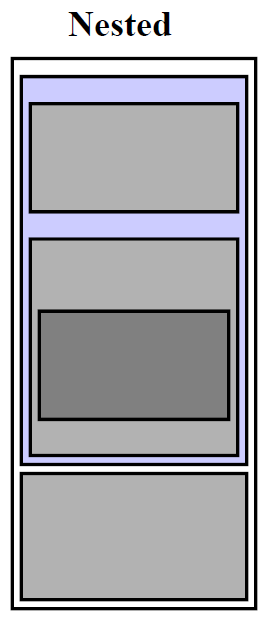
\includegraphics[scale=0.5]{rapport/5/figures/nested_block_structure}
		\end{center}	
		\caption{Illustration of the nested block structure}
		\label{nested_block_structure}
	\end{wrapfigure}


	%INCLUDE BIBLIOGRAPHY!!!	
	\begin{itemize}
	\item No identifier may be declared more than once within the same block (at the same level) %SPO
	\item For any applied occurrence there must be a corresponding occurrence, either within the same block or block which is higher up in the nesting. %SPO
	%INCLUDE BIBL...
	\end{itemize}
	
	
	Referring to figure \ref{nested_block_structure} which demonstrates the functioning of a nested block structure visually. Initially we consider how the nested block structure works in general and later an example of how the nested block structure works in the WAR programming language.
	
	One can have as many and as few blocks as needed, and every sub-block of an existing block, can use all the variables that have been declared in blocks over itself. 
	
	
	%Her kommer noget kode af vores egen for at beskrive hvordan nested block structure virker hos os.
		
\newpage
	
	
%Page 142 i Brown!! :D
		
\subsection{Type rules}
	These are the rules that checks the expressions form, and the type validity.
	
	\subsubsection*{Type rule of $<$}
		$E1 < E2$ is type correct and of type Boolean
		if $E1$ and $E2$ are type correct and of type Integer
	\subsubsection*{Type rule of $>$}
		$E1 > E2$ is type correct and of type Boolean
		if $E1$ and $E2$ are type correct and of type Integer
	\subsubsection*{Type rule of $==$}
		$E1 == E2$ is type correct and of type Boolean
		if $E1$ and $E2$ are type correct and of type Integer
	\subsubsection*{Type rule of $>=$}
		$E1 >= E2$ is type correct and of type Boolean
		if $E1$ and $E2$ are type correct and of type Integer
	\subsubsection*{Type rule of $<=$}
		$E1 <= E2$ is type correct and of type Boolean
		if $E1$ and $E2$ are type correct and of type Integer
	\subsubsection*{Type rule of $while$}
		$while(E){C}$ is type correct
		if $E$ is of type Boolean and $C$ is type correct
	\subsubsection*{Type rule of $if$}
		$if(E){C}$ is type correct
		if $E$ is of type Boolean and $C$ is type correct
	\subsubsection*{Type rule of $else if$}
		$else if(E){C}$ is type correct
		if $E$ is of type Boolean and $C$ is type correct
	\subsubsection*{Type rule of $else$}
		$else{C}$ is type correct
		if $C$ is type correct
	
	\subsubsection*{Type rule of $Position$}
		$Position(I1,I2)$ is type correct and of type Position
		if $I1$ and $I2$ are type correct and of type Integer	
	


%7. Usecases - (Example of the game (scripts, configs, screenshots etc.))

%This file only contains inputs!!!
\chapter{Game Description}
	\section{Syntax}
	The first step in writing our interpreter is to make a BNF of our language. BNF stands for {\it Backus Naur form} and is a way of
	structuring the language in a formal way, which will make it easy to implement. A BNF consists of a set of {\it production rules} and each
	production rule consists of: \\
	\begin{itemize}
		 \item Terminals: A {\it terminal } is a literal string that appears in the language in hand.
		 \item Non-terminal: A {\it non-terminal } consists of Non-terminals and Terminals, used for structuring the language.
	\end{itemize}
	
	\subsection*{Production Rule}
		A production rule has the form: \\
		$N ::= X$, \\
		where $X$ is a Non-terminal or a Terminal. \\
		
		The elements in a production rule can be identified by: \\
		Terminals are written in {\bf bold } and 
		Non-terminals are just written in plain text.
	\subsection*{Grouping of production rules}
		If we have two production rules on the form:\\
		$N ::= X$ \\
		$N ::= Y$ \\
		we are allowed to make a transformation: \\
		$N ::= X | Y$ \\
		Meaning $N$ is $X$ or $Y$ \\
	\subsection*{Example of a small BNF}
		\label{ex-bnf}
		\begin{center}
			\begin{tabular}{l l l}
				A		&	::=		&	 AB$ \mid $ B \\
				B		&	::=		&	{\bf b} $\mid$ {\bf n } $\mid$ {\bf f } \\
			\end{tabular}
		\end{center}
		This BNF would allow us to write programs like \\(We use $\rightarrow$ to show applying of a production rule): \\
		{\bf bnf}: A $\rightarrow$ AB $\rightarrow$ A{\bf f} $\rightarrow$ 
		AB{\bf f} $\rightarrow$A{\bf nf} $\rightarrow$ B{\bf nf}$\rightarrow${\bf bnf } \\
	
	\begin{comment}
	
	
	\subsubsection{Terminals}
	
	
		\begin{longtable}[l]{l}
			$\{$\\
			$\}$\\
			$>$\\
			$<$\\
			$($\\
			$)$\\
			$=$\\
			$+$\\
			$-$\\
			$*$\\
			$/$\\
			$\&$\\
			$|$\\
			$"$\\
			$,$\\
			$.$\\
			$;$\\
			$Attack$\\
			$AttackSpeed$\\
			$Behaviour$\\
			$Config$\\
			$Damage$\\
			$Distance$\\
			$else$\\
			$Grid$\\
			$Health$\
			$Height$\\
			$if$\\
			$Maxima$\\
			$Melee$\\
			$MoveAway$\\
			$Movement$\\
			$MoveTowards$\\
			$Position$\\
			$Range$\\
			$Ranged$\\
			$Regiment$\\
			$RegimentPosition$\\
			$Regiments$\\
			$Rules$\\
			$SearchForEnemies$\\
			$SearchForFriends$\\
			$Size$\\
			$Standards$\\
			$Team$\\
			$Teams$\\
			$Type$\\
			$While$\\
			$Width$\\
		\end{longtable}
%	\subsubsection{Nonterminals}
%		\begin{tabular}{l c}
%			Behaviour-Block   & Control-Structure   \\
%			Single-Command    & UnitStat 			\\
%			UnitStat-Name	  & Integer-Literal		\\
%			Comment			  & Team-File 			\\
%			Regiment-Block	  & Expression			\\
%			Operator		  & Config-File			\\
%			Grid-Block	      & Rules-Block 		\\
%			Maximums-Block	  & MaximumsStat		\\
%			MaximumsStat-Name & Standards-Block	 	\\
%			StandardsStat	  & StandardsStat-Name 	\\
%			Identifier		  & 					\\
%		\end{tabular}
\end{comment}
	\subsection{The BNF of the WAR Language}
		{\bf Notes}
		\begin{itemize}
			\item Digit represents one of the digits 0 through 9.
			\item Graphic represents a space or visible character.
			\item Letter represents one of the lower- or upper-case letters 'a','b',.....,or 'z'.
			\item eol represents an end-of-line 'character'.
		\end{itemize}
		\begin{center}
			\begin{longtable}{l l l}
				\endfirsthead
				\endhead
		Team-File					&	::=	&{\bf Team} Identifier Regiment-Block\\
		Identifier					&	::=	&Letter\\
									&$\mid$	&Identifier Digit\\
									&$\mid$	&Identifier Letter\\
		Block-Name					&	::=	&Identifier\\
		Regiment-Block				&	::=	&{\bf Regiment} Block-Name {\bf \{ } UnitStat Behaviour-Block \bf{\} }\\
									&$\mid$	&Regiment-Block {\bf Regiment} Block-Name\\
									&		&{\bf \{ } UnitStat Behaviour-Block \bf{\} }\\
		Behaviour-Block				&	::=	&{\bf Behaviour} Block-Name {\bf \{} Single-Command {\bf \}}  \\
									&$\mid$	& {\bf Behaviour} {\bf = } Block-Name{\bf ;} \\
		Regiment-Declaration			&	::=	&{\bf Regiment} Identifier {\bf =} Regiment-Search{\bf ;}\\
									&$\mid$	&{\bf Regiment} Identifier {\bf =} Block-Name{\bf ;}\\
		Regiment-Search				&	::=	&{\bf SearchForEnemies (}Parameters{\bf)}\\
									&$\mid$	&{\bf SearchForFriends(}Parameters{\bf)}\\
		RegimentStat				&	::=	&Identifier {\bf.} UnitStat-Type \\
		Parameters					&	::=	&UnitStat-Type Operator Integer-Literal\\
		 							&$\mid$	&Parameters{\bf ,} UnitStat-Type Operator Integer-Literal\\
		Single-Command				&	::=	&Control-Structure Single-Command \\
									&$\mid$	&Regiment-Declaration Single-Command\\
									&$\mid$	&UnitFunction Single-command\\
									&$\mid$	&Control-Structure\\
									&$\mid$	&UnitFunction\\
									&$\mid$	&Regiment-Declaration\\
		ElseIf-Structure			&	::=	&{\bf else if( } Expression{\bf )} {\bf \{ } Single-Command {\bf \} } ElseIf-Structure\\
									&$\mid$	&{\bf else if( } Expression{\bf )} {\bf \{ } Single-Command {\bf \} } \\
		Control-Structure			&	::=	&{\bf if( } Expression{\bf )} {\bf \{ } Single-Command {\bf \} }  \\
									&$\mid$	&{\bf if(} Expression {\bf )} {\bf \{ }Single-Command {\bf \}} \\
									&		&{\bf else } {\bf \{ }Single-Command {\bf \} } \\			
									&$\mid$	&{\bf if(} Expression {\bf )} {\bf \{ }Single-Command {\bf \}} \\
									&		&ElseIf-Structure {\bf else } {\bf \{ }Single-Command {\bf \} } \\
									&$\mid$	&{\bf if(} Expression {\bf )} {\bf \{ }Single-Command {\bf \}} ElseIf-Structure \\	
									&$\mid$	&{\bf while (} Expression {\bf )}{\bf \{ } Single-Command {\bf \}} \\
		Expression					&	::=	&Primary-Expression \\
									&$\mid$	&Expression Operator Primary-Expression \\
		Primary-Expression			&	::=	&(Expression)\\
									&$\mid$	&Integer-Literal \\
									&$\mid$	&UnitStat-Type \\
									&$\mid$	&RegimentStat \\
		Operator					&	::=	&$\boldsymbol {+}$\\
									&$\mid$	&$\boldsymbol {-}$\\
									&$\mid$	&$\boldsymbol {*}$\\
									&$\mid$	&$\boldsymbol {/}$\\
									&$\mid$	&$\boldsymbol {<}$\\
									&$\mid$	&$\boldsymbol {>}$\\
									&$\mid$	&$\boldsymbol {<=}$\\
									&$\mid$	&$\boldsymbol {>=}$\\
									&$\mid$	&$\boldsymbol {==}$\\
									&$\mid$	&$\boldsymbol {\&\&}$\\
									&$\mid$	&$\boldsymbol {\|}$\\
		UnitFunction				&	::=	&{\bf Attack(} Identifier {\bf );} \\
									&$\mid$	&{\bf MoveTowards(}Identifier {\bf );} \\
									&$\mid$	&{\bf MoveAway(} Identifier {\bf );} \\
		UnitStat					&	::=	&UnitStat-Declaration UnitStat \\
									&$\mid$	&UnitStat-Declaration \\
		UnitStat-Declaration		&	::=	&{\bf Size =} Integer-Literal{\bf ;} \\
									&$\mid$	&{\bf Type} = AttackType{\bf ;}\\
									&$\mid$	&{\bf  Range =} Integer-Literal{\bf;}\\
									&$\mid$	&{\bf Damage =} Integer-Literal{\bf ;}\\
									&$\mid$	&{\bf Movement = }Integer-Literal{\bf ;} \\				  
									&$\mid$	& {\bf RegimentPosition = Position(} Integer-Literal {\bf ,}\\
									&		& Integer-Literal {\bf );}\\
		UnitStat-Type				&	::=	&{\bf Size}\\
									&$\mid$	&{\bf Type}\\
									&$\mid$	&{\bf Range}\\
									&$\mid$	&{\bf Damage}\\
									&$\mid$	&{\bf Movement}\\
									&$\mid$	&{\bf AttackSpeed}\\
									&$\mid$	&{\bf Health}\\
									&$\mid$	&{\bf Distance}\\
		AttackType					&	::=	&{\bf Melee}\\
									&$\mid$	&{\bf Ranged}\\
		Integer-Literal				&	::=	&Digit\\
									&$\mid$	&Integer-Literal Digit\\
		Comment						&	::=	&{\bf //} Graphic-Literal eol\\
		Graphic-Literal				&	::=	&Graphic Graphic-Literal\\
									&$\mid$	&Graphic\\
		Config-File					&	::=	&{\bf Config} Grid-Block Rules-Block\\
		Grid-Block					&	::=	&{\bf Grid} Block-Name	 {\bf \{} GridStat \bf{\}}\\
		GridStat					&	::=	&GridStat-Declaration GridStat\\
									&$\mid$	&GridStat-Declaration \\
		GridStat-Declaration		&	::=	&{\bf Width = } Integer-Literal;\\
									&$\mid$	&{\bf Height = } Integer-Literal;\\
		Rules-Block					&	::=	&Standards-Block MaximumsBlock\\
		Maximums-Block				&	::=	&{\bf Maximums} {\bf \{} MaximumsStat {\bf \}} \\
		MaximumsStat				&	::=	&MaximumsStat-Declaration MaximumsStat\\
									&$\mid$	&MaximumsStat-Declaration\\
		MaximumsStat-Declaration	&	::=	&{\bf Regiments = } Integer-Literal{\bf ;}\\
									&$\mid$	&{\bf Teams = } Integer-Literal{\bf ;}\\
									&$\mid$	&{\bf Size = } Integer-Literal{\bf ;}\\
									&$\mid$	&{\bf Range = } Integer-Literal{\bf ;}\\
									&$\mid$	&{\bf Damage = } Integer-Literal{\bf ;}\\
									&$\mid$	&{\bf Movement = } Integer-Literal{\bf ;}\\
									&$\mid$	&{\bf AttackSpeed = } Integer-Literal{\bf ;}\\
									&$\mid$	&{\bf Health = } Integer-Literal{\bf ;}\\
		Standards-Block				&	::=	&{\bf Standards} {\bf \{ } UnitStat-Declaration Behaviour-Block\bf{\} }\\
			\end{longtable}
		\end{center}
		
		
	\subsection{EBNF}
		{\it EBNF} stands for {\it Extendend Backus Naur Form} and is, as the name refers to an extension of BNF.
		The EBNF allows us to use regular expressions to express production rules, which makes our rule set more compact and 
		easier to implement.
	
	\subsubsection*{Regular expressions}
		A regular expression is a convenient way of expressing strings. We use the following regular expressions: \\
		\begin{itemize}
			\item *(star): States that the terminal or non-terminal must be used 0 or more times.
			\item Parentheses: Used for grouping of non-terminals and terminals.
			\item $\epsilon$: Represents the empty string.
		\end{itemize}
		Please note that these regular expressions can only be used on the right side of the production rules. \\
		
		By using these regular expression we can \\
		transform the BNF example given in \ref{ex-bnf} to an EBNF: \\
		
		\begin{tabular}{l l l}
			B		&	::=		&	({\bf b} $\mid$ {\bf n } $\mid$ {\bf f })* \\
		\end{tabular}
		
		It's easy to see that the transformation made the rules more compact (we removed one the the production rules), but
		how do we transform a BNF to a EBNF in a systematic way? 
		This can be done by applying {\it left factorization }, {\it elimination of left recursion} and {\it substitution of non-terminals }.
		
		\subsubsection*{Left factorization}
			If we have a production rule on the form: \\
			\begin{tabular}{l l l}
				T		&	::=		&	AB$\mid$AC \\
			\end{tabular}
			
			We can do a left factorization: \\
			\begin{tabular}{l l l}
				T		&	::=		&	A(B$\mid$C) \\
			\end{tabular}
			
			This can be done because T will always start with an A and end with either a B or C.
			
		\subsubsection*{Elimination of left recursion}
			If we have a production rule on the form: \\
			\begin{tabular}{l l l}
				T		&	::=		&	A$\mid$TB \\
			\end{tabular}
			
			We can do an elimination of left recursion: \\
			\begin{tabular}{l l l}
				T		&	::=		&	A(B)* \\
			\end{tabular}
			
			To understand how we can do this look at the first production rule. To terminate the production rule we need 
			to put an A, so T will always consist of an A. When we are not selecting an A(, and terminating) we are only making B's, which is
			the same as B*.
		\subsubsection*{Substitution of non-terminals}
			If we have two production rules on the form: \\
			
			\begin{tabular}{l l l}
				T		&	::=		&	U $\mid$ AUC \\
				U		&	::=		&	{\bf ab} $\mid$ {\bf ba} \\
			\end{tabular} \\
			
			We can do a substitution of the non-terminal U for every production rule. This means that we 
			substitute any occurrence of U in a production rule with what is on the right hand side of U like this: \\
			
			\begin{tabular}{l l l}
				T		&	::=		&	({\bf ab} $\mid$ {\bf ba}) $\mid$ A ({\bf ab} $\mid$ {\bf ba})B \\
			\end{tabular}
	\subsection{The EBNF of the WAR Language}
		Left factorization, substituion of non-terminals 
		and elimination of left recursion was applied to transform the BNF to an EBNF. \\
		
		Substituion of non-terminals have removed the following non-terminals from the BNF: \\
		\begin{itemize}
			\item Else-If
			\item UnitStat
			\item Graphical-Literal
			\item GridStat
			\item MaximumsStat
		\end{itemize}
		
		\begin{center}
			\begin{longtable}{ l l l }
				\endfirsthead
				\endhead
		Team-File					&	::=	&{\bf Team} Identifier Regiment-Block*\\
		Identifier					&	::=	&Letter (Letter $\mid$ Digit)*\\
		Block-Name					&	::=	&Identifier\\
		Regiment-Block				&	::=	&{\bf Regiment} Block-Name {\bf \{ } \\
									&		&UnitStat-Declaration Behaviour-Block \bf{\} }\\
		Behaviour-Block				&	::=	&{\bf Behaviour}(Identifier{\bf \{ }Single-Command \bf{\} } $\mid$ {\bf $=$} Identifier)\\
		Regiment-Declaration		&	::=	&{\bf Regiment} Identifier {\bf =} Regiment-Search{\bf ;}\\
									&$\mid$	&{\bf Regiment} Identifier {\bf =} Block-Name{\bf ;}\\
		Regiment-Search				&	::=	&{\bf SearchForEnemies (} Parameters {\bf )}\\
									&$\mid$	&{\bf SearchForFriends(} Parameters {\bf )}\\
		RegimentStat				&	::=	&Identifier{\bf.}UnitStat-Type \\
		Parameters					&	::=	&UnitStat-Type Operator Integer-Literal\\
									&		&({\bf ,}UnitStat-Type Operator Integer-Literal)*\\
		Single-Command				&	::=	&(Control-Structure $\mid$ UnitFunction $\mid$ Regiment-Declaration)*\\
									&		&(Control-Structure $\mid$ UnitFunction $\mid$ Regiment-Declaration)\\		
		Control-Structure			&	::=	&if(Expression) \bf{\{}Single-Command \bf{\}}\\
									&		&(\bf{else if(}Expression\bf{)\{ }Single-Command\bf{ \}})* \\
									&		&($\epsilon$ $\mid$ else \bf{\{ }Single-Command \bf{\} }\\					   
									&$\mid$	&while(Expression)\bf{\{ } Single-Command \bf{\}}\\
		Expression					&	::=	&Primary-Expression (Operator Primary-Expression)*\\
		Primary-Expression			&	::=	&(Expression)\\
									&$\mid$	&Integer-Literal \\
									&$\mid$	&UnitStat-Type\\
									&$\mid$	&RegimentStat \\	
		Operator					&	::=	&$\boldsymbol {+}$\\
									&$\mid$	&$\boldsymbol {-}$\\
									&$\mid$	&$\boldsymbol {*}$\\
									&$\mid$	&$\boldsymbol {/}$\\
									&$\mid$	&$\boldsymbol {<}$\\
									&$\mid$	&$\boldsymbol {>}$\\
									&$\mid$	&$\boldsymbol {<=}$\\
									&$\mid$	&$\boldsymbol {>=}$\\
									&$\mid$	&$\boldsymbol {==}$\\
									&$\mid$	&$\boldsymbol {\&\&}$\\
									&$\mid$	&$\boldsymbol {\|}$\\
		UnitFunction				&	::=	&({\bf Attack} $\mid$ {\bf MoveTowards} $\mid${\bf MoveAway}){\bf (} Identifier {\bf );}\\
		UnitStat-Declaration		&	::=	&({\bf Size}$\mid${\bf Range}$\mid${\bf Damage} $\mid${\bf Movement}\\ 
									&		&$\mid$ {\bf AttackSpeed}$\mid${\bf Health}) ${\bf = }$ Integer-Literal{\bf ;} \\
									&$\mid$	&{\bf RegimentPosition =} \\
									&		&{\bf Position(}Integer-Literal{\bf ,}Integer-Literal{\bf );}\\
									&$\mid$	&{\bf Type} = AttackType{\bf ;}\\
		UnitStat-Type				&	::=	&({\bf Size}$\mid${\bf Range}$\mid${\bf Damage} $\mid$\\
									&		&{\bf Movement}$\mid$ {\bf AttackSpeed}$\mid${\bf Health}$\mid${\bf Distance})\\ 
		AttackType					&	::=	&{\bf Melee} $\mid$ {\bf Ranged} \\
		Integer-Literal				&	::=	&Digit Digit*\\
		Comment						&	::=	&{\bf //} Graphic* eol\\
		Config-File					&	::=	&{\bf Config} Grid-Block Rules-Block  		\\
		Grid-Block					&	::=	&{\bf Grid} Block-Name	 {\bf \{} GridStat-Declaration* \bf{\}} \\
		GridStat-Declaration		&	::=	&({\bf Width} $\mid$ {\bf Height})=  Integer-Literal{\bf ;} \\	
		Rules-Block					&	::=	&Standards-Block MaximumsBlock 				\\
		Maximums-Block				&	::=	&{\bf Maximums} {\bf \{} (MaximumsStat-Declaration)* {\bf \}}\\
		MaximumsStat-Declaration	&	::=	&({\bf Regiments }$\mid${\bf Teams}$\mid${\bf Size}$\mid$\\
									&		&{\bf Range}$\mid${\bf Damage}$\mid${\bf Movement}$\mid$\\
									&		&{\bf AttackSpeed}$\mid${\bf Health}) =  Integer-Literal{\bf ;}\\
		Standards-Block				&	::=	&{\bf Standards} {\bf \{ } UnitStat-Declaration* Behaviour-Block\bf{\} }		\\
			\end{longtable}
		\end{center}					     

	\section{Construction of the parser}
	In this section we will describe how one can construct a parser from a EBNF, but first we will describe how a parser is and how it works.
	
	\subsection{Parsing}
		The job of a parser is to check if a program is correct and 
		to determine the structure of the program, usually done by constructing tree structure.
		There are two ways of checking this {\it Bottom-up Parsing} and {\it Top-Down Parsing}.
		
		\subsubsection*{Bottom-up Parsing}
			This way of parsing takes simple structures and combining them to more complex structures.
			We show how this type of parsing works by applying Bottom-up parsing on this code written in : \\
			{\bf Maximums \{ Regiments = 5;\} }
			
			\begin{enumerate}
				\item Looks at 5 - Identifies it as an Integer-literal
				\item Looks at 5* -
			\end{enumerate}
			
	\section{Semantics}
\label{sec:conanal}
This section will define the scope and type rules of WAR.
	\subsection{Scope rules}
		A scope is a block of code, in WAR one is able to denote a new scope by using $\{$ to start the scope and $\}$.
		A scope placed inside another scope is called a {\it nested scope}. A {\it scope level} denotes how nested a given scope is,
		e.g. identifiers at scope level 0 is outside any scope, identifiers at scope level 1 is inside one scope etc.
		\begin{lstlisting}
		Scope
		{
			//Scope level 1
			identifier = 2
			Scope
			{
				//Scope level 2
				identifier = 2
			}
		}
		\end{lstlisting}
		
		Scope rules dictate the accessibility of identifiers from one scope to another.
	
	%These are the rules that defines how the identifiers must be read, and where to declare them - also known as identification.
	The WAR language has a nested block-structure which means we may have constants or variables can be defined in multiple scope levels. 
	Scope rules may be defined in levels, such that a declaration in the outermost block is at scope level 1, however, since the language has no declaration of variables, only constants, it works the same way. If you declare the $Size$ of a regiment at scope level 1, you can use $Size$ in all the higher scope levels. Declarations inside a block are referred to as being local in that block.

	The use of a nested block structure we follow some basic scope rules:
	\begin{wrapfigure}{r}{0.5\textwidth}
		\begin{center}
			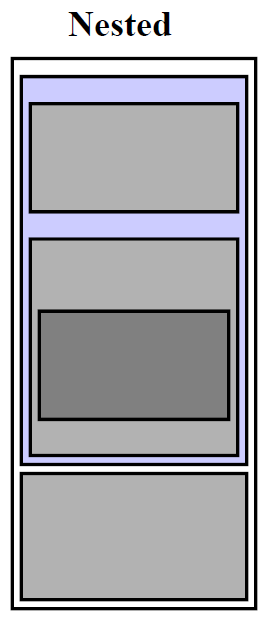
\includegraphics[scale=0.5]{rapport/5/figures/nested_block_structure}
		\end{center}	
		\caption{Illustration of the nested block structure}
		\label{nested_block_structure}
	\end{wrapfigure}


	%INCLUDE BIBLIOGRAPHY!!!	
	\begin{itemize}
	\item No identifier may be declared more than once within the same block (at the same level) %SPO
	\item For any applied occurrence there must be a corresponding occurrence, either within the same block or block which is higher up in the nesting. %SPO
	%INCLUDE BIBL...
	\end{itemize}
	
	
	Referring to figure \ref{nested_block_structure} which demonstrates the functioning of a nested block structure visually. Initially we consider how the nested block structure works in general and later an example of how the nested block structure works in the WAR programming language.
	
	One can have as many and as few blocks as needed, and every sub-block of an existing block, can use all the variables that have been declared in blocks over itself. 
	
	
	%Her kommer noget kode af vores egen for at beskrive hvordan nested block structure virker hos os.
		
\newpage
	
	
%Page 142 i Brown!! :D
		
\subsection{Type rules}
	These are the rules that checks the expressions form, and the type validity.
	
	\subsubsection*{Type rule of $<$}
		$E1 < E2$ is type correct and of type Boolean
		if $E1$ and $E2$ are type correct and of type Integer
	\subsubsection*{Type rule of $>$}
		$E1 > E2$ is type correct and of type Boolean
		if $E1$ and $E2$ are type correct and of type Integer
	\subsubsection*{Type rule of $==$}
		$E1 == E2$ is type correct and of type Boolean
		if $E1$ and $E2$ are type correct and of type Integer
	\subsubsection*{Type rule of $>=$}
		$E1 >= E2$ is type correct and of type Boolean
		if $E1$ and $E2$ are type correct and of type Integer
	\subsubsection*{Type rule of $<=$}
		$E1 <= E2$ is type correct and of type Boolean
		if $E1$ and $E2$ are type correct and of type Integer
	\subsubsection*{Type rule of $while$}
		$while(E){C}$ is type correct
		if $E$ is of type Boolean and $C$ is type correct
	\subsubsection*{Type rule of $if$}
		$if(E){C}$ is type correct
		if $E$ is of type Boolean and $C$ is type correct
	\subsubsection*{Type rule of $else if$}
		$else if(E){C}$ is type correct
		if $E$ is of type Boolean and $C$ is type correct
	\subsubsection*{Type rule of $else$}
		$else{C}$ is type correct
		if $C$ is type correct
	
	\subsubsection*{Type rule of $Position$}
		$Position(I1,I2)$ is type correct and of type Position
		if $I1$ and $I2$ are type correct and of type Integer	
	


%8. How to expand - (What we would have done if we had infinite time)

%This file only contains inputs!!!
\chapter{Game Description}
	\section{Syntax}
	The first step in writing our interpreter is to make a BNF of our language. BNF stands for {\it Backus Naur form} and is a way of
	structuring the language in a formal way, which will make it easy to implement. A BNF consists of a set of {\it production rules} and each
	production rule consists of: \\
	\begin{itemize}
		 \item Terminals: A {\it terminal } is a literal string that appears in the language in hand.
		 \item Non-terminal: A {\it non-terminal } consists of Non-terminals and Terminals, used for structuring the language.
	\end{itemize}
	
	\subsection*{Production Rule}
		A production rule has the form: \\
		$N ::= X$, \\
		where $X$ is a Non-terminal or a Terminal. \\
		
		The elements in a production rule can be identified by: \\
		Terminals are written in {\bf bold } and 
		Non-terminals are just written in plain text.
	\subsection*{Grouping of production rules}
		If we have two production rules on the form:\\
		$N ::= X$ \\
		$N ::= Y$ \\
		we are allowed to make a transformation: \\
		$N ::= X | Y$ \\
		Meaning $N$ is $X$ or $Y$ \\
	\subsection*{Example of a small BNF}
		\label{ex-bnf}
		\begin{center}
			\begin{tabular}{l l l}
				A		&	::=		&	 AB$ \mid $ B \\
				B		&	::=		&	{\bf b} $\mid$ {\bf n } $\mid$ {\bf f } \\
			\end{tabular}
		\end{center}
		This BNF would allow us to write programs like \\(We use $\rightarrow$ to show applying of a production rule): \\
		{\bf bnf}: A $\rightarrow$ AB $\rightarrow$ A{\bf f} $\rightarrow$ 
		AB{\bf f} $\rightarrow$A{\bf nf} $\rightarrow$ B{\bf nf}$\rightarrow${\bf bnf } \\
	
	\begin{comment}
	
	
	\subsubsection{Terminals}
	
	
		\begin{longtable}[l]{l}
			$\{$\\
			$\}$\\
			$>$\\
			$<$\\
			$($\\
			$)$\\
			$=$\\
			$+$\\
			$-$\\
			$*$\\
			$/$\\
			$\&$\\
			$|$\\
			$"$\\
			$,$\\
			$.$\\
			$;$\\
			$Attack$\\
			$AttackSpeed$\\
			$Behaviour$\\
			$Config$\\
			$Damage$\\
			$Distance$\\
			$else$\\
			$Grid$\\
			$Health$\
			$Height$\\
			$if$\\
			$Maxima$\\
			$Melee$\\
			$MoveAway$\\
			$Movement$\\
			$MoveTowards$\\
			$Position$\\
			$Range$\\
			$Ranged$\\
			$Regiment$\\
			$RegimentPosition$\\
			$Regiments$\\
			$Rules$\\
			$SearchForEnemies$\\
			$SearchForFriends$\\
			$Size$\\
			$Standards$\\
			$Team$\\
			$Teams$\\
			$Type$\\
			$While$\\
			$Width$\\
		\end{longtable}
%	\subsubsection{Nonterminals}
%		\begin{tabular}{l c}
%			Behaviour-Block   & Control-Structure   \\
%			Single-Command    & UnitStat 			\\
%			UnitStat-Name	  & Integer-Literal		\\
%			Comment			  & Team-File 			\\
%			Regiment-Block	  & Expression			\\
%			Operator		  & Config-File			\\
%			Grid-Block	      & Rules-Block 		\\
%			Maximums-Block	  & MaximumsStat		\\
%			MaximumsStat-Name & Standards-Block	 	\\
%			StandardsStat	  & StandardsStat-Name 	\\
%			Identifier		  & 					\\
%		\end{tabular}
\end{comment}
	\subsection{The BNF of the WAR Language}
		{\bf Notes}
		\begin{itemize}
			\item Digit represents one of the digits 0 through 9.
			\item Graphic represents a space or visible character.
			\item Letter represents one of the lower- or upper-case letters 'a','b',.....,or 'z'.
			\item eol represents an end-of-line 'character'.
		\end{itemize}
		\begin{center}
			\begin{longtable}{l l l}
				\endfirsthead
				\endhead
		Team-File					&	::=	&{\bf Team} Identifier Regiment-Block\\
		Identifier					&	::=	&Letter\\
									&$\mid$	&Identifier Digit\\
									&$\mid$	&Identifier Letter\\
		Block-Name					&	::=	&Identifier\\
		Regiment-Block				&	::=	&{\bf Regiment} Block-Name {\bf \{ } UnitStat Behaviour-Block \bf{\} }\\
									&$\mid$	&Regiment-Block {\bf Regiment} Block-Name\\
									&		&{\bf \{ } UnitStat Behaviour-Block \bf{\} }\\
		Behaviour-Block				&	::=	&{\bf Behaviour} Block-Name {\bf \{} Single-Command {\bf \}}  \\
									&$\mid$	& {\bf Behaviour} {\bf = } Block-Name{\bf ;} \\
		Regiment-Declaration			&	::=	&{\bf Regiment} Identifier {\bf =} Regiment-Search{\bf ;}\\
									&$\mid$	&{\bf Regiment} Identifier {\bf =} Block-Name{\bf ;}\\
		Regiment-Search				&	::=	&{\bf SearchForEnemies (}Parameters{\bf)}\\
									&$\mid$	&{\bf SearchForFriends(}Parameters{\bf)}\\
		RegimentStat				&	::=	&Identifier {\bf.} UnitStat-Type \\
		Parameters					&	::=	&UnitStat-Type Operator Integer-Literal\\
		 							&$\mid$	&Parameters{\bf ,} UnitStat-Type Operator Integer-Literal\\
		Single-Command				&	::=	&Control-Structure Single-Command \\
									&$\mid$	&Regiment-Declaration Single-Command\\
									&$\mid$	&UnitFunction Single-command\\
									&$\mid$	&Control-Structure\\
									&$\mid$	&UnitFunction\\
									&$\mid$	&Regiment-Declaration\\
		ElseIf-Structure			&	::=	&{\bf else if( } Expression{\bf )} {\bf \{ } Single-Command {\bf \} } ElseIf-Structure\\
									&$\mid$	&{\bf else if( } Expression{\bf )} {\bf \{ } Single-Command {\bf \} } \\
		Control-Structure			&	::=	&{\bf if( } Expression{\bf )} {\bf \{ } Single-Command {\bf \} }  \\
									&$\mid$	&{\bf if(} Expression {\bf )} {\bf \{ }Single-Command {\bf \}} \\
									&		&{\bf else } {\bf \{ }Single-Command {\bf \} } \\			
									&$\mid$	&{\bf if(} Expression {\bf )} {\bf \{ }Single-Command {\bf \}} \\
									&		&ElseIf-Structure {\bf else } {\bf \{ }Single-Command {\bf \} } \\
									&$\mid$	&{\bf if(} Expression {\bf )} {\bf \{ }Single-Command {\bf \}} ElseIf-Structure \\	
									&$\mid$	&{\bf while (} Expression {\bf )}{\bf \{ } Single-Command {\bf \}} \\
		Expression					&	::=	&Primary-Expression \\
									&$\mid$	&Expression Operator Primary-Expression \\
		Primary-Expression			&	::=	&(Expression)\\
									&$\mid$	&Integer-Literal \\
									&$\mid$	&UnitStat-Type \\
									&$\mid$	&RegimentStat \\
		Operator					&	::=	&$\boldsymbol {+}$\\
									&$\mid$	&$\boldsymbol {-}$\\
									&$\mid$	&$\boldsymbol {*}$\\
									&$\mid$	&$\boldsymbol {/}$\\
									&$\mid$	&$\boldsymbol {<}$\\
									&$\mid$	&$\boldsymbol {>}$\\
									&$\mid$	&$\boldsymbol {<=}$\\
									&$\mid$	&$\boldsymbol {>=}$\\
									&$\mid$	&$\boldsymbol {==}$\\
									&$\mid$	&$\boldsymbol {\&\&}$\\
									&$\mid$	&$\boldsymbol {\|}$\\
		UnitFunction				&	::=	&{\bf Attack(} Identifier {\bf );} \\
									&$\mid$	&{\bf MoveTowards(}Identifier {\bf );} \\
									&$\mid$	&{\bf MoveAway(} Identifier {\bf );} \\
		UnitStat					&	::=	&UnitStat-Declaration UnitStat \\
									&$\mid$	&UnitStat-Declaration \\
		UnitStat-Declaration		&	::=	&{\bf Size =} Integer-Literal{\bf ;} \\
									&$\mid$	&{\bf Type} = AttackType{\bf ;}\\
									&$\mid$	&{\bf  Range =} Integer-Literal{\bf;}\\
									&$\mid$	&{\bf Damage =} Integer-Literal{\bf ;}\\
									&$\mid$	&{\bf Movement = }Integer-Literal{\bf ;} \\				  
									&$\mid$	& {\bf RegimentPosition = Position(} Integer-Literal {\bf ,}\\
									&		& Integer-Literal {\bf );}\\
		UnitStat-Type				&	::=	&{\bf Size}\\
									&$\mid$	&{\bf Type}\\
									&$\mid$	&{\bf Range}\\
									&$\mid$	&{\bf Damage}\\
									&$\mid$	&{\bf Movement}\\
									&$\mid$	&{\bf AttackSpeed}\\
									&$\mid$	&{\bf Health}\\
									&$\mid$	&{\bf Distance}\\
		AttackType					&	::=	&{\bf Melee}\\
									&$\mid$	&{\bf Ranged}\\
		Integer-Literal				&	::=	&Digit\\
									&$\mid$	&Integer-Literal Digit\\
		Comment						&	::=	&{\bf //} Graphic-Literal eol\\
		Graphic-Literal				&	::=	&Graphic Graphic-Literal\\
									&$\mid$	&Graphic\\
		Config-File					&	::=	&{\bf Config} Grid-Block Rules-Block\\
		Grid-Block					&	::=	&{\bf Grid} Block-Name	 {\bf \{} GridStat \bf{\}}\\
		GridStat					&	::=	&GridStat-Declaration GridStat\\
									&$\mid$	&GridStat-Declaration \\
		GridStat-Declaration		&	::=	&{\bf Width = } Integer-Literal;\\
									&$\mid$	&{\bf Height = } Integer-Literal;\\
		Rules-Block					&	::=	&Standards-Block MaximumsBlock\\
		Maximums-Block				&	::=	&{\bf Maximums} {\bf \{} MaximumsStat {\bf \}} \\
		MaximumsStat				&	::=	&MaximumsStat-Declaration MaximumsStat\\
									&$\mid$	&MaximumsStat-Declaration\\
		MaximumsStat-Declaration	&	::=	&{\bf Regiments = } Integer-Literal{\bf ;}\\
									&$\mid$	&{\bf Teams = } Integer-Literal{\bf ;}\\
									&$\mid$	&{\bf Size = } Integer-Literal{\bf ;}\\
									&$\mid$	&{\bf Range = } Integer-Literal{\bf ;}\\
									&$\mid$	&{\bf Damage = } Integer-Literal{\bf ;}\\
									&$\mid$	&{\bf Movement = } Integer-Literal{\bf ;}\\
									&$\mid$	&{\bf AttackSpeed = } Integer-Literal{\bf ;}\\
									&$\mid$	&{\bf Health = } Integer-Literal{\bf ;}\\
		Standards-Block				&	::=	&{\bf Standards} {\bf \{ } UnitStat-Declaration Behaviour-Block\bf{\} }\\
			\end{longtable}
		\end{center}
		
		
	\subsection{EBNF}
		{\it EBNF} stands for {\it Extendend Backus Naur Form} and is, as the name refers to an extension of BNF.
		The EBNF allows us to use regular expressions to express production rules, which makes our rule set more compact and 
		easier to implement.
	
	\subsubsection*{Regular expressions}
		A regular expression is a convenient way of expressing strings. We use the following regular expressions: \\
		\begin{itemize}
			\item *(star): States that the terminal or non-terminal must be used 0 or more times.
			\item Parentheses: Used for grouping of non-terminals and terminals.
			\item $\epsilon$: Represents the empty string.
		\end{itemize}
		Please note that these regular expressions can only be used on the right side of the production rules. \\
		
		By using these regular expression we can \\
		transform the BNF example given in \ref{ex-bnf} to an EBNF: \\
		
		\begin{tabular}{l l l}
			B		&	::=		&	({\bf b} $\mid$ {\bf n } $\mid$ {\bf f })* \\
		\end{tabular}
		
		It's easy to see that the transformation made the rules more compact (we removed one the the production rules), but
		how do we transform a BNF to a EBNF in a systematic way? 
		This can be done by applying {\it left factorization }, {\it elimination of left recursion} and {\it substitution of non-terminals }.
		
		\subsubsection*{Left factorization}
			If we have a production rule on the form: \\
			\begin{tabular}{l l l}
				T		&	::=		&	AB$\mid$AC \\
			\end{tabular}
			
			We can do a left factorization: \\
			\begin{tabular}{l l l}
				T		&	::=		&	A(B$\mid$C) \\
			\end{tabular}
			
			This can be done because T will always start with an A and end with either a B or C.
			
		\subsubsection*{Elimination of left recursion}
			If we have a production rule on the form: \\
			\begin{tabular}{l l l}
				T		&	::=		&	A$\mid$TB \\
			\end{tabular}
			
			We can do an elimination of left recursion: \\
			\begin{tabular}{l l l}
				T		&	::=		&	A(B)* \\
			\end{tabular}
			
			To understand how we can do this look at the first production rule. To terminate the production rule we need 
			to put an A, so T will always consist of an A. When we are not selecting an A(, and terminating) we are only making B's, which is
			the same as B*.
		\subsubsection*{Substitution of non-terminals}
			If we have two production rules on the form: \\
			
			\begin{tabular}{l l l}
				T		&	::=		&	U $\mid$ AUC \\
				U		&	::=		&	{\bf ab} $\mid$ {\bf ba} \\
			\end{tabular} \\
			
			We can do a substitution of the non-terminal U for every production rule. This means that we 
			substitute any occurrence of U in a production rule with what is on the right hand side of U like this: \\
			
			\begin{tabular}{l l l}
				T		&	::=		&	({\bf ab} $\mid$ {\bf ba}) $\mid$ A ({\bf ab} $\mid$ {\bf ba})B \\
			\end{tabular}
	\subsection{The EBNF of the WAR Language}
		Left factorization, substituion of non-terminals 
		and elimination of left recursion was applied to transform the BNF to an EBNF. \\
		
		Substituion of non-terminals have removed the following non-terminals from the BNF: \\
		\begin{itemize}
			\item Else-If
			\item UnitStat
			\item Graphical-Literal
			\item GridStat
			\item MaximumsStat
		\end{itemize}
		
		\begin{center}
			\begin{longtable}{ l l l }
				\endfirsthead
				\endhead
		Team-File					&	::=	&{\bf Team} Identifier Regiment-Block*\\
		Identifier					&	::=	&Letter (Letter $\mid$ Digit)*\\
		Block-Name					&	::=	&Identifier\\
		Regiment-Block				&	::=	&{\bf Regiment} Block-Name {\bf \{ } \\
									&		&UnitStat-Declaration Behaviour-Block \bf{\} }\\
		Behaviour-Block				&	::=	&{\bf Behaviour}(Identifier{\bf \{ }Single-Command \bf{\} } $\mid$ {\bf $=$} Identifier)\\
		Regiment-Declaration		&	::=	&{\bf Regiment} Identifier {\bf =} Regiment-Search{\bf ;}\\
									&$\mid$	&{\bf Regiment} Identifier {\bf =} Block-Name{\bf ;}\\
		Regiment-Search				&	::=	&{\bf SearchForEnemies (} Parameters {\bf )}\\
									&$\mid$	&{\bf SearchForFriends(} Parameters {\bf )}\\
		RegimentStat				&	::=	&Identifier{\bf.}UnitStat-Type \\
		Parameters					&	::=	&UnitStat-Type Operator Integer-Literal\\
									&		&({\bf ,}UnitStat-Type Operator Integer-Literal)*\\
		Single-Command				&	::=	&(Control-Structure $\mid$ UnitFunction $\mid$ Regiment-Declaration)*\\
									&		&(Control-Structure $\mid$ UnitFunction $\mid$ Regiment-Declaration)\\		
		Control-Structure			&	::=	&if(Expression) \bf{\{}Single-Command \bf{\}}\\
									&		&(\bf{else if(}Expression\bf{)\{ }Single-Command\bf{ \}})* \\
									&		&($\epsilon$ $\mid$ else \bf{\{ }Single-Command \bf{\} }\\					   
									&$\mid$	&while(Expression)\bf{\{ } Single-Command \bf{\}}\\
		Expression					&	::=	&Primary-Expression (Operator Primary-Expression)*\\
		Primary-Expression			&	::=	&(Expression)\\
									&$\mid$	&Integer-Literal \\
									&$\mid$	&UnitStat-Type\\
									&$\mid$	&RegimentStat \\	
		Operator					&	::=	&$\boldsymbol {+}$\\
									&$\mid$	&$\boldsymbol {-}$\\
									&$\mid$	&$\boldsymbol {*}$\\
									&$\mid$	&$\boldsymbol {/}$\\
									&$\mid$	&$\boldsymbol {<}$\\
									&$\mid$	&$\boldsymbol {>}$\\
									&$\mid$	&$\boldsymbol {<=}$\\
									&$\mid$	&$\boldsymbol {>=}$\\
									&$\mid$	&$\boldsymbol {==}$\\
									&$\mid$	&$\boldsymbol {\&\&}$\\
									&$\mid$	&$\boldsymbol {\|}$\\
		UnitFunction				&	::=	&({\bf Attack} $\mid$ {\bf MoveTowards} $\mid${\bf MoveAway}){\bf (} Identifier {\bf );}\\
		UnitStat-Declaration		&	::=	&({\bf Size}$\mid${\bf Range}$\mid${\bf Damage} $\mid${\bf Movement}\\ 
									&		&$\mid$ {\bf AttackSpeed}$\mid${\bf Health}) ${\bf = }$ Integer-Literal{\bf ;} \\
									&$\mid$	&{\bf RegimentPosition =} \\
									&		&{\bf Position(}Integer-Literal{\bf ,}Integer-Literal{\bf );}\\
									&$\mid$	&{\bf Type} = AttackType{\bf ;}\\
		UnitStat-Type				&	::=	&({\bf Size}$\mid${\bf Range}$\mid${\bf Damage} $\mid$\\
									&		&{\bf Movement}$\mid$ {\bf AttackSpeed}$\mid${\bf Health}$\mid${\bf Distance})\\ 
		AttackType					&	::=	&{\bf Melee} $\mid$ {\bf Ranged} \\
		Integer-Literal				&	::=	&Digit Digit*\\
		Comment						&	::=	&{\bf //} Graphic* eol\\
		Config-File					&	::=	&{\bf Config} Grid-Block Rules-Block  		\\
		Grid-Block					&	::=	&{\bf Grid} Block-Name	 {\bf \{} GridStat-Declaration* \bf{\}} \\
		GridStat-Declaration		&	::=	&({\bf Width} $\mid$ {\bf Height})=  Integer-Literal{\bf ;} \\	
		Rules-Block					&	::=	&Standards-Block MaximumsBlock 				\\
		Maximums-Block				&	::=	&{\bf Maximums} {\bf \{} (MaximumsStat-Declaration)* {\bf \}}\\
		MaximumsStat-Declaration	&	::=	&({\bf Regiments }$\mid${\bf Teams}$\mid${\bf Size}$\mid$\\
									&		&{\bf Range}$\mid${\bf Damage}$\mid${\bf Movement}$\mid$\\
									&		&{\bf AttackSpeed}$\mid${\bf Health}) =  Integer-Literal{\bf ;}\\
		Standards-Block				&	::=	&{\bf Standards} {\bf \{ } UnitStat-Declaration* Behaviour-Block\bf{\} }		\\
			\end{longtable}
		\end{center}					     

	\section{Construction of the parser}
	In this section we will describe how one can construct a parser from a EBNF, but first we will describe how a parser is and how it works.
	
	\subsection{Parsing}
		The job of a parser is to check if a program is correct and 
		to determine the structure of the program, usually done by constructing tree structure.
		There are two ways of checking this {\it Bottom-up Parsing} and {\it Top-Down Parsing}.
		
		\subsubsection*{Bottom-up Parsing}
			This way of parsing takes simple structures and combining them to more complex structures.
			We show how this type of parsing works by applying Bottom-up parsing on this code written in : \\
			{\bf Maximums \{ Regiments = 5;\} }
			
			\begin{enumerate}
				\item Looks at 5 - Identifies it as an Integer-literal
				\item Looks at 5* -
			\end{enumerate}
			
	\section{Semantics}
\label{sec:conanal}
This section will define the scope and type rules of WAR.
	\subsection{Scope rules}
		A scope is a block of code, in WAR one is able to denote a new scope by using $\{$ to start the scope and $\}$.
		A scope placed inside another scope is called a {\it nested scope}. A {\it scope level} denotes how nested a given scope is,
		e.g. identifiers at scope level 0 is outside any scope, identifiers at scope level 1 is inside one scope etc.
		\begin{lstlisting}
		Scope
		{
			//Scope level 1
			identifier = 2
			Scope
			{
				//Scope level 2
				identifier = 2
			}
		}
		\end{lstlisting}
		
		Scope rules dictate the accessibility of identifiers from one scope to another.
	
	%These are the rules that defines how the identifiers must be read, and where to declare them - also known as identification.
	The WAR language has a nested block-structure which means we may have constants or variables can be defined in multiple scope levels. 
	Scope rules may be defined in levels, such that a declaration in the outermost block is at scope level 1, however, since the language has no declaration of variables, only constants, it works the same way. If you declare the $Size$ of a regiment at scope level 1, you can use $Size$ in all the higher scope levels. Declarations inside a block are referred to as being local in that block.

	The use of a nested block structure we follow some basic scope rules:
	\begin{wrapfigure}{r}{0.5\textwidth}
		\begin{center}
			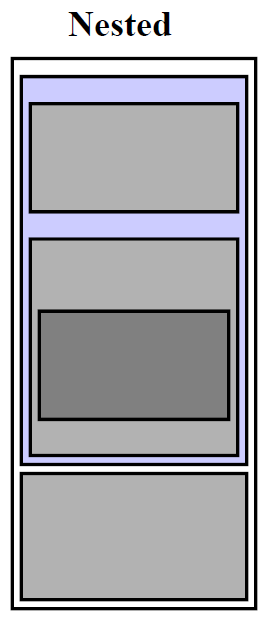
\includegraphics[scale=0.5]{rapport/5/figures/nested_block_structure}
		\end{center}	
		\caption{Illustration of the nested block structure}
		\label{nested_block_structure}
	\end{wrapfigure}


	%INCLUDE BIBLIOGRAPHY!!!	
	\begin{itemize}
	\item No identifier may be declared more than once within the same block (at the same level) %SPO
	\item For any applied occurrence there must be a corresponding occurrence, either within the same block or block which is higher up in the nesting. %SPO
	%INCLUDE BIBL...
	\end{itemize}
	
	
	Referring to figure \ref{nested_block_structure} which demonstrates the functioning of a nested block structure visually. Initially we consider how the nested block structure works in general and later an example of how the nested block structure works in the WAR programming language.
	
	One can have as many and as few blocks as needed, and every sub-block of an existing block, can use all the variables that have been declared in blocks over itself. 
	
	
	%Her kommer noget kode af vores egen for at beskrive hvordan nested block structure virker hos os.
		
\newpage
	
	
%Page 142 i Brown!! :D
		
\subsection{Type rules}
	These are the rules that checks the expressions form, and the type validity.
	
	\subsubsection*{Type rule of $<$}
		$E1 < E2$ is type correct and of type Boolean
		if $E1$ and $E2$ are type correct and of type Integer
	\subsubsection*{Type rule of $>$}
		$E1 > E2$ is type correct and of type Boolean
		if $E1$ and $E2$ are type correct and of type Integer
	\subsubsection*{Type rule of $==$}
		$E1 == E2$ is type correct and of type Boolean
		if $E1$ and $E2$ are type correct and of type Integer
	\subsubsection*{Type rule of $>=$}
		$E1 >= E2$ is type correct and of type Boolean
		if $E1$ and $E2$ are type correct and of type Integer
	\subsubsection*{Type rule of $<=$}
		$E1 <= E2$ is type correct and of type Boolean
		if $E1$ and $E2$ are type correct and of type Integer
	\subsubsection*{Type rule of $while$}
		$while(E){C}$ is type correct
		if $E$ is of type Boolean and $C$ is type correct
	\subsubsection*{Type rule of $if$}
		$if(E){C}$ is type correct
		if $E$ is of type Boolean and $C$ is type correct
	\subsubsection*{Type rule of $else if$}
		$else if(E){C}$ is type correct
		if $E$ is of type Boolean and $C$ is type correct
	\subsubsection*{Type rule of $else$}
		$else{C}$ is type correct
		if $C$ is type correct
	
	\subsubsection*{Type rule of $Position$}
		$Position(I1,I2)$ is type correct and of type Position
		if $I1$ and $I2$ are type correct and of type Integer	
	


%9. Conclusion - Dicussion

%This file only contains inputs!!!
\chapter{Game Description}
	\section{Syntax}
	The first step in writing our interpreter is to make a BNF of our language. BNF stands for {\it Backus Naur form} and is a way of
	structuring the language in a formal way, which will make it easy to implement. A BNF consists of a set of {\it production rules} and each
	production rule consists of: \\
	\begin{itemize}
		 \item Terminals: A {\it terminal } is a literal string that appears in the language in hand.
		 \item Non-terminal: A {\it non-terminal } consists of Non-terminals and Terminals, used for structuring the language.
	\end{itemize}
	
	\subsection*{Production Rule}
		A production rule has the form: \\
		$N ::= X$, \\
		where $X$ is a Non-terminal or a Terminal. \\
		
		The elements in a production rule can be identified by: \\
		Terminals are written in {\bf bold } and 
		Non-terminals are just written in plain text.
	\subsection*{Grouping of production rules}
		If we have two production rules on the form:\\
		$N ::= X$ \\
		$N ::= Y$ \\
		we are allowed to make a transformation: \\
		$N ::= X | Y$ \\
		Meaning $N$ is $X$ or $Y$ \\
	\subsection*{Example of a small BNF}
		\label{ex-bnf}
		\begin{center}
			\begin{tabular}{l l l}
				A		&	::=		&	 AB$ \mid $ B \\
				B		&	::=		&	{\bf b} $\mid$ {\bf n } $\mid$ {\bf f } \\
			\end{tabular}
		\end{center}
		This BNF would allow us to write programs like \\(We use $\rightarrow$ to show applying of a production rule): \\
		{\bf bnf}: A $\rightarrow$ AB $\rightarrow$ A{\bf f} $\rightarrow$ 
		AB{\bf f} $\rightarrow$A{\bf nf} $\rightarrow$ B{\bf nf}$\rightarrow${\bf bnf } \\
	
	\begin{comment}
	
	
	\subsubsection{Terminals}
	
	
		\begin{longtable}[l]{l}
			$\{$\\
			$\}$\\
			$>$\\
			$<$\\
			$($\\
			$)$\\
			$=$\\
			$+$\\
			$-$\\
			$*$\\
			$/$\\
			$\&$\\
			$|$\\
			$"$\\
			$,$\\
			$.$\\
			$;$\\
			$Attack$\\
			$AttackSpeed$\\
			$Behaviour$\\
			$Config$\\
			$Damage$\\
			$Distance$\\
			$else$\\
			$Grid$\\
			$Health$\
			$Height$\\
			$if$\\
			$Maxima$\\
			$Melee$\\
			$MoveAway$\\
			$Movement$\\
			$MoveTowards$\\
			$Position$\\
			$Range$\\
			$Ranged$\\
			$Regiment$\\
			$RegimentPosition$\\
			$Regiments$\\
			$Rules$\\
			$SearchForEnemies$\\
			$SearchForFriends$\\
			$Size$\\
			$Standards$\\
			$Team$\\
			$Teams$\\
			$Type$\\
			$While$\\
			$Width$\\
		\end{longtable}
%	\subsubsection{Nonterminals}
%		\begin{tabular}{l c}
%			Behaviour-Block   & Control-Structure   \\
%			Single-Command    & UnitStat 			\\
%			UnitStat-Name	  & Integer-Literal		\\
%			Comment			  & Team-File 			\\
%			Regiment-Block	  & Expression			\\
%			Operator		  & Config-File			\\
%			Grid-Block	      & Rules-Block 		\\
%			Maximums-Block	  & MaximumsStat		\\
%			MaximumsStat-Name & Standards-Block	 	\\
%			StandardsStat	  & StandardsStat-Name 	\\
%			Identifier		  & 					\\
%		\end{tabular}
\end{comment}
	\subsection{The BNF of the WAR Language}
		{\bf Notes}
		\begin{itemize}
			\item Digit represents one of the digits 0 through 9.
			\item Graphic represents a space or visible character.
			\item Letter represents one of the lower- or upper-case letters 'a','b',.....,or 'z'.
			\item eol represents an end-of-line 'character'.
		\end{itemize}
		\begin{center}
			\begin{longtable}{l l l}
				\endfirsthead
				\endhead
		Team-File					&	::=	&{\bf Team} Identifier Regiment-Block\\
		Identifier					&	::=	&Letter\\
									&$\mid$	&Identifier Digit\\
									&$\mid$	&Identifier Letter\\
		Block-Name					&	::=	&Identifier\\
		Regiment-Block				&	::=	&{\bf Regiment} Block-Name {\bf \{ } UnitStat Behaviour-Block \bf{\} }\\
									&$\mid$	&Regiment-Block {\bf Regiment} Block-Name\\
									&		&{\bf \{ } UnitStat Behaviour-Block \bf{\} }\\
		Behaviour-Block				&	::=	&{\bf Behaviour} Block-Name {\bf \{} Single-Command {\bf \}}  \\
									&$\mid$	& {\bf Behaviour} {\bf = } Block-Name{\bf ;} \\
		Regiment-Declaration			&	::=	&{\bf Regiment} Identifier {\bf =} Regiment-Search{\bf ;}\\
									&$\mid$	&{\bf Regiment} Identifier {\bf =} Block-Name{\bf ;}\\
		Regiment-Search				&	::=	&{\bf SearchForEnemies (}Parameters{\bf)}\\
									&$\mid$	&{\bf SearchForFriends(}Parameters{\bf)}\\
		RegimentStat				&	::=	&Identifier {\bf.} UnitStat-Type \\
		Parameters					&	::=	&UnitStat-Type Operator Integer-Literal\\
		 							&$\mid$	&Parameters{\bf ,} UnitStat-Type Operator Integer-Literal\\
		Single-Command				&	::=	&Control-Structure Single-Command \\
									&$\mid$	&Regiment-Declaration Single-Command\\
									&$\mid$	&UnitFunction Single-command\\
									&$\mid$	&Control-Structure\\
									&$\mid$	&UnitFunction\\
									&$\mid$	&Regiment-Declaration\\
		ElseIf-Structure			&	::=	&{\bf else if( } Expression{\bf )} {\bf \{ } Single-Command {\bf \} } ElseIf-Structure\\
									&$\mid$	&{\bf else if( } Expression{\bf )} {\bf \{ } Single-Command {\bf \} } \\
		Control-Structure			&	::=	&{\bf if( } Expression{\bf )} {\bf \{ } Single-Command {\bf \} }  \\
									&$\mid$	&{\bf if(} Expression {\bf )} {\bf \{ }Single-Command {\bf \}} \\
									&		&{\bf else } {\bf \{ }Single-Command {\bf \} } \\			
									&$\mid$	&{\bf if(} Expression {\bf )} {\bf \{ }Single-Command {\bf \}} \\
									&		&ElseIf-Structure {\bf else } {\bf \{ }Single-Command {\bf \} } \\
									&$\mid$	&{\bf if(} Expression {\bf )} {\bf \{ }Single-Command {\bf \}} ElseIf-Structure \\	
									&$\mid$	&{\bf while (} Expression {\bf )}{\bf \{ } Single-Command {\bf \}} \\
		Expression					&	::=	&Primary-Expression \\
									&$\mid$	&Expression Operator Primary-Expression \\
		Primary-Expression			&	::=	&(Expression)\\
									&$\mid$	&Integer-Literal \\
									&$\mid$	&UnitStat-Type \\
									&$\mid$	&RegimentStat \\
		Operator					&	::=	&$\boldsymbol {+}$\\
									&$\mid$	&$\boldsymbol {-}$\\
									&$\mid$	&$\boldsymbol {*}$\\
									&$\mid$	&$\boldsymbol {/}$\\
									&$\mid$	&$\boldsymbol {<}$\\
									&$\mid$	&$\boldsymbol {>}$\\
									&$\mid$	&$\boldsymbol {<=}$\\
									&$\mid$	&$\boldsymbol {>=}$\\
									&$\mid$	&$\boldsymbol {==}$\\
									&$\mid$	&$\boldsymbol {\&\&}$\\
									&$\mid$	&$\boldsymbol {\|}$\\
		UnitFunction				&	::=	&{\bf Attack(} Identifier {\bf );} \\
									&$\mid$	&{\bf MoveTowards(}Identifier {\bf );} \\
									&$\mid$	&{\bf MoveAway(} Identifier {\bf );} \\
		UnitStat					&	::=	&UnitStat-Declaration UnitStat \\
									&$\mid$	&UnitStat-Declaration \\
		UnitStat-Declaration		&	::=	&{\bf Size =} Integer-Literal{\bf ;} \\
									&$\mid$	&{\bf Type} = AttackType{\bf ;}\\
									&$\mid$	&{\bf  Range =} Integer-Literal{\bf;}\\
									&$\mid$	&{\bf Damage =} Integer-Literal{\bf ;}\\
									&$\mid$	&{\bf Movement = }Integer-Literal{\bf ;} \\				  
									&$\mid$	& {\bf RegimentPosition = Position(} Integer-Literal {\bf ,}\\
									&		& Integer-Literal {\bf );}\\
		UnitStat-Type				&	::=	&{\bf Size}\\
									&$\mid$	&{\bf Type}\\
									&$\mid$	&{\bf Range}\\
									&$\mid$	&{\bf Damage}\\
									&$\mid$	&{\bf Movement}\\
									&$\mid$	&{\bf AttackSpeed}\\
									&$\mid$	&{\bf Health}\\
									&$\mid$	&{\bf Distance}\\
		AttackType					&	::=	&{\bf Melee}\\
									&$\mid$	&{\bf Ranged}\\
		Integer-Literal				&	::=	&Digit\\
									&$\mid$	&Integer-Literal Digit\\
		Comment						&	::=	&{\bf //} Graphic-Literal eol\\
		Graphic-Literal				&	::=	&Graphic Graphic-Literal\\
									&$\mid$	&Graphic\\
		Config-File					&	::=	&{\bf Config} Grid-Block Rules-Block\\
		Grid-Block					&	::=	&{\bf Grid} Block-Name	 {\bf \{} GridStat \bf{\}}\\
		GridStat					&	::=	&GridStat-Declaration GridStat\\
									&$\mid$	&GridStat-Declaration \\
		GridStat-Declaration		&	::=	&{\bf Width = } Integer-Literal;\\
									&$\mid$	&{\bf Height = } Integer-Literal;\\
		Rules-Block					&	::=	&Standards-Block MaximumsBlock\\
		Maximums-Block				&	::=	&{\bf Maximums} {\bf \{} MaximumsStat {\bf \}} \\
		MaximumsStat				&	::=	&MaximumsStat-Declaration MaximumsStat\\
									&$\mid$	&MaximumsStat-Declaration\\
		MaximumsStat-Declaration	&	::=	&{\bf Regiments = } Integer-Literal{\bf ;}\\
									&$\mid$	&{\bf Teams = } Integer-Literal{\bf ;}\\
									&$\mid$	&{\bf Size = } Integer-Literal{\bf ;}\\
									&$\mid$	&{\bf Range = } Integer-Literal{\bf ;}\\
									&$\mid$	&{\bf Damage = } Integer-Literal{\bf ;}\\
									&$\mid$	&{\bf Movement = } Integer-Literal{\bf ;}\\
									&$\mid$	&{\bf AttackSpeed = } Integer-Literal{\bf ;}\\
									&$\mid$	&{\bf Health = } Integer-Literal{\bf ;}\\
		Standards-Block				&	::=	&{\bf Standards} {\bf \{ } UnitStat-Declaration Behaviour-Block\bf{\} }\\
			\end{longtable}
		\end{center}
		
		
	\subsection{EBNF}
		{\it EBNF} stands for {\it Extendend Backus Naur Form} and is, as the name refers to an extension of BNF.
		The EBNF allows us to use regular expressions to express production rules, which makes our rule set more compact and 
		easier to implement.
	
	\subsubsection*{Regular expressions}
		A regular expression is a convenient way of expressing strings. We use the following regular expressions: \\
		\begin{itemize}
			\item *(star): States that the terminal or non-terminal must be used 0 or more times.
			\item Parentheses: Used for grouping of non-terminals and terminals.
			\item $\epsilon$: Represents the empty string.
		\end{itemize}
		Please note that these regular expressions can only be used on the right side of the production rules. \\
		
		By using these regular expression we can \\
		transform the BNF example given in \ref{ex-bnf} to an EBNF: \\
		
		\begin{tabular}{l l l}
			B		&	::=		&	({\bf b} $\mid$ {\bf n } $\mid$ {\bf f })* \\
		\end{tabular}
		
		It's easy to see that the transformation made the rules more compact (we removed one the the production rules), but
		how do we transform a BNF to a EBNF in a systematic way? 
		This can be done by applying {\it left factorization }, {\it elimination of left recursion} and {\it substitution of non-terminals }.
		
		\subsubsection*{Left factorization}
			If we have a production rule on the form: \\
			\begin{tabular}{l l l}
				T		&	::=		&	AB$\mid$AC \\
			\end{tabular}
			
			We can do a left factorization: \\
			\begin{tabular}{l l l}
				T		&	::=		&	A(B$\mid$C) \\
			\end{tabular}
			
			This can be done because T will always start with an A and end with either a B or C.
			
		\subsubsection*{Elimination of left recursion}
			If we have a production rule on the form: \\
			\begin{tabular}{l l l}
				T		&	::=		&	A$\mid$TB \\
			\end{tabular}
			
			We can do an elimination of left recursion: \\
			\begin{tabular}{l l l}
				T		&	::=		&	A(B)* \\
			\end{tabular}
			
			To understand how we can do this look at the first production rule. To terminate the production rule we need 
			to put an A, so T will always consist of an A. When we are not selecting an A(, and terminating) we are only making B's, which is
			the same as B*.
		\subsubsection*{Substitution of non-terminals}
			If we have two production rules on the form: \\
			
			\begin{tabular}{l l l}
				T		&	::=		&	U $\mid$ AUC \\
				U		&	::=		&	{\bf ab} $\mid$ {\bf ba} \\
			\end{tabular} \\
			
			We can do a substitution of the non-terminal U for every production rule. This means that we 
			substitute any occurrence of U in a production rule with what is on the right hand side of U like this: \\
			
			\begin{tabular}{l l l}
				T		&	::=		&	({\bf ab} $\mid$ {\bf ba}) $\mid$ A ({\bf ab} $\mid$ {\bf ba})B \\
			\end{tabular}
	\subsection{The EBNF of the WAR Language}
		Left factorization, substituion of non-terminals 
		and elimination of left recursion was applied to transform the BNF to an EBNF. \\
		
		Substituion of non-terminals have removed the following non-terminals from the BNF: \\
		\begin{itemize}
			\item Else-If
			\item UnitStat
			\item Graphical-Literal
			\item GridStat
			\item MaximumsStat
		\end{itemize}
		
		\begin{center}
			\begin{longtable}{ l l l }
				\endfirsthead
				\endhead
		Team-File					&	::=	&{\bf Team} Identifier Regiment-Block*\\
		Identifier					&	::=	&Letter (Letter $\mid$ Digit)*\\
		Block-Name					&	::=	&Identifier\\
		Regiment-Block				&	::=	&{\bf Regiment} Block-Name {\bf \{ } \\
									&		&UnitStat-Declaration Behaviour-Block \bf{\} }\\
		Behaviour-Block				&	::=	&{\bf Behaviour}(Identifier{\bf \{ }Single-Command \bf{\} } $\mid$ {\bf $=$} Identifier)\\
		Regiment-Declaration		&	::=	&{\bf Regiment} Identifier {\bf =} Regiment-Search{\bf ;}\\
									&$\mid$	&{\bf Regiment} Identifier {\bf =} Block-Name{\bf ;}\\
		Regiment-Search				&	::=	&{\bf SearchForEnemies (} Parameters {\bf )}\\
									&$\mid$	&{\bf SearchForFriends(} Parameters {\bf )}\\
		RegimentStat				&	::=	&Identifier{\bf.}UnitStat-Type \\
		Parameters					&	::=	&UnitStat-Type Operator Integer-Literal\\
									&		&({\bf ,}UnitStat-Type Operator Integer-Literal)*\\
		Single-Command				&	::=	&(Control-Structure $\mid$ UnitFunction $\mid$ Regiment-Declaration)*\\
									&		&(Control-Structure $\mid$ UnitFunction $\mid$ Regiment-Declaration)\\		
		Control-Structure			&	::=	&if(Expression) \bf{\{}Single-Command \bf{\}}\\
									&		&(\bf{else if(}Expression\bf{)\{ }Single-Command\bf{ \}})* \\
									&		&($\epsilon$ $\mid$ else \bf{\{ }Single-Command \bf{\} }\\					   
									&$\mid$	&while(Expression)\bf{\{ } Single-Command \bf{\}}\\
		Expression					&	::=	&Primary-Expression (Operator Primary-Expression)*\\
		Primary-Expression			&	::=	&(Expression)\\
									&$\mid$	&Integer-Literal \\
									&$\mid$	&UnitStat-Type\\
									&$\mid$	&RegimentStat \\	
		Operator					&	::=	&$\boldsymbol {+}$\\
									&$\mid$	&$\boldsymbol {-}$\\
									&$\mid$	&$\boldsymbol {*}$\\
									&$\mid$	&$\boldsymbol {/}$\\
									&$\mid$	&$\boldsymbol {<}$\\
									&$\mid$	&$\boldsymbol {>}$\\
									&$\mid$	&$\boldsymbol {<=}$\\
									&$\mid$	&$\boldsymbol {>=}$\\
									&$\mid$	&$\boldsymbol {==}$\\
									&$\mid$	&$\boldsymbol {\&\&}$\\
									&$\mid$	&$\boldsymbol {\|}$\\
		UnitFunction				&	::=	&({\bf Attack} $\mid$ {\bf MoveTowards} $\mid${\bf MoveAway}){\bf (} Identifier {\bf );}\\
		UnitStat-Declaration		&	::=	&({\bf Size}$\mid${\bf Range}$\mid${\bf Damage} $\mid${\bf Movement}\\ 
									&		&$\mid$ {\bf AttackSpeed}$\mid${\bf Health}) ${\bf = }$ Integer-Literal{\bf ;} \\
									&$\mid$	&{\bf RegimentPosition =} \\
									&		&{\bf Position(}Integer-Literal{\bf ,}Integer-Literal{\bf );}\\
									&$\mid$	&{\bf Type} = AttackType{\bf ;}\\
		UnitStat-Type				&	::=	&({\bf Size}$\mid${\bf Range}$\mid${\bf Damage} $\mid$\\
									&		&{\bf Movement}$\mid$ {\bf AttackSpeed}$\mid${\bf Health}$\mid${\bf Distance})\\ 
		AttackType					&	::=	&{\bf Melee} $\mid$ {\bf Ranged} \\
		Integer-Literal				&	::=	&Digit Digit*\\
		Comment						&	::=	&{\bf //} Graphic* eol\\
		Config-File					&	::=	&{\bf Config} Grid-Block Rules-Block  		\\
		Grid-Block					&	::=	&{\bf Grid} Block-Name	 {\bf \{} GridStat-Declaration* \bf{\}} \\
		GridStat-Declaration		&	::=	&({\bf Width} $\mid$ {\bf Height})=  Integer-Literal{\bf ;} \\	
		Rules-Block					&	::=	&Standards-Block MaximumsBlock 				\\
		Maximums-Block				&	::=	&{\bf Maximums} {\bf \{} (MaximumsStat-Declaration)* {\bf \}}\\
		MaximumsStat-Declaration	&	::=	&({\bf Regiments }$\mid${\bf Teams}$\mid${\bf Size}$\mid$\\
									&		&{\bf Range}$\mid${\bf Damage}$\mid${\bf Movement}$\mid$\\
									&		&{\bf AttackSpeed}$\mid${\bf Health}) =  Integer-Literal{\bf ;}\\
		Standards-Block				&	::=	&{\bf Standards} {\bf \{ } UnitStat-Declaration* Behaviour-Block\bf{\} }		\\
			\end{longtable}
		\end{center}					     

	\section{Construction of the parser}
	In this section we will describe how one can construct a parser from a EBNF, but first we will describe how a parser is and how it works.
	
	\subsection{Parsing}
		The job of a parser is to check if a program is correct and 
		to determine the structure of the program, usually done by constructing tree structure.
		There are two ways of checking this {\it Bottom-up Parsing} and {\it Top-Down Parsing}.
		
		\subsubsection*{Bottom-up Parsing}
			This way of parsing takes simple structures and combining them to more complex structures.
			We show how this type of parsing works by applying Bottom-up parsing on this code written in : \\
			{\bf Maximums \{ Regiments = 5;\} }
			
			\begin{enumerate}
				\item Looks at 5 - Identifies it as an Integer-literal
				\item Looks at 5* -
			\end{enumerate}
			
	\section{Semantics}
\label{sec:conanal}
This section will define the scope and type rules of WAR.
	\subsection{Scope rules}
		A scope is a block of code, in WAR one is able to denote a new scope by using $\{$ to start the scope and $\}$.
		A scope placed inside another scope is called a {\it nested scope}. A {\it scope level} denotes how nested a given scope is,
		e.g. identifiers at scope level 0 is outside any scope, identifiers at scope level 1 is inside one scope etc.
		\begin{lstlisting}
		Scope
		{
			//Scope level 1
			identifier = 2
			Scope
			{
				//Scope level 2
				identifier = 2
			}
		}
		\end{lstlisting}
		
		Scope rules dictate the accessibility of identifiers from one scope to another.
	
	%These are the rules that defines how the identifiers must be read, and where to declare them - also known as identification.
	The WAR language has a nested block-structure which means we may have constants or variables can be defined in multiple scope levels. 
	Scope rules may be defined in levels, such that a declaration in the outermost block is at scope level 1, however, since the language has no declaration of variables, only constants, it works the same way. If you declare the $Size$ of a regiment at scope level 1, you can use $Size$ in all the higher scope levels. Declarations inside a block are referred to as being local in that block.

	The use of a nested block structure we follow some basic scope rules:
	\begin{wrapfigure}{r}{0.5\textwidth}
		\begin{center}
			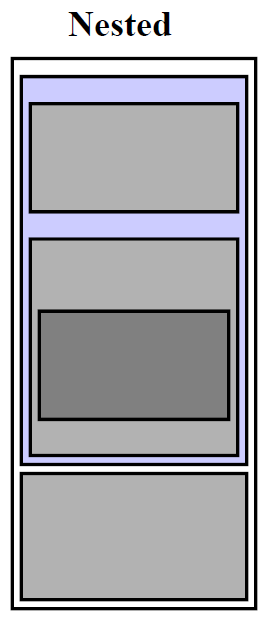
\includegraphics[scale=0.5]{rapport/5/figures/nested_block_structure}
		\end{center}	
		\caption{Illustration of the nested block structure}
		\label{nested_block_structure}
	\end{wrapfigure}


	%INCLUDE BIBLIOGRAPHY!!!	
	\begin{itemize}
	\item No identifier may be declared more than once within the same block (at the same level) %SPO
	\item For any applied occurrence there must be a corresponding occurrence, either within the same block or block which is higher up in the nesting. %SPO
	%INCLUDE BIBL...
	\end{itemize}
	
	
	Referring to figure \ref{nested_block_structure} which demonstrates the functioning of a nested block structure visually. Initially we consider how the nested block structure works in general and later an example of how the nested block structure works in the WAR programming language.
	
	One can have as many and as few blocks as needed, and every sub-block of an existing block, can use all the variables that have been declared in blocks over itself. 
	
	
	%Her kommer noget kode af vores egen for at beskrive hvordan nested block structure virker hos os.
		
\newpage
	
	
%Page 142 i Brown!! :D
		
\subsection{Type rules}
	These are the rules that checks the expressions form, and the type validity.
	
	\subsubsection*{Type rule of $<$}
		$E1 < E2$ is type correct and of type Boolean
		if $E1$ and $E2$ are type correct and of type Integer
	\subsubsection*{Type rule of $>$}
		$E1 > E2$ is type correct and of type Boolean
		if $E1$ and $E2$ are type correct and of type Integer
	\subsubsection*{Type rule of $==$}
		$E1 == E2$ is type correct and of type Boolean
		if $E1$ and $E2$ are type correct and of type Integer
	\subsubsection*{Type rule of $>=$}
		$E1 >= E2$ is type correct and of type Boolean
		if $E1$ and $E2$ are type correct and of type Integer
	\subsubsection*{Type rule of $<=$}
		$E1 <= E2$ is type correct and of type Boolean
		if $E1$ and $E2$ are type correct and of type Integer
	\subsubsection*{Type rule of $while$}
		$while(E){C}$ is type correct
		if $E$ is of type Boolean and $C$ is type correct
	\subsubsection*{Type rule of $if$}
		$if(E){C}$ is type correct
		if $E$ is of type Boolean and $C$ is type correct
	\subsubsection*{Type rule of $else if$}
		$else if(E){C}$ is type correct
		if $E$ is of type Boolean and $C$ is type correct
	\subsubsection*{Type rule of $else$}
		$else{C}$ is type correct
		if $C$ is type correct
	
	\subsubsection*{Type rule of $Position$}
		$Position(I1,I2)$ is type correct and of type Position
		if $I1$ and $I2$ are type correct and of type Integer	
	





%So U wanna BIB me? use:
% pdflatex file
% bibtex file
% pdflatex file
% pdflatex file Aight?
\bibliography{bib}
\bibliographystyle{plain}

\end{document}

%\tableofcontents

